% Options for packages loaded elsewhere
\PassOptionsToPackage{unicode}{hyperref}
\PassOptionsToPackage{hyphens}{url}
%
\documentclass[
]{book}
\usepackage{amsmath,amssymb}
\usepackage{lmodern}
\usepackage{iftex}
\ifPDFTeX
  \usepackage[T1]{fontenc}
  \usepackage[utf8]{inputenc}
  \usepackage{textcomp} % provide euro and other symbols
\else % if luatex or xetex
  \usepackage{unicode-math}
  \defaultfontfeatures{Scale=MatchLowercase}
  \defaultfontfeatures[\rmfamily]{Ligatures=TeX,Scale=1}
\fi
% Use upquote if available, for straight quotes in verbatim environments
\IfFileExists{upquote.sty}{\usepackage{upquote}}{}
\IfFileExists{microtype.sty}{% use microtype if available
  \usepackage[]{microtype}
  \UseMicrotypeSet[protrusion]{basicmath} % disable protrusion for tt fonts
}{}
\makeatletter
\@ifundefined{KOMAClassName}{% if non-KOMA class
  \IfFileExists{parskip.sty}{%
    \usepackage{parskip}
  }{% else
    \setlength{\parindent}{0pt}
    \setlength{\parskip}{6pt plus 2pt minus 1pt}}
}{% if KOMA class
  \KOMAoptions{parskip=half}}
\makeatother
\usepackage{xcolor}
\usepackage{color}
\usepackage{fancyvrb}
\newcommand{\VerbBar}{|}
\newcommand{\VERB}{\Verb[commandchars=\\\{\}]}
\DefineVerbatimEnvironment{Highlighting}{Verbatim}{commandchars=\\\{\}}
% Add ',fontsize=\small' for more characters per line
\usepackage{framed}
\definecolor{shadecolor}{RGB}{248,248,248}
\newenvironment{Shaded}{\begin{snugshade}}{\end{snugshade}}
\newcommand{\AlertTok}[1]{\textcolor[rgb]{0.94,0.16,0.16}{#1}}
\newcommand{\AnnotationTok}[1]{\textcolor[rgb]{0.56,0.35,0.01}{\textbf{\textit{#1}}}}
\newcommand{\AttributeTok}[1]{\textcolor[rgb]{0.77,0.63,0.00}{#1}}
\newcommand{\BaseNTok}[1]{\textcolor[rgb]{0.00,0.00,0.81}{#1}}
\newcommand{\BuiltInTok}[1]{#1}
\newcommand{\CharTok}[1]{\textcolor[rgb]{0.31,0.60,0.02}{#1}}
\newcommand{\CommentTok}[1]{\textcolor[rgb]{0.56,0.35,0.01}{\textit{#1}}}
\newcommand{\CommentVarTok}[1]{\textcolor[rgb]{0.56,0.35,0.01}{\textbf{\textit{#1}}}}
\newcommand{\ConstantTok}[1]{\textcolor[rgb]{0.00,0.00,0.00}{#1}}
\newcommand{\ControlFlowTok}[1]{\textcolor[rgb]{0.13,0.29,0.53}{\textbf{#1}}}
\newcommand{\DataTypeTok}[1]{\textcolor[rgb]{0.13,0.29,0.53}{#1}}
\newcommand{\DecValTok}[1]{\textcolor[rgb]{0.00,0.00,0.81}{#1}}
\newcommand{\DocumentationTok}[1]{\textcolor[rgb]{0.56,0.35,0.01}{\textbf{\textit{#1}}}}
\newcommand{\ErrorTok}[1]{\textcolor[rgb]{0.64,0.00,0.00}{\textbf{#1}}}
\newcommand{\ExtensionTok}[1]{#1}
\newcommand{\FloatTok}[1]{\textcolor[rgb]{0.00,0.00,0.81}{#1}}
\newcommand{\FunctionTok}[1]{\textcolor[rgb]{0.00,0.00,0.00}{#1}}
\newcommand{\ImportTok}[1]{#1}
\newcommand{\InformationTok}[1]{\textcolor[rgb]{0.56,0.35,0.01}{\textbf{\textit{#1}}}}
\newcommand{\KeywordTok}[1]{\textcolor[rgb]{0.13,0.29,0.53}{\textbf{#1}}}
\newcommand{\NormalTok}[1]{#1}
\newcommand{\OperatorTok}[1]{\textcolor[rgb]{0.81,0.36,0.00}{\textbf{#1}}}
\newcommand{\OtherTok}[1]{\textcolor[rgb]{0.56,0.35,0.01}{#1}}
\newcommand{\PreprocessorTok}[1]{\textcolor[rgb]{0.56,0.35,0.01}{\textit{#1}}}
\newcommand{\RegionMarkerTok}[1]{#1}
\newcommand{\SpecialCharTok}[1]{\textcolor[rgb]{0.00,0.00,0.00}{#1}}
\newcommand{\SpecialStringTok}[1]{\textcolor[rgb]{0.31,0.60,0.02}{#1}}
\newcommand{\StringTok}[1]{\textcolor[rgb]{0.31,0.60,0.02}{#1}}
\newcommand{\VariableTok}[1]{\textcolor[rgb]{0.00,0.00,0.00}{#1}}
\newcommand{\VerbatimStringTok}[1]{\textcolor[rgb]{0.31,0.60,0.02}{#1}}
\newcommand{\WarningTok}[1]{\textcolor[rgb]{0.56,0.35,0.01}{\textbf{\textit{#1}}}}
\usepackage{longtable,booktabs,array}
\usepackage{calc} % for calculating minipage widths
% Correct order of tables after \paragraph or \subparagraph
\usepackage{etoolbox}
\makeatletter
\patchcmd\longtable{\par}{\if@noskipsec\mbox{}\fi\par}{}{}
\makeatother
% Allow footnotes in longtable head/foot
\IfFileExists{footnotehyper.sty}{\usepackage{footnotehyper}}{\usepackage{footnote}}
\makesavenoteenv{longtable}
\usepackage{graphicx}
\makeatletter
\def\maxwidth{\ifdim\Gin@nat@width>\linewidth\linewidth\else\Gin@nat@width\fi}
\def\maxheight{\ifdim\Gin@nat@height>\textheight\textheight\else\Gin@nat@height\fi}
\makeatother
% Scale images if necessary, so that they will not overflow the page
% margins by default, and it is still possible to overwrite the defaults
% using explicit options in \includegraphics[width, height, ...]{}
\setkeys{Gin}{width=\maxwidth,height=\maxheight,keepaspectratio}
% Set default figure placement to htbp
\makeatletter
\def\fps@figure{htbp}
\makeatother
\setlength{\emergencystretch}{3em} % prevent overfull lines
\providecommand{\tightlist}{%
  \setlength{\itemsep}{0pt}\setlength{\parskip}{0pt}}
\setcounter{secnumdepth}{5}
\newlength{\cslhangindent}
\setlength{\cslhangindent}{1.5em}
\newlength{\csllabelwidth}
\setlength{\csllabelwidth}{3em}
\newlength{\cslentryspacingunit} % times entry-spacing
\setlength{\cslentryspacingunit}{\parskip}
\newenvironment{CSLReferences}[2] % #1 hanging-ident, #2 entry spacing
 {% don't indent paragraphs
  \setlength{\parindent}{0pt}
  % turn on hanging indent if param 1 is 1
  \ifodd #1
  \let\oldpar\par
  \def\par{\hangindent=\cslhangindent\oldpar}
  \fi
  % set entry spacing
  \setlength{\parskip}{#2\cslentryspacingunit}
 }%
 {}
\usepackage{calc}
\newcommand{\CSLBlock}[1]{#1\hfill\break}
\newcommand{\CSLLeftMargin}[1]{\parbox[t]{\csllabelwidth}{#1}}
\newcommand{\CSLRightInline}[1]{\parbox[t]{\linewidth - \csllabelwidth}{#1}\break}
\newcommand{\CSLIndent}[1]{\hspace{\cslhangindent}#1}
\ifLuaTeX
  \usepackage{selnolig}  % disable illegal ligatures
\fi
\IfFileExists{bookmark.sty}{\usepackage{bookmark}}{\usepackage{hyperref}}
\IfFileExists{xurl.sty}{\usepackage{xurl}}{} % add URL line breaks if available
\urlstyle{same} % disable monospaced font for URLs
\hypersetup{
  pdftitle={  Evaluación económica reproducible para proyectos de inversión bajo incertidumbre usando métodos cuantitativos para la toma de decisiones},
  hidelinks,
  pdfcreator={LaTeX via pandoc}}

\title{
\includegraphics[width=2in,height=\textheight]{diagramas/FQ.jpg} 
\includegraphics[width=2in,height=\textheight]{diagramas/UNAM.jpg}
Evaluación económica reproducible para proyectos de inversión bajo incertidumbre usando métodos cuantitativos para la toma de decisiones}
\author{Artur Herbert Malek Huidobro\\
415031756}
\date{2023-03-17}

\begin{document}
\maketitle

{
\setcounter{tocdepth}{1}
\tableofcontents
}
\renewcommand{\figurename}{Figura}
\renewcommand{\listfigurename}{Lista de Figuras}
\renewcommand{\listtablename}{Lista de Tablas}
\renewcommand{\tablename}{Tabla}

\listoffigures

\listoftables

\newpage

\hypertarget{introducciuxf3n}{%
\chapter{Introducción}\label{introducciuxf3n}}

El avance exponencial que hemos experimentado como sociedad, tanto en el
desarrollo de nuevas tecnologías (reflejado en el incremento del número
de patentes concedidas año con año, 391 mil patentes concedidas en 2019
comparado con 49 mil en 1963) (\protect\hyperlink{ref-Marco2015}{Marco et al. 2015}), como en el aumento del
volumen de información generada (\protect\hyperlink{ref-Holst2021}{Holst 2021}), así como en el incremento
en la rapidez con la que podemos analizarla y extraer significado de
ella (\protect\hyperlink{ref-Davenport2013}{Davenport and Diché 2013}) aunado a un ambiente de inversión de mayor
incentidumbre (\protect\hyperlink{ref-Ahir2020}{Ahir, Bloom, and Furceri 2020}) hace más crítica la evaluación de proyectos
previo a su implementación, dada la correlación existente entre el
aumento de incertidumbre y la disminución en la inversión (\protect\hyperlink{ref-Leahy1996}{Leahy and Whited 1996}).

El uso de técnicas cuantitativas para la toma de decisiones es, sin lugar
a duda, una idea que ha sido estudidada por más de seis lustros. John
Bishop, Robert Schlaifer y Howard Raiffa revolucionaron el concepto de
Toma de Decisiones por medio de la integración de conceptos de una
escuela de pensamiento estadístico en los años 50. En específico,
Raiffer y Schlaifer desarrollaron un método para cuantificar el
conocimiento subjetivo utilizando \textbf{Probabilidad Bayesiana Subjetiva}
mientras trabajaban en \textbf{Harvard Business School}
(\protect\hyperlink{ref-Mcdonald2017Golden}{McDonald 2017}), influenciando de esta manera a generaciones de
administradores educados en HBS (a través del curso de \textbf{Managerial
Economics Reporting and Control} o MERC) y por lo mismo, su efecto
debería de sentirse a través de la comunidad de negocios hasta hoy en
día. Sin embargo, resultados de un análisis de una encuesta a ejecutivos
de compañías de \textbf{Fortune 500} indican que las mayores barreras de
adopción eran (\protect\hyperlink{ref-Green1976survey}{Green, Newson, and Jones 1976}):

\begin{enumerate}
\def\labelenumi{\arabic{enumi}.}
\tightlist
\item
  Los beneficios de usar las técnicas no son claramente entendibles
  por los administradores
\item
  Los administradores no tienen el conocimiento necesario respecto a
  técnicas cuantitativas
\item
  Los administradores no fueron expuestos a técnicas cuantitativas al
  inicio de su entrenamiento.
\end{enumerate}

La lista continúa. Sin embargo, este top 3 nos ayuda a ver cierta parte
de la problemática que se relaciona al entendimiento de los métodos
cuantitativos por parte de la administración de las empresas. Esto es un
problema importante que puede ser minimizado (al menos en parte) por el
uso de tecnologías disponibles hoy en día.

Para este trabajo, se busca comparar los resultados de decisión de
inversión, para un proyecto de implementación de una nueva tecnología
en la industria química, con base en los métodos cuantitativos:
Simulación Monte Carlo, Análisis de Sensibilidad, Valor Monetario
Esperado (EMV por sus siglas en inglés) y Matriz de Toma de Decisiones
(\protect\hyperlink{ref-Stefanovic2005}{Stefanovic and Stefanovic 2005}). Esto con el fin de mostrar la diferencia entre las
decisiones que se tomarían con cada uno de los métodos por separado y
cómo se puede combinar el uso de estos métodos para mejorar la toma de
decisiones.

El utilizar R, en específico RMarkdown y paquetes del tidyverse, nos
permite crear un marco de análisis el cual es fácil de actualizar
conforme se obtenga mayor (o nueva) información de la(s) inversión(es)
que está(n) intentando analizarse. En mi experiencia en la industria,
toma mucho tiempo utilizar herramientas distintas para el análisis de la
información y para la presentación de la misma (ej. Excel y PowerPoint,
si se utilizan las herramientas de Microsoft), mientras que el modelo mismo
es más difícil de analizar, dado que la información se encuentra en cada celda
y tiene una ubicación espacial que no puede ser necesariamente intuitiva.
Incluso si se intenta utilizar esfuerzos de automatización para esto, como
macros o código en VBA, se requiere de mayor esfuerzo y es más fácil hacer
cambios sobre los documentos que causen errores al correr el código de
automatización.

El proyecto de implementación a ser evaluado es uno de ``Medicina Personalizada'';
este fue elegido con base en el impacto que puede llegar a tener,
de acuerdo al cuadrante de tendencias disruptivas y con
fines económicos de la industria química descritos en: (\protect\hyperlink{ref-Falter2017}{Falter et al. 2017}).

\newpage

\hypertarget{medicina-personalizada}{%
\section{Medicina Personalizada}\label{medicina-personalizada}}

Dado que las enfermedades son más similares a una ``red'' de actividades
aberrantes (comunicación y comportamiento celular, proteínas
multifuncionales, genes modificadores, etc.), que a una progresión
lineal de síntomas (\protect\hyperlink{ref-Li2015}{Li et al. 2015}), la medicina personalizada puede ayudar a
determinar el tratamiento apropiado para un individuo con base en
grandes cantidades de información a nivel de población (\protect\hyperlink{ref-Ho2020}{Ho et al. 2020}).

La medicina personalizada o de precisión cuenta con dos acercamientos,
el primero involucra el uso de tecnologías para adquirir y validar
información de poblaciones, tales como análisis ómico de células y
descubrimiento de biomarcadores para su subsecuente aplicación a nivel
de paciente. El segundo, involucra el uso de tecnologías para adquirir y
evaluar la información de un individuo para su propio tratamiento. El
uso de ambos acercamientos se podría realizar a través de su
integración, de manera que la información de población se utilice para
guiar qué compuesto utilizar con base en la información genética de la
persona, seguido de una dosificación dinámica guiada por información del
individuo (\protect\hyperlink{ref-Ho2020}{Ho et al. 2020}).

Para la tecnología específica a evaluar de Medicina Personalizada,
escogimos una que queda bajo el segundo acercamiento. En específico, en
una solución para dosificación dinámica, la cual se encuentra al cerca
del final de la cadena de valor, es decir, de un método de producción de
las tabletas para cada individuo.

\hypertarget{tabletas-personalizables}{%
\subsection{Tabletas Personalizables}\label{tabletas-personalizables}}

La tecnología, de Medicina Personalizada evaluada en este trabajo, está
enfocada al paso siguiente de los acercamientos descritos en la sección
anterior, en especial al segundo acercamiento con fines de dosificación
dinámica y patrón de liberación del compuesto activo en tabletas
impresas utilizando tecnología de impresión 3D.

El método propuesto por Neriah para resolver el problema de proveer
medicina personalizada a la población en general para individuos
específicos efectiva y eficientemente, es a través de la fabricación
versátil de tabletas utilizando moldes específicamente diseñados de
diferentes formas y tamaños con el fin de permitir la personalización de
los siguientes aspectos de una tableta: dósis, duración, perfil de
liberación y combinación de diferentes compuestos (\protect\hyperlink{ref-Neriah2020}{Tan et al. 2020}).

Este acercamiento para proveer medicina personalizada a la población en
general cuenta con sus desafíos logísticos, y de producción, los cuales
se podrían ver reflejados en costos operativos elevados. Continuaremos
esta discusión en la sección de resultados específica a esta tecnología.

\hypertarget{modelos-de-negocio}{%
\subsubsection{Modelos de negocio}\label{modelos-de-negocio}}

La implementación de esta tecnología se presta a dos modelos de negocio
similares, pero que divergen en el punto de producción de las tabletas
personalizadas. En el primer modelo de negocio la producción de las
tabletas personalizadas se lleva a cabo en un centro operativo que
atiende a un número definido de farmacias y hospitales que se encuentren
en la cercanía. Mientras que en el segundo modelo de negocio se producen
las tabletas en las farmacias o en los hospitales mismos.

En ambos casos el cliente final haría un chequeo inicial en el hospital
o la farmacia en donde, con la ayuda de un doctor y análisis del caso
particular del paciente, se determina la dosis, así como el perfil y
tiempo de liberación de los componentes de la tableta personalizada.
Esta información se agregaría a un expediente compartido en donde cada
orden contendría la información necesaria para producir las tabletas
según las especificaciones indicadas por el personal de salud.

La diferencia entre ambos casos de negocio radica en que uno centraliza la
producción de las tabletas y distribuye a hospitales y farmacias desde una
ubicación central, mientras que el otro busca producir las tabletas en el
lugar de entrega.

A continuación se muestran los diagramas que muestran dichos modelos de negocio.

\begin{figure}
\centering
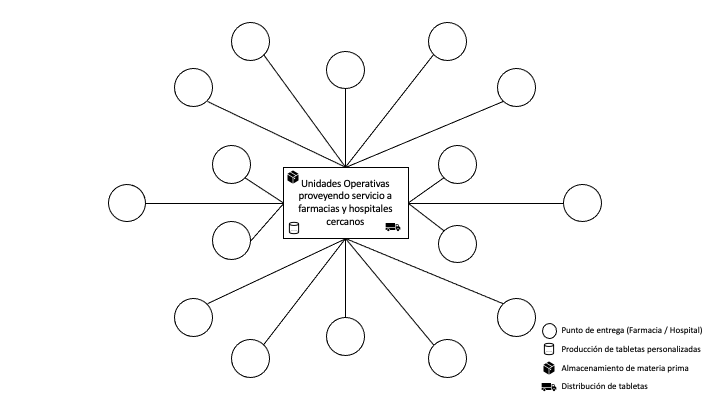
\includegraphics[width=0.9\textwidth,height=\textheight]{Diagramas/TP_Business_Model_1.png}
\caption{Diagrama de modelo de negocio con unidades operativas con producción
semi-centralizada}
\end{figure}

\begin{figure}
\centering
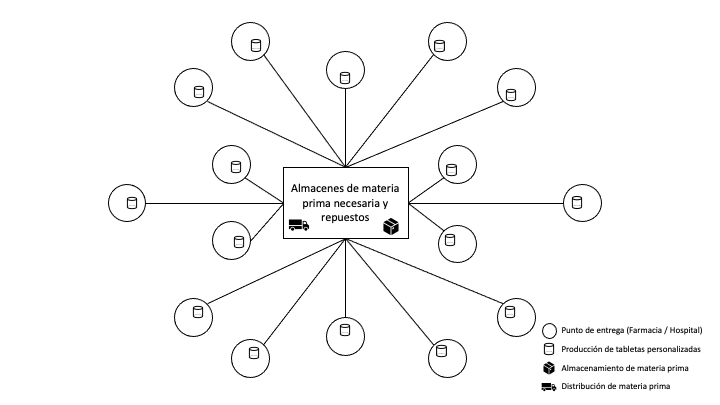
\includegraphics[width=0.9\textwidth,height=\textheight]{Diagramas/TP_Business_Model_2.png}
\caption{Diagrama de modelo de negocio con producción en cada punto de venta
(Farmacias / Hospitales)}
\end{figure}

\newpage

\hypertarget{procedimiento}{%
\chapter{Procedimiento}\label{procedimiento}}

Para el desarrollo de esta tesina se hace uso de R version 4.2.2 (2022-10-31) de forma que el trabajo aquí descrito sea totalmente reproducible. A continuación podrán observar la información de la sesión activa durante la compilación de este trabajo:

\begin{verbatim}
## R version 4.2.2 (2022-10-31)
## Platform: x86_64-apple-darwin17.0 (64-bit)
## Running under: macOS Ventura 13.2
## 
## Matrix products: default
## LAPACK: /Library/Frameworks/R.framework/Versions/4.2/Resources/lib/libRlapack.dylib
## 
## locale:
## [1] en_US.UTF-8/en_US.UTF-8/en_US.UTF-8/C/en_US.UTF-8/en_US.UTF-8
## 
## attached base packages:
## [1] stats     graphics  grDevices utils     datasets  methods   base     
## 
## other attached packages:
##  [1] webshot_0.5.4     DiagrammeR_1.0.9  data.tree_1.0.0   formattable_0.2.1 scales_1.2.1     
##  [6] knitr_1.41        EnvStats_2.7.0    forcats_0.5.2     stringr_1.5.0     dplyr_1.0.10     
## [11] purrr_0.3.5       readr_2.1.3       tidyr_1.2.1       tibble_3.1.8      ggplot2_3.4.0    
## [16] tidyverse_1.3.2   pacman_0.5.1      bookdown_0.32    
## 
## loaded via a namespace (and not attached):
##  [1] httr_1.4.4          sass_0.4.4          bit64_4.0.5         vroom_1.6.0        
##  [5] jsonlite_1.8.4      modelr_0.1.10       bslib_0.4.1         assertthat_0.2.1   
##  [9] highr_0.9           googlesheets4_1.0.1 cellranger_1.1.0    yaml_2.3.6         
## [13] pillar_1.8.1        backports_1.4.1     glue_1.6.2          digest_0.6.30      
## [17] RColorBrewer_1.1-3  rvest_1.0.3         colorspace_2.0-3    htmltools_0.5.3    
## [21] pkgconfig_2.0.3     broom_1.0.1         haven_2.5.1         processx_3.8.0     
## [25] tzdb_0.3.0          timechange_0.1.1    googledrive_2.0.0   generics_0.1.3     
## [29] farver_2.1.1        ellipsis_0.3.2      cachem_1.0.6        withr_2.5.0        
## [33] cli_3.4.1           magrittr_2.0.3      crayon_1.5.2        readxl_1.4.1       
## [37] ps_1.7.2            evaluate_0.18       fs_1.5.2            fansi_1.0.3        
## [41] xml2_1.3.3          tools_4.2.2         hms_1.1.2           gargle_1.2.1       
## [45] lifecycle_1.0.3     munsell_0.5.0       reprex_2.0.2        callr_3.7.3        
## [49] compiler_4.2.2      jquerylib_0.1.4     tinytex_0.42        rlang_1.0.6        
## [53] grid_4.2.2          rstudioapi_0.14     htmlwidgets_1.5.4   visNetwork_2.1.2   
## [57] labeling_0.4.2      rmarkdown_2.18      gtable_0.3.1        DBI_1.1.3          
## [61] R6_2.5.1            lubridate_1.9.0     bit_4.0.5           fastmap_1.1.0      
## [65] utf8_1.2.2          stringi_1.7.8       parallel_4.2.2      vctrs_0.5.1        
## [69] dbplyr_2.2.1        tidyselect_1.2.0    xfun_0.35
\end{verbatim}

\hypertarget{muxe9todos-cuantitativos-de-toma-de-decisiuxf3n}{%
\section{Métodos cuantitativos de toma de decisión}\label{muxe9todos-cuantitativos-de-toma-de-decisiuxf3n}}

En esta sección se describen los métodos cuantitativos que se usaron para el presente trabajo.

\textbf{rrr} Revisar el documento siguiente: (\protect\hyperlink{ref-Tapiero2013}{Tapiero 2013})

\textbf{rrr} Revisión de métodos de evaluación que puede ser útil para este trabajo. (\protect\hyperlink{ref-Crundwell2008}{Crundwell 2008})

\textbf{rrr} Artículo que se ve interesante para la introducción a tomar en cuenta los riesgos para la evaluación económica de proyectos de inversión (\protect\hyperlink{ref-Bartovsova2015}{Bartošová, Majerčák, and Hrašková 2015})

\hypertarget{orden-de-uso-de-los-muxe9todos}{%
\subsection{Orden de uso de los métodos}\label{orden-de-uso-de-los-muxe9todos}}

El orden de los métodos utilizado en este trabajo para la evaluación de los proyectos de inversión es el representado en el siguiente diagrama:

\begin{figure}
\centering
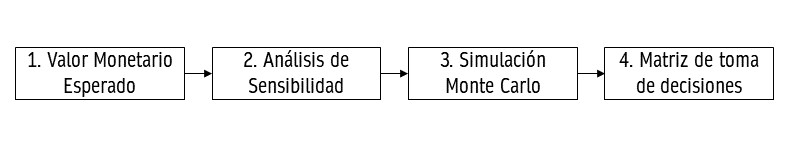
\includegraphics[width=0.9\textwidth,height=\textheight]{Diagramas/OrdenMetodos.jpg}
\caption{Diagrama del orden de uso de los métodos cuantitativos}
\end{figure}

La razón de esto es la siguiente:

\begin{enumerate}
\def\labelenumi{\arabic{enumi}.}
\tightlist
\item
  El método de valor monetario esperado lo utilizamos como primer acercamiento a la evaluación de los proyectos ya que con éste podemos evaluar el proyecto utilizando escenarios simples con base en una probabilidad asociada a cada escenario.
\item
  El método de análisis de sensibilidad nos permite cuantificar el impacto sobre la evaluación del proyecto que produce el cambio sobre las diferentes variables del modelo. Esto nos permite identificar las variables que tienen el mayor impacto sobre la evaluación del proyecto.
\item
  El método Monte Carlo utiliza distribuciones de probabilidad (en específico para las variables que tienen un mayor impacto sobre el proyecto), con el fin de calcular la confianza que se tiene sobre el resultado de la evaluación.
\item
  El método de matriz de toma de decisiones requiere de la cuantificación de diferentes factores de decisión entre los cuales se incluye el retorno esperado que calculamos con el método de simulación Monte Carlo. Esto nos sirve para tomar decisiones, entre diferentes alternativas de inversión, cuando se tiene más de un sólo parámetro de decisión.
\end{enumerate}

\hypertarget{ecuaciones-utilizadas}{%
\subsection{Ecuaciones utilizadas}\label{ecuaciones-utilizadas}}

\textbf{Flujo de Caja Libre (FCF)}
La ecuación (\eqref{eq:fcfeq}) para el cálculo del flujo de caja libre \emph{``Free Cash Flow''} utilizada a lo largo del trabajo fue tomada de (\protect\hyperlink{ref-Berk2017}{Berk and DeMarzo 2017}).

\begin{equation}
  FCF = (Ing. - Cost. - Depr.) * (1-\tau_{c}) + Depr. - Inv. - \Delta CTN
  \label{eq:fcfeq}
\end{equation}

Donde:

\begin{itemize}
\tightlist
\item
  \emph{FCF} significa Flujo de Caja Libre (o Free Cash Flow)
\item
  \emph{Ing.} representa los ingresos
\item
  \emph{Cost.} representa los costos
\item
  \emph{Depr.} representa la depreciación
\item
  \(\tau_{c}\) representa la tasa gravable de impuestos
\item
  \emph{Inv.} representa la inversión
\item
  \(\Delta CTN\) representa el cambio en el capital de trabajo neto
\end{itemize}

\textbf{Valor Presente Neto (NPV)}
La ecuación (\eqref{eq:npveq}) utilizada para el Valor Presente Neto es una
adaptación de la ecuación para el método \emph{``The Present Worth Method''} tomada de (\protect\hyperlink{ref-Sullivan2015}{Sullivan, Wicks, and Koelling 2015}).

\begin{equation}
  NPV = \sum_{k=0}^{N}FCF_{k} (1+i)^{-k}
  \label{eq:npveq}
\end{equation}

Donde:

\begin{itemize}
\tightlist
\item
  \emph{i} representa la tasa de interés efectiva (effective interest rate) por cada periodo
\item
  \emph{k} representa el índice de cada periodo (\(0 \le k \le N\))
\item
  \(FCF_{k}\) representa el flujo de caja libre al final del periodo \emph{k}
\item
  \emph{N} representa el número de periodos en el horizonte de la evaluación.
\end{itemize}

\hypertarget{valor-monetario-esperado}{%
\subsection{Valor Monetario Esperado}\label{valor-monetario-esperado}}

Para los fines de este trabajo realizamos el cálculo del valor monetario esperado dado por la función \eqref{eq:emveq}:

\begin{equation}
  EMV = \sum_{i=0}^{n}NPV_{i} \cdot p_{i}
  \label{eq:emveq}
\end{equation}

Donde:

\begin{itemize}
\tightlist
\item
  \emph{EMV} representa el valor monetario esperado (o Expected Monetary Value)
\item
  \emph{i} representa el índice de los posibles escenarios
\item
  \emph{n} representa el número de posibles escenarios
\item
  \(NPV_{i}\) representa el valor presente neto de los posibles escenarios
\item
  \(p_{i}\) representa la probabilidad de que dicho valor presente neto \emph{i} se materialice
\end{itemize}

Para fines de comparación utilizamos la metodología de análisis de problemas de toma de decisiones complejas basada en \emph{Cumulative Prospect Theory} propuesta en (\protect\hyperlink{ref-Dudzinska2018}{Dudzińska-Baryła 2018}).

\textbf{Diagrama de solución}

\begin{figure}
\centering
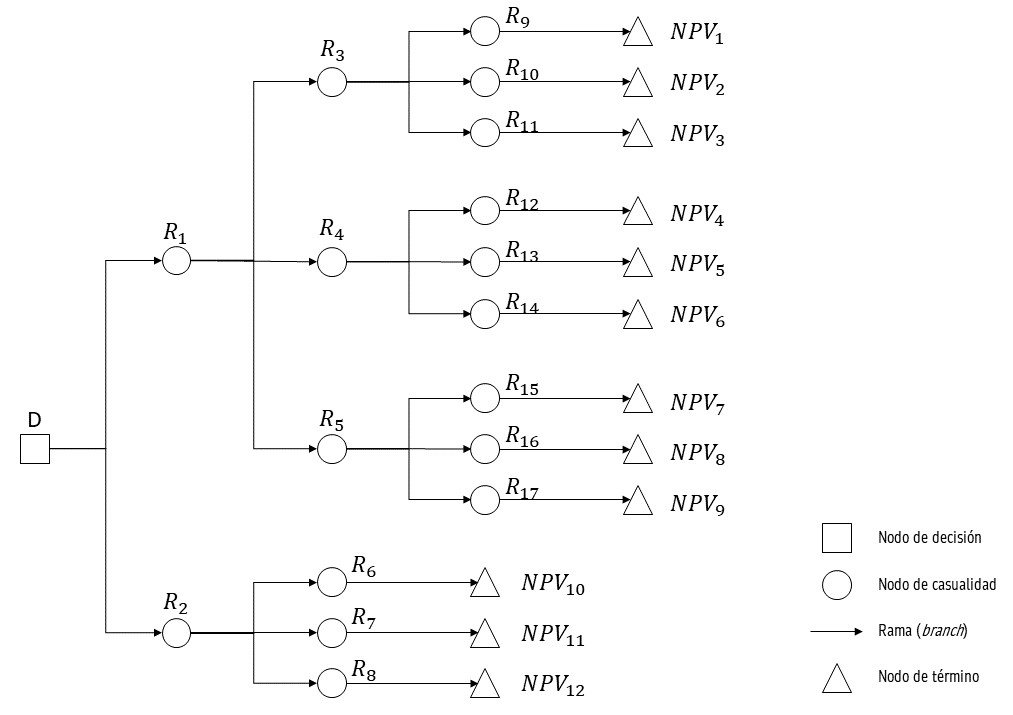
\includegraphics[width=0.9\textwidth,height=\textheight]{Diagramas/DecisionTree.jpg}
\caption{Diagrama de arbol de decisión tomando con tres escenarios por cada nodo de casualidad}
\end{figure}

El cálculo del \emph{EMV} se realizará a través de árboles de decisión (\emph{decision trees}) en donde se representen tres posibles escenarios relacionados a la decisión de llevar a cabo la inversión:

\begin{itemize}
\tightlist
\item
  \emph{Escenario bajo}: representa la posibilidad de que el valor sea menor al escenario medio (ej. 15\%)
\item
  \emph{Escenario medio}: representa el valor más probable resultado de la investigación (ej. 70\%)
\item
  \emph{Escenario alto}: representa la posibilidad de que el valor sea mayor al resultado de la investigación (ej. 15\%)
\end{itemize}

Esto se llevó a cabo para cada uno de los tres componentes más importantes del modelo: ingresos, costos e inversión.

\textbf{rrr} La siguiente referencia tiene información del algoritmo (\protect\hyperlink{ref-Prellezo2017}{Prellezo 2017})

\hypertarget{anuxe1lisis-de-sensibilidad}{%
\subsection{Análisis de Sensibilidad}\label{anuxe1lisis-de-sensibilidad}}

El análisis de sensibilidad es un grupo de métodos que nos ayuda a validar el modelo, a calibrarlo y a enfocar los esfuerzos de recolección de información sobre las variables que tienen un mayor impacto sobre el modelo en cuestión (\protect\hyperlink{ref-Borgonovo2017}{Borgonovo et al. 2017}). Ya que si las decisiones son insensibles ante cambios sobre un aspecto del modelo, entonces no hay necesidad de modelar a mayor detalle ese aspecto en particular (\protect\hyperlink{ref-Felli2004}{Felli and Hazen 2004}).

Estos métodos se pueden dividir en dos grupos distintivos: métodos dedicados al modelo en cuestión y métodos agnósticos al modelo. Los primeros buscan responder preguntas específicas al modelo, mientras que los segundos buscan responder preguntas más generales (\protect\hyperlink{ref-Borgonovo2017}{Borgonovo et al. 2017}).

Borgonovo explica la importancia de la adecuada formulación de la pregunta de análisis de sensibilidad y presenta las siguientes configuraciones que han encontrado a lo largo de su investigación:

\begin{enumerate}
\def\labelenumi{\arabic{enumi}.}
\tightlist
\item
  Priorización de parámetros del modelo
\item
  Fijación de parámetros del modelo
\item
  Estructura del modelo
\item
  Dirección del cambio
\item
  Estabilidad
\end{enumerate}

Este trabajo utiliza principalmente las primeras dos configuraciones con el fin de definir qué parámetros deben de ser estudiados a mayor detalle para la simulación Monte Carlo.

El método principal que revisamos en este trabajo es el método determinístico de diagramas tornado.

\newpage

\textbf{Diagrama de solución}\\
El siguiente diagrama muestra el esquema de solución para el análisis de sensibilidad utilizando el método determinístico de diagrama de tornado.

\begin{figure}
\centering
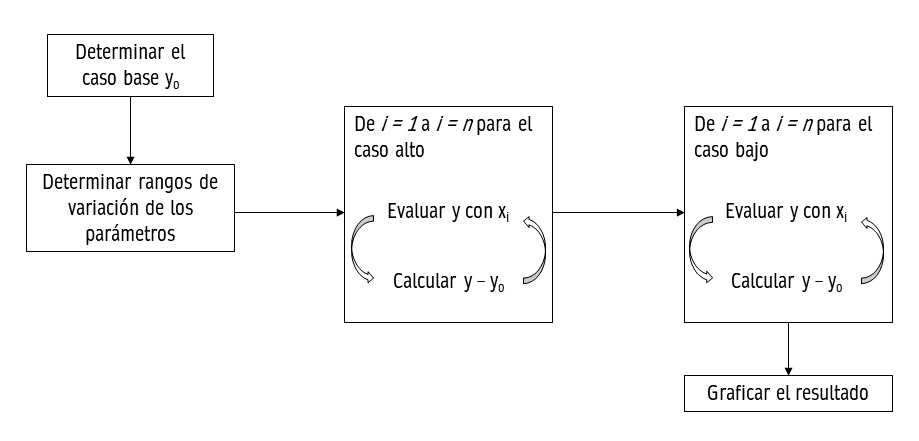
\includegraphics[width=0.9\textwidth,height=\textheight]{Diagramas/AnalisisSensibilidad.jpg}
\caption{Diagrama de Solución de Análisis de Sensibilidad}
\end{figure}

\begin{figure}

{\centering 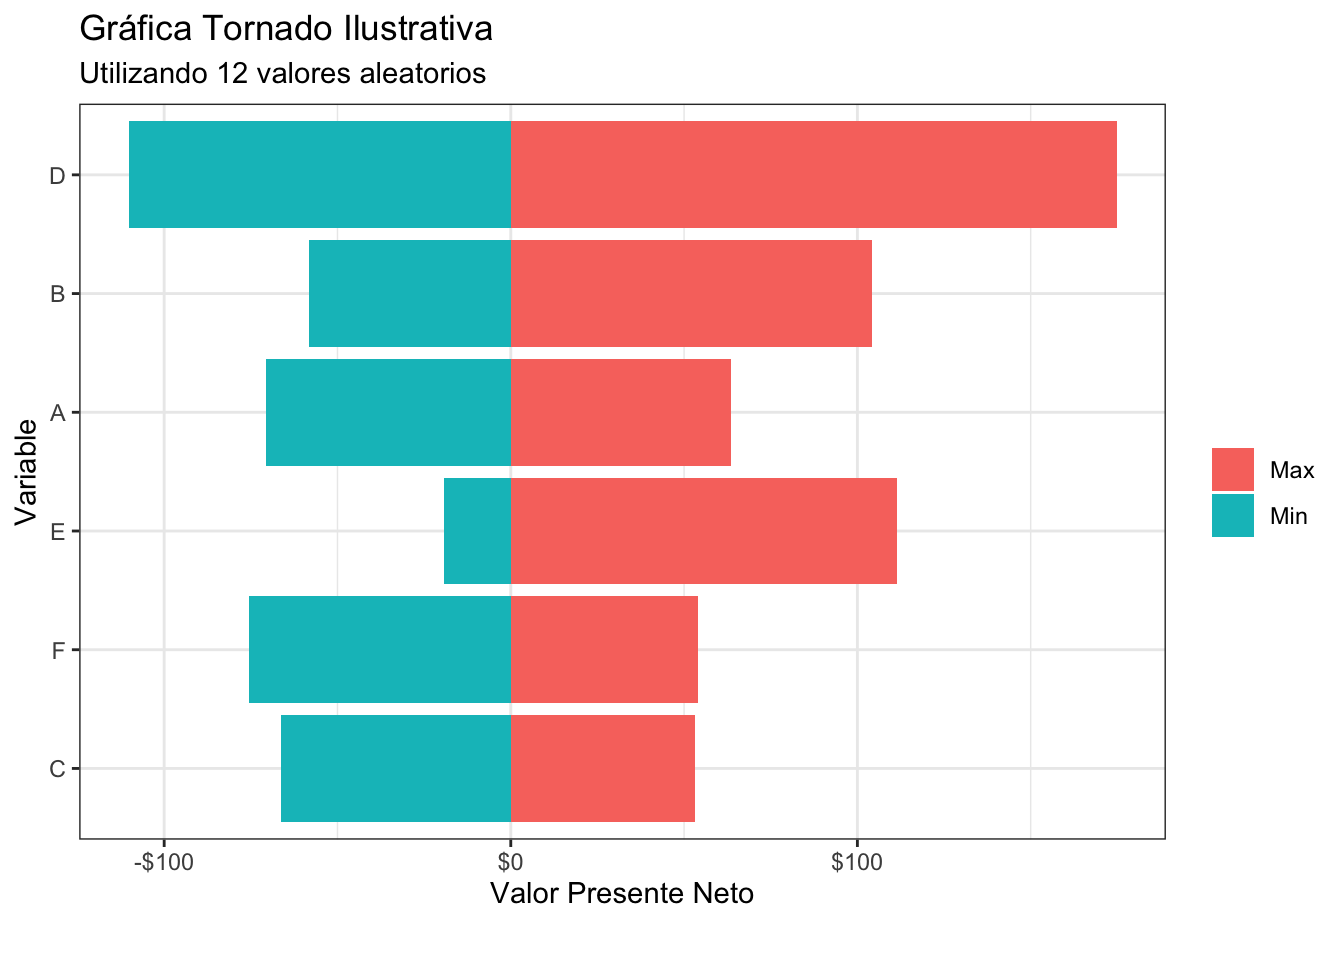
\includegraphics[width=0.65\linewidth]{_main_files/figure-latex/tornadotest-1} 

}

\caption{Ejemplo de una gráfica tornado con 6 variables y 6 pares de números aleatorios representando valores máximos y mínimos}\label{fig:tornadotest}
\end{figure}

\textbf{rrr} Un ejemplo de evaluación económica con análisis de sensibilidad para revisar (\protect\hyperlink{ref-Lee2017}{Lee, Chae, et al. 2017})

\newpage

\hypertarget{simulaciuxf3n-monte-carlo}{%
\subsection{Simulación Monte Carlo}\label{simulaciuxf3n-monte-carlo}}

El método Monte Carlo es una técnica para analizar fenómenos por medio de algoritmos computacionales basados, en esencia, en la generación de números aleatorios. De hecho, uno de los primeros usos de la computadora fue la solución de problemas a través del uso de Métodos Monte Carlo. Hoy en día los métodos de simulación Monte Carlo siguen teniendo un domino casi exclusivo sobre la simulación de interacciones complejas en cualquier área donde los modelos cuantitativos son posibles (\protect\hyperlink{ref-Shonkwiler2009}{Shonkwiler and Mendivil 2009}).

rrr Temas más avanzados con aplicación en finanzas (\protect\hyperlink{ref-Shonkwiler2013}{Shonkwiler 2013})

rrr Framework ejemplo (\protect\hyperlink{ref-Dheskali2020}{Dheskali, Koutinas, and Kookos 2020})

rrr Ejemplo de simulación Monte Carlo para la inversión en tecnología de tercera generación de plantas nucleares (\protect\hyperlink{ref-Wealer2021}{Wealer et al. 2021})

rrr Ejemplo de simulación Monte Carlo para la evaluación económica de producción de hidrógeno (\protect\hyperlink{ref-Lee2017economic}{Lee, Heo, et al. 2017})

\textbf{Números aleatorios}

Para el método de simulación Monte Carlo se necesita generar valores aleatorios (una secuencia de estos) para las variables con mayor impacto sobre el resultado de la evaluación del proyecto.

Una secuencia de números aleatorios se define como una secuencia R1, R2,\ldots{} donde Ri\textasciitilde U(0,1) para todo i donde Ri sea independiente de Rj para todos los casos donde i != j. (\protect\hyperlink{ref-Dagpunar2007}{Dagpunar 2007})

El lenguaje R ya contiene funciones que nos permiten obtener secuencias de números aleatorios: \emph{rnorm} para secuencias aleatorias de números con distribución normal, \emph{rweibull} de distribución Weibull, \emph{rcauchy} para distribución Cauchy, etc.

\newpage

\textbf{Diagrama de solución}

El siguiente diagrama muestra el flujo de información a través de las funciones utilizadas para la evaluación por el método de Simulación Monte Carlo:

\begin{figure}
\centering
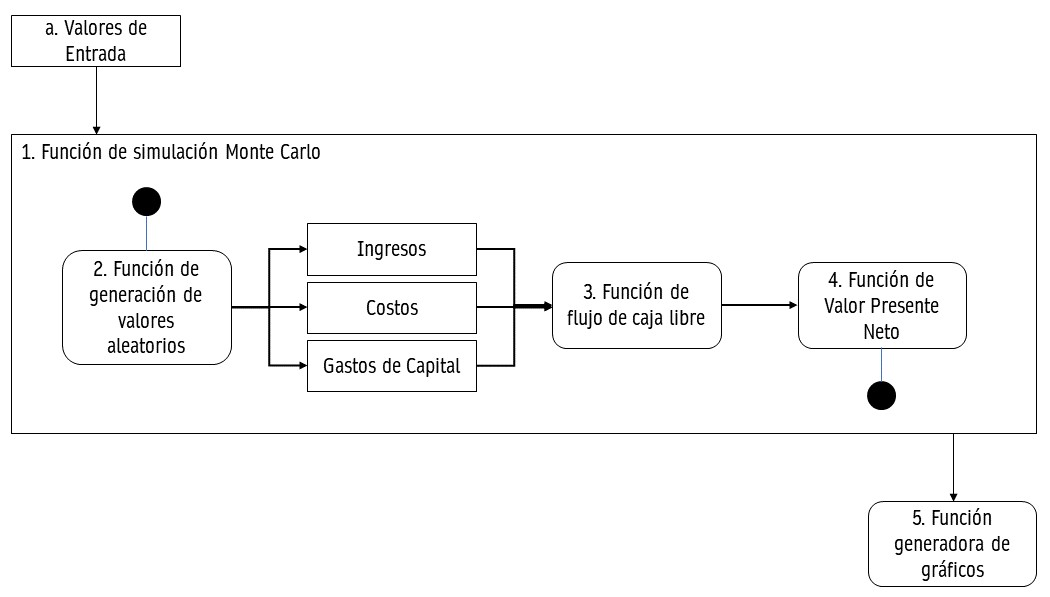
\includegraphics[width=0.9\textwidth,height=\textheight]{Diagramas/DiagramaMonteCarlo.jpg}
\caption{Diagrama de Solución Monte Carlo}
\end{figure}

Para utilizar el método de simulación Monte Carlo se desarrollaron 5 funciones (1. a 5. del diagrama) las cuales cumplen las siguientes funciones:

\begin{enumerate}
\def\labelenumi{\arabic{enumi}.}
\tightlist
\item
  Función que recibe los valores de entrada para evaluar el proyecto específico (número de periodos a evaluar, número de simulaciones a realizar, etc.) y llama a las demás funciones el número de veces especificado.
\item
  Función que genera los valores aleatorios para calcular los ingresos, costos y/o gastos de capital. Esta función como valor de entrada necesita que se especifique el tipo de distribución de probabilidad a utilizar, el caso estándar utiliza la distribución normal para calcular los valores.
\item
  Función que calcula el flujo de caja libre de efectivo tomando como valor de entrada las variables descritas en la sección de ecuaciones utilizadas.
\item
  Función que calcula el valor presente neto del flujo de caja libre calculado previamente.
\item
  Función que toma la información generada y genera las gráficas para su visualización.
\end{enumerate}

\newpage

\hypertarget{matriz-de-toma-de-decisiones}{%
\subsection{Matriz de Toma de Decisiones}\label{matriz-de-toma-de-decisiones}}

Las metodologías, conceptos, modelos y técnicas utilizadas como soporte para la toma de decisiones, tienen como objetivo incrementar la consistencia entre el proceso de toma de decisiones con las metas y con el sistema de valores establecidos por el individuo o el grupo de individuos que buscan llegar a una decisión, es por esto que un problema de decisión no puede considerarse como un objeto independiente y completamente objetivo, sino que debe de considerarse en su relación con el individuo (o individuos) y la realidad (\protect\hyperlink{ref-Azzabi2020}{Azzabi et al. 2020}).

Los métodos de decisión utilizando múltiples criterios se pueden dividir en los siguientes (\protect\hyperlink{ref-Azzabi2020}{Azzabi et al. 2020}):

\begin{itemize}
\tightlist
\item
  Compensatorio: Compensación absoluta entre las diferentes evaluaciones (ej. Método de suma ponderada).
\item
  Compensación parcial: Compensación parcial entre las diferentes evaluaciones.
\item
  Sin compensación: No hay compensación entre las diferentes evaluaciones o dimensiones de la decisión.
\end{itemize}

El acercamiento de toma de decisión multi-criterio (MCDA o Multi-Criteria Decision Approach) es tanto un marco teórico como un conjunto de técnicas, para la ayuda en la toma de decisiones, que tienen la finalidad de proveer con un orden de preferencia de opciones, de mayor a menor preferencia, con base en una serie de objetivos definidos (a lo que estaremos llamando sistema de valores en este trabajo) que pueden tener una naturaleza tanto monetaria como no monetaria (\protect\hyperlink{ref-Azzabi2020}{Azzabi et al. 2020}). Esto nos permite simplificar un problema de decisión complejo en una serie de componentes sobre los cuales podemos utilizar nuestro sistema de valores al momento de llevar a cabo el proceso de decisión.

Pasos para realizar el MCDA (\protect\hyperlink{ref-Azzabi2020}{Azzabi et al. 2020}):

\begin{enumerate}
\def\labelenumi{\arabic{enumi}.}
\tightlist
\item
  Establecer el contexto de decisión (o sistema de valores)
\item
  Identificar las opciones
\item
  Identificar criterios y subcriterios
\item
  Puntuación y compensación
\item
  Evaluar los criterios para cada opción
\end{enumerate}

\textbf{Sistema de valores}

A continuación se definen los elementos del sistema de valores utilizado en este trabajo para la toma de decisión de inversión.

\textbf{Criterios y subcriterios}

Los \emph{criterios} pueden definirse como la base para la evaluación de diferentes alternativas, ya que son una medida del rendimiento utilizado para evaluar las alternativas de decisión. Ya sean estos cuantitativos o cualitativos, aunque normalmente estos últimos se traducen a una escala numérica (\protect\hyperlink{ref-Korhonen2020}{Korhonen, Wallenius, et al. 2020}).

Los criterios a utilizar en este análisis son:

\begin{enumerate}
\def\labelenumi{\arabic{enumi}.}
\tightlist
\item
  Maximizar Valor Presente Neto
\item
  Maximizar beneficio social
\item
  Minimizar impacto ambiental
\end{enumerate}

\textbf{Puntuación y compensación}

Para este trabajo el valor relativo de los criterios se basa en el Proceso Analítico Jerárquico (\emph{AHP o Analytic Hierarchy Process}). Este es un acercamiento sistemático para el análisis de decisiones complejas originalmente desarrollado por \emph{Thomas L. Saaty} en los años setenta. Este acercamiento tiene el objetivo de encontrar una solución que mejor se adecue a las metas de los tomadores de decisión, al mismo tiempo que les ayuda a comprender de mejor forma lo que en realidad quieren (\protect\hyperlink{ref-Korhonen2020}{Korhonen, Wallenius, et al. 2020}).

Un ejemplo de valores relativos se pueden observar en la tabla \ref{tab:critcomparison}.

\begin{table}

\caption{\label{tab:critcomparison}Comparativo del valor de los criterios (AHP)}
\centering
\begin{tabular}[t]{l|c|c|c}
\hline
Criterio & VPN & Beneficio Social & Impacto Ambiental\\
\hline
VPN & 1 & 1/2 & 1/4\\
\hline
Beneficio Social & 2 & 1 & 1/2\\
\hline
Impacto Ambiental & 4 & 2 & 1\\
\hline
\end{tabular}
\end{table}

Esta tabla muestra la importancia relativa entre los criterios, siendo las columnas la representación de la importancia relativa del criterio mostrado en el renglón en relación al criterio que encabeza la columna. Si revisamos la tabla \ref{tab:critcomparison} podemos observar que el valor Presente Neto tiene una importancia relativa de 1 contra si mismo, mientras que el criterio de Beneficio Social tiene una importancia relativa 2 veces mayor que el VPN y el Impacto Ambiental tiene una importancia relativa 4 veces mayor al VPN. Si continuamos a la siguiente columna podemos ver que el VPN tiene una importancia 2 veces menor al Beneficio Social y así sucesivamente.

(\protect\hyperlink{ref-CISL2019}{Cambridge Institute for Sustainability Leadership (CISL) 2019})

\newpage

\hypertarget{prueba-del-funcionamiento-de-los-muxe9todos-cuantitativos}{%
\section{Prueba del funcionamiento de los métodos cuantitativos}\label{prueba-del-funcionamiento-de-los-muxe9todos-cuantitativos}}

Cuando se genera cualquier modelo es importante hacer pruebas de
funcionamiento básico antes de utilizar los valores reales. Esto permite
corregir cualquier error que pueda no ser aparente a primera vista una
vez que se intenta utilizar con valores reales, así como para visualizar
posibles problemas que puedan presentarse a futuro.

Como primer prueba, revisaremos el funcionamiento de la fórmula de valor
presente neto utilizando los flujos de efectivo mostrados en la tabla
\ref{tab:testcashflow1}:

\begin{table}

\caption{\label{tab:testcashflow1}Flujos de efectivo de prueba}
\centering
\begin{tabular}[t]{l|c}
\hline
periods & cashflow\\
\hline
0 & \$-5,000\\
\hline
1 & \$1,000\\
\hline
2 & \$1,000\\
\hline
3 & \$1,000\\
\hline
4 & \$1,000\\
\hline
5 & \$1,000\\
\hline
6 & \$1,000\\
\hline
7 & \$1,000\\
\hline
8 & \$1,000\\
\hline
9 & \$1,000\\
\hline
10 & \$1,000\\
\hline
\end{tabular}
\end{table}

Si utilizamos una tasa de descuento de 8.00\% obtenemos un
valor presente neto de \$1,710.08. Lo cual debería de concordar con un
valor calculado manualmente de \$1,710.08 usando los principios de flujo
de efectivo descontado revisados en la parte de metodología.

\newpage

\hypertarget{valor-monetario-esperado-1}{%
\subsection{Valor Monetario Esperado}\label{valor-monetario-esperado-1}}

\textbf{Datos ilustrativos} \newline Para realizar nuestra prueba de cálculo
de EMV, podemos utilizar el siguiente ejemplo:

Una decisión de inversión en una nueva tecnología que permitiría
disminuir el costo de electricidad de una planta de producción de
estireno (mediante la reducción de la demanda energética comparado con
la tecnología antigua). Supongamos para este ejemplo que los nodos de
casualidad relevantes son los siguientes:

\begin{itemize}
\tightlist
\item
  Costo de la implementar la tecnología
\item
  Costo de la electricidad
\end{itemize}

Estamos suponiendo dentro del costo de implementación el costo de
oportunidad de cerrar la planta de producción. El costo alto o bajo en
gran parte se estaría viendo afectado por el tiempo que debe de quedar
cerrada la planta para la instalación y pruebas relacionadas.

Para ambos costos revisaremos solo dos casos, uno bajo y otro alto. Los
valores específicos que usaremos se pueden encontrar en la tabla
\ref{tab:testemv1}.

\begin{table}

\caption{\label{tab:testemv1}Valores para prueba de funcionamiento de EMV}
\centering
\begin{tabular}[t]{l|c|c}
\hline
Variable & Alto & Bajo\\
\hline
Costo Implementación & \$20,000 & \$10,000\\
\hline
Costo Electricidad & \$100 & \$50\\
\hline
\end{tabular}
\end{table}

Al igual, imaginemos que por especificaciones de la tecnología sabemos
que vamos a necesitar de 500 watts anuales bajo la tecnología
nueva, a comparación de 800 watts anuales requeridos con la
tecnología antigua.

La estructura del arbol de decisión para este ejemplo se puede
visualizar en la figura \ref{fig:testemv2}:

\begin{figure}

{\centering \includegraphics[width=0.9\linewidth]{_main_files/figure-latex/testemv2-1} 

}

\caption{Árbol de Decisión para el ejemplo de inversión}\label{fig:testemv2}
\end{figure}

Utilizando los valores previamente especificados podemos calcular los
valores para cada una de las ramas, así como los valores monetarios
esperados para cada uno de los nodos de decisión, cuyos resultados los
podemos observar en la tabla \ref{tab:testemv3}.

\begin{table}

\caption{\label{tab:testemv3}Resultados de prueba de Valor Monetario Esperado}
\centering
\begin{tabular}[t]{l|c|c}
\hline
Nivel & Probabilidad & NVP\\
\hline
Invertir? & NA & \$-826,376\\
\hline
¦--Si & NA & \$-327,068\\
\hline
¦   ¦--Costo Bajo de Implementacion & 50.00\% & \$-322,068\\
\hline
¦   ¦   ¦--Costo Alto de Electricidad & 60.00\% & \$-400,085\\
\hline
¦   ¦   °--Costo Bajo de Electricidad & 40.00\% & \$-205,042\\
\hline
¦   °--Costo Alto de Implementacion & 50.00\% & \$-332,068\\
\hline
¦       ¦--1 Costo Alto de Electricidad & 60.00\% & \$-410,085\\
\hline
¦       °--1 Costo Bajo de Electricidad & 40.00\% & \$-215,042\\
\hline
°--No & NA & \$-499,308\\
\hline
¦--2 Costo Alto de Electricidad & 60.00\% & \$-624,135\\
\hline
°--2 Costo Bajo de Electricidad & 40.00\% & \$-312,068\\
\hline
\end{tabular}
\end{table}

Otra forma de visualizar nuestros resultados, que puede llegar ser más
amigable, se encuentra en la figura \ref{fig:testemv4}:

\begin{figure}

{\centering \includegraphics[width=0.9\linewidth]{_main_files/figure-latex/testemv4-1} 

}

\caption{Árbol de Decisión para el ejemplo de inversión con valores calculados de EMV}\label{fig:testemv4}
\end{figure}

En este ejemplo podemos observar que la opción con el mayor EMV es
aquella en donde se toma la decisión de instalar la nueva tecnología con
el fin de disminuir el requerimiento energético de la planta.

Como podemos observar, los valores de EMV de los nodos de casualidad son
iguales a la suma producto de los valores de NPV de los nodos \emph{hijos} y
la probabilidad de que ocurra el caso.

Con este ejemplo se demuestra el correcto funcionamiento de las
funciones de solución para el método de Valor Monetario Esperado.

\newpage

\hypertarget{anuxe1lisis-de-sensibilidad-1}{%
\subsection{Análisis de Sensibilidad}\label{anuxe1lisis-de-sensibilidad-1}}

Para comprobar el funcionamiento de la solución de análisis de
sensibilidad podemos usar el siguiente ejemplo adaptado de
(\protect\hyperlink{ref-Sullivan2015}{Sullivan, Wicks, and Koelling 2015}), ejemplo 11-15.

En ese ejemplo se analiza la inversión en un sistema de visión utilizado
por el servicio postal para ordenar correos.

Este problema tiene 4 variables sujetas a variación:

\begin{itemize}
\tightlist
\item
  Inversión de Capital
\item
  Gasto Anual
\item
  Ahorro Anual
\item
  TMAR (Tasa Mínima Aceptable de Retorno)
\end{itemize}

Además de esto, necesitamos una variable que defina el periodo de
evaluación de la inversión. Para fines de este ejemplo, este periodo
será estático a través de todos los casos.

Podemos observar los valores base en la tabla \ref{tab:testsens1}:

\begin{table}

\caption{\label{tab:testsens1}Valores de caso base para prueba de Análisis de Sensibilidad}
\centering
\begin{tabular}[t]{l|c}
\hline
variable & valor\\
\hline
Inversion.Capital & 1,100,000.00\\
\hline
Gasto.Anual & 200,000.00\\
\hline
Ahorro.Anual & 500,000.00\\
\hline
TMAR & 0.10\\
\hline
Periodo & 5.00\\
\hline
\end{tabular}
\end{table}

Utilizando estos valores para replicar sobre el periodo de análisis de
la inversión obtenemos los flujos de efectivo mostrados en la tabla
\ref{tab:testsens2}:

\begin{table}

\caption{\label{tab:testsens2}Flujos de efectivo de caso base para prueba de Análisis de Sensibilidad}
\centering
\begin{tabular}[t]{l|c}
\hline
periodo & cashflow\\
\hline
0 & \$-800,000\\
\hline
1 & \$300,000\\
\hline
2 & \$300,000\\
\hline
3 & \$300,000\\
\hline
4 & \$300,000\\
\hline
\end{tabular}
\end{table}

Utilizando los valores de la tabla \ref{tab:testsens2} calculamos el
valor presente neto en \$150,959.63. Lo cual muestra que el caso base
es rentable.

Ahora proseguiremos a revisar la sensibilidad a los cambios sobre las
cuatro variables que mencionamos previamente. Para esto vamos a
especificar un +20\% en el caso alto y un -20\% en un caso bajo. Como ya
habíamos comentado, el periodo se mantendrá constante.

\begin{table}

\caption{\label{tab:testsens3}Especificación de variación para prueba de Análisis de Sensibilidad}
\centering
\begin{tabular}[t]{l|c|c}
\hline
variable & bajo & alto\\
\hline
Inversion.Capital & -20.00\% & 20.00\%\\
\hline
Gasto.Anual & -20.00\% & 20.00\%\\
\hline
Ahorro.Anual & -20.00\% & 20.00\%\\
\hline
TMAR & -20.00\% & 20.00\%\\
\hline
Periodo & 0.00\% & 0.00\%\\
\hline
\end{tabular}
\end{table}

Estos valores de especificación de los casos alto y bajo para cada una
de las variables nos permite calcular el valor presente neto modificando
cada una de las variables a su caso particular, mientras que los demás
valores se mantienen como los valores del caso base. Estos valores de
NPV los podemos ver en la tabla \ref{tab:testsens4}.

\begin{table}

\caption{\label{tab:testsens4}Valores de NPV para prueba de Análisis de Sensibilidad}
\centering
\begin{tabular}[t]{l|c|c|c}
\hline
variable & caso & npv & diff\\
\hline
Inversion.Capital & alto & \$-69,040 & \$-220,000\\
\hline
Gasto.Anual & alto & \$-15,835 & \$-166,795\\
\hline
Ahorro.Anual & alto & \$567,946 & \$416,987\\
\hline
TMAR & alto & \$111,205 & \$-39,755\\
\hline
Inversion.Capital & bajo & \$370,960 & \$220,000\\
\hline
Gasto.Anual & bajo & \$317,754 & \$166,795\\
\hline
Ahorro.Anual & bajo & \$-266,027 & \$-416,987\\
\hline
TMAR & bajo & \$193,638 & \$42,678\\
\hline
\end{tabular}
\end{table}

Lo cual nos permite realizar nuestra gráfica de tornado, la cual podemos
observar en la figura \ref{fig:testsens5}.

\begin{figure}

{\centering 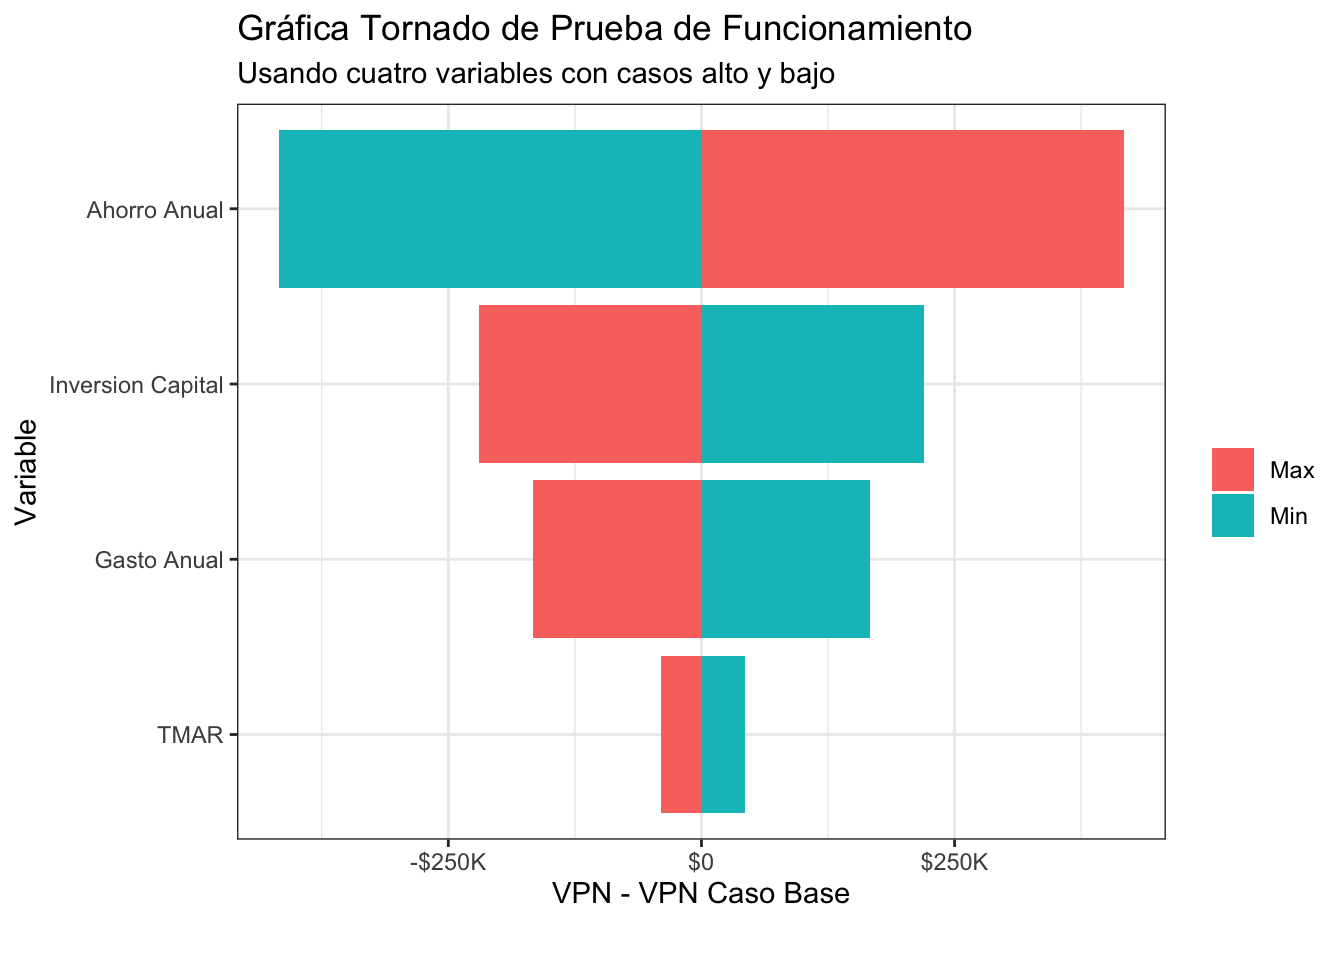
\includegraphics[width=0.65\linewidth]{_main_files/figure-latex/testsens5-1} 

}

\caption{Gráfica de Tornado de valores de prueba de funcionamiento}\label{fig:testsens5}
\end{figure}

Como podemos observar en la gráfica tornado (figura
\ref{fig:testsens5}), el mayor impacto proviene de la variable de
Ahorro Anual, seguida de la Inversión de Capital. Lo cual nos indicaría
que son las variables que deben de ser detalladas a mayor nivel en
análisis subsecuentes por el impacto que tendría en la decisión de
inversión.

Podemos observar en la gráfica que el -Valor Presente Neto- tiene una
correlación positiva con el Ahorro Anual, mientras que tiene una
correlación negativa con la Inversión de Capital, el Gasto Anual y la
TMAR, como era esperado.

\newpage

\hypertarget{simulaciuxf3n-monte-carlo-1}{%
\subsection{Simulación Monte Carlo}\label{simulaciuxf3n-monte-carlo-1}}

Para el ejemplo de simulación Monte Carlo vamos a seguir el siguiente
flujo:

\begin{itemize}
\tightlist
\item
  Definir los valores medios
\item
  Realizar el cálculo para una simulación
\item
  Mostrar que se obtiene el mismo valor con la función Monte Carlo
\item
  Mostrar los resultados de 1000 simulaciones
\end{itemize}

\begin{table}

\caption{\label{tab:tabMonteTest1}Valores caso base de Prueba Monte Carlo}
\centering
\begin{tabular}[t]{l|c|c|c|l|c|c}
\hline
tipo & periodo & material & volumen & precio & dist vol & dist pre\\
\hline
Producto & 1 & Producto1 & 1000 & \$5.00 & normal & normal\\
\hline
Producto & 1 & Producto2 & 500 & \$3.00 & normal & normal\\
\hline
Material & 1 & Material1 & 500 & \$1.00 & cauchy & normal\\
\hline
Material & 1 & Material2 & 800 & \$1.50 & cauchy & normal\\
\hline
Material & 1 & Material3 & 200 & \$2.00 & cauchy & normal\\
\hline
Utility & 1 & Electricidad & 100 & \$0.05 & poisson & cauchy\\
\hline
Utility & 1 & Gas & 50 & \$0.03 & poisson & cauchy\\
\hline
\end{tabular}
\end{table}

En esta primera parte definimos productos, así como materiales y
--utilities-- necesarios para su producción. De cada uno de estos
definimos: volumen, precio, distribución del valor de volumen y
distribución del valor de su precio. Al igual definimos el valor de
inflación 2.00\% y el número de periodos a analizar
10.

Con estos valores podemos utilizar alguna función para generar el
pronóstico de las diferentes variables durante el periodo estudiado.

\begin{table}

\caption{\label{tab:montetest2}Pronóstico de valores caso base de Prueba Monte Carlo}
\centering
\begin{tabular}[t]{l|c|c|c|l|c|c|c}
\hline
X & tipo & periodo & material & volumen & precio & dist vol & dist pre\\
\hline
57 & Producto & 9 & Producto1 & 1000 & \$5.86 & normal & normal\\
\hline
58 & Producto & 9 & Producto2 & 500 & \$3.51 & normal & normal\\
\hline
59 & Material & 9 & Material1 & 500 & \$1.17 & cauchy & normal\\
\hline
60 & Material & 9 & Material2 & 800 & \$1.76 & cauchy & normal\\
\hline
61 & Material & 9 & Material3 & 200 & \$2.34 & cauchy & normal\\
\hline
62 & Utility & 9 & Electricidad & 100 & \$0.06 & poisson & cauchy\\
\hline
63 & Utility & 9 & Gas & 50 & \$0.04 & poisson & cauchy\\
\hline
64 & Producto & 10 & Producto1 & 1000 & \$5.98 & normal & normal\\
\hline
65 & Producto & 10 & Producto2 & 500 & \$3.59 & normal & normal\\
\hline
66 & Material & 10 & Material1 & 500 & \$1.20 & cauchy & normal\\
\hline
67 & Material & 10 & Material2 & 800 & \$1.79 & cauchy & normal\\
\hline
68 & Material & 10 & Material3 & 200 & \$2.39 & cauchy & normal\\
\hline
69 & Utility & 10 & Electricidad & 100 & \$0.06 & poisson & cauchy\\
\hline
70 & Utility & 10 & Gas & 50 & \$0.04 & poisson & cauchy\\
\hline
\end{tabular}
\end{table}

Para este ejemplo sólo estamos aumentando el precio de acuerdo a la
inflación. La tabla \ref{tab:montetest2} nos muestra los valores de los
últimos periodos.

Ya que contamos con esta base, podemos alterar los valores de forma
aleatoria utilizando una función para generar estos valores.

\begin{table}

\caption{\label{tab:montetest3}Valores aleatorios de Prueba Monte Carlo}
\centering
\begin{tabular}[t]{l|c|c|c|l|c|c|c|l|c}
\hline
X & tipo & periodo & material & volumen & precio & dist\_vol & dist\_pre & volumen\_r & precio\_r\\
\hline
1 & Producto & 1 & Producto1 & 1,000 & 5.00 & normal & normal & 999.37 & 4.96\\
\hline
2 & Producto & 1 & Producto2 & 500 & 3.00 & normal & normal & 500.18 & 3.69\\
\hline
3 & Material & 1 & Material1 & 500 & 1.00 & cauchy & normal & 500.73 & 1.03\\
\hline
4 & Material & 1 & Material2 & 800 & 1.50 & cauchy & normal & 799.67 & 0.76\\
\hline
5 & Material & 1 & Material3 & 200 & 2.00 & cauchy & normal & 199.82 & 2.19\\
\hline
6 & Utility & 1 & Electricidad & 100 & 0.05 & poisson & cauchy & 104.00 & 0.16\\
\hline
7 & Utility & 1 & Gas & 50 & 0.03 & poisson & cauchy & 39.00 & -2.05\\
\hline
8 & Producto & 2 & Producto1 & 1,000 & 5.10 & normal & normal & 1,000.49 & 6.57\\
\hline
9 & Producto & 2 & Producto2 & 500 & 3.06 & normal & normal & 500.74 & 3.21\\
\hline
10 & Material & 2 & Material1 & 500 & 1.02 & cauchy & normal & 498.77 & 3.19\\
\hline
11 & Material & 2 & Material2 & 800 & 1.53 & cauchy & normal & 799.97 & 2.01\\
\hline
12 & Material & 2 & Material3 & 200 & 2.04 & cauchy & normal & 202.53 & 1.33\\
\hline
13 & Utility & 2 & Electricidad & 100 & 0.05 & poisson & cauchy & 107.00 & -1.09\\
\hline
14 & Utility & 2 & Gas & 50 & 0.03 & poisson & cauchy & 44.00 & 6.69\\
\hline
\end{tabular}
\end{table}

Como podemos observar en la tabla \ref{tab:montetest3}, generamos
valores aleatorios con base en los valores pronosticados.

\begin{table}

\caption{\label{tab:tabMonteTest4}Flujos de Caja Libre de Prueba Monte Carlo}
\centering
\begin{tabular}[t]{l|c|c|c}
\hline
periodo & ingresos & costos & fcf\\
\hline
1 & \$6,803.20 & \$1,494.27 & \$3,716.25\\
\hline
2 & \$8,177.75 & \$3,644.13 & \$3,173.54\\
\hline
3 & \$5,194.90 & \$938.98 & \$2,979.14\\
\hline
4 & \$6,029.42 & \$2,778.26 & \$2,275.82\\
\hline
5 & \$7,902.15 & \$2,635.33 & \$3,686.77\\
\hline
6 & \$8,960.58 & \$4,079.49 & \$3,416.76\\
\hline
7 & \$6,138.58 & \$900.56 & \$3,666.61\\
\hline
8 & \$7,297.64 & \$3,875.64 & \$2,395.41\\
\hline
9 & \$8,985.57 & \$3,577.83 & \$3,785.42\\
\hline
10 & \$7,213.67 & \$2,665.63 & \$3,183.63\\
\hline
\end{tabular}
\end{table}

Estos flujos de caja libre los podemos utilizar para calcular el valor
presento neto, el cual resulta en \$20,722.30, con bas en una tasa de descuento de
0.09.

\begin{figure}

{\centering 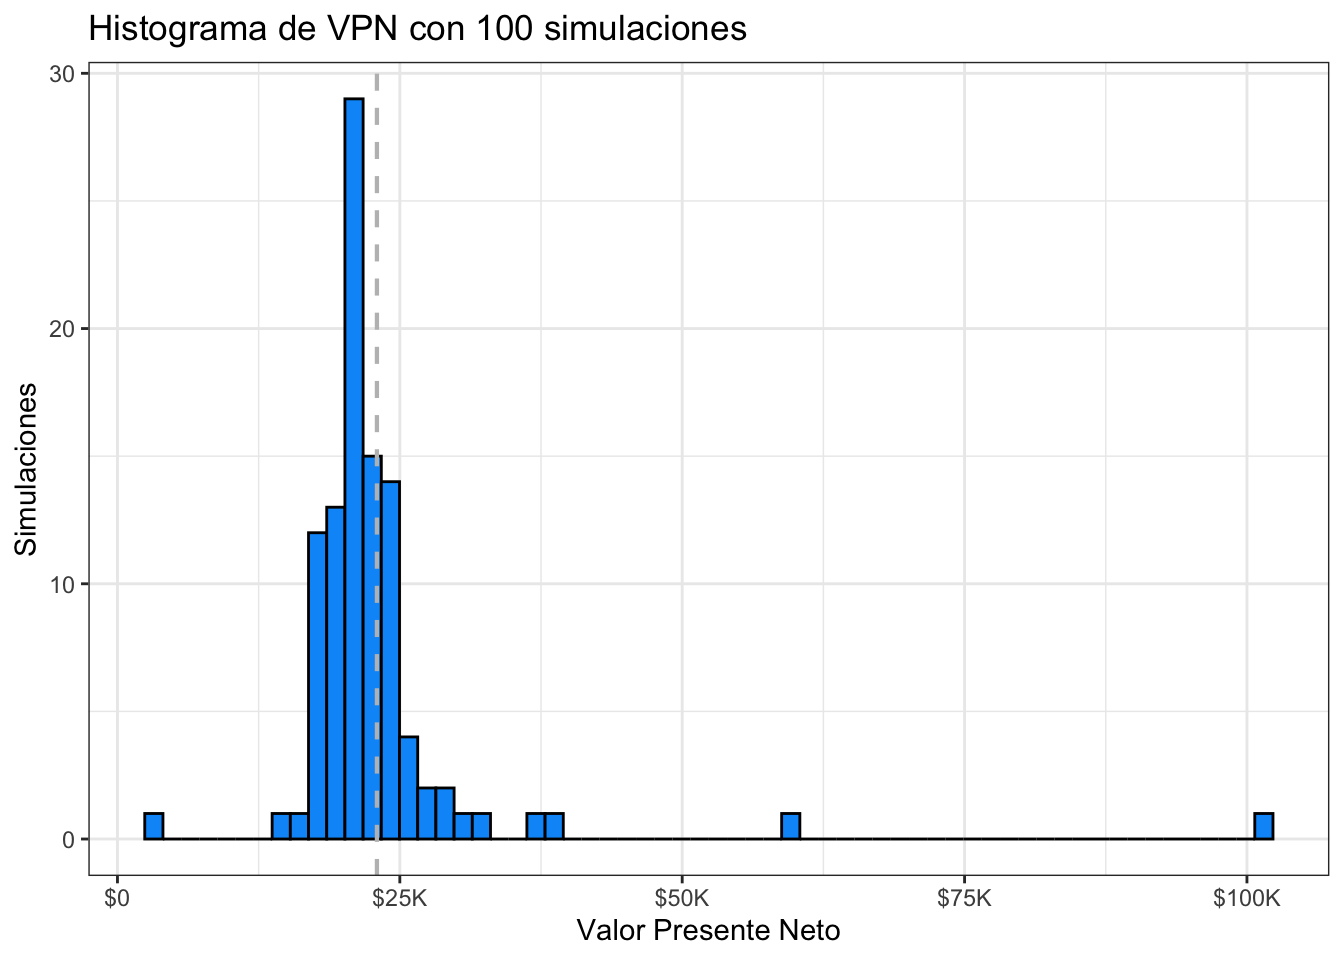
\includegraphics[width=0.65\linewidth]{_main_files/figure-latex/montetest5-1} 

}

\caption{Histograma de prueba de Monte Carlo}\label{fig:montetest5}
\end{figure}

Utilizando un número de
simulaciones igual a: 300, podemos observar los resultados en la Figura:
\ref{fig:montetest5}.

\newpage

\hypertarget{matriz-de-toma-de-decisiones-1}{%
\subsection{Matriz de Toma de Decisiones}\label{matriz-de-toma-de-decisiones-1}}

\textbf{{[}Agregar ejemplo de matriz de toma de decisiones{]}}

\newpage

\hypertarget{proceso-de-producciuxf3n-de-tabletas-personalizables}{%
\section{Proceso de Producción de Tabletas Personalizables}\label{proceso-de-producciuxf3n-de-tabletas-personalizables}}

El proceso de producción de las tabletas personalizables se puede
visualizar en la siguiente imagen:

\begin{figure}
\centering
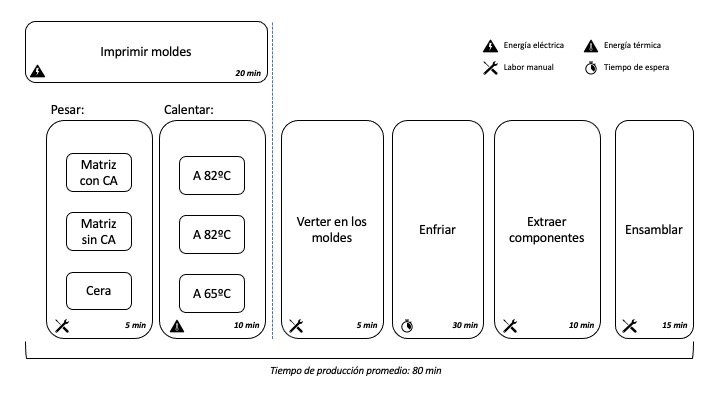
\includegraphics[width=0.9\textwidth,height=\textheight]{Diagramas/ProcesoProduccion.jpg}
\caption{Proceso de Producción de Tabletas
Personalizables}
\end{figure}

El componente de costos de la ecuación \eqref{eq:fcfeq} se puede expresar
de la siguiente manera:

\begin{equation}
  Costo = C_{Directo} + C_{Mantenimiento} \label{eq:costos}
\end{equation}

Cuyo componente de \(C_{Directo}\) es el resultado del producto del costo unitario
por el número de tabletas personalizables impresas en un el periodo:

\begin{equation}
  C_{Directo}=\left(C_{Material}+C_{Labor}+C_{Energia}+C_{Distribucion}\right)
  \times N_tabletas
  \label{eq:costodirecto}
\end{equation}

En donde:

\begin{itemize}
\item
  \(C_{Material}\) representa el costo de los materiales que constituyen
  la tableta, desde los componentes activos hasta la cera que los
  envuelve:

  \begin{equation}
  C_{Material}=\sum_{i=0}^n\left(m_i \times c_i \right) + C_{frasco}
  \label{eq:costomaterial}
  \end{equation}
\item
  \(C_{Labor}\) representa el costo de la mano de obra que conlleva
  realizar el proceso de producción:

  \begin{equation}
  C_{Labor}=\frac{t_{tableta}^{fabricacion} \times Salario_{trabajador}}
  {\eta_{trabajador}}
  \label{eq:costolabor}
  \end{equation}
\item
  \(C_{Energia}\) representa el costo energético de producción
  ocasionado por 1) el gasto energético de la impresora 3D
  (\(G_{impresora}^E\)) y 2) el gasto energético para el cambio de fase
  de los componentes \(G_{transicion}^E\) para vertirse en los moldes:
\end{itemize}

\begin{align}
  G_{impresora}^E & = t_{impresion} \times C_{impresora}^E \notag \\
  G_{transicion}^E & = \sum_{i=0}^n\left(m_i c_s\right)\Delta T_1 + 
  m_{cera}^{matrizCA}L_f^1 \notag \\
  & + \sum_{j=0}^m\left(m_j c_s\right)\Delta T_1 + m_{cera}^{matrizSCA}L_f^1
  \notag \\
  & + m_{cera}^{exterior} \times (c_s\Delta T_2 + L_f^2) \notag \\
  C_{Energia} & = \left(\frac{G_{transicion}^E}{\eta_{calentador}}
  +G_{impresora}^E \right) \times C_{electricidad} \label{eq:costoenergetico}
\end{align}

\begin{itemize}
\tightlist
\item
  \(C_D\) representa el costo de distribución de las tabletas el cual es
  resultado de la relación entre el tiempo de transporte, la distancia
  recorrida, el precio de la gasolina y el costo del trabajador
  necesario para transportar cierto número de tabletas:
\end{itemize}

    \begin{equation}
    C_D = \frac{t_{transporte} \times C_{trabajador} + \frac{Distancia \times 
    P_{gasolina}}{\eta_{vehiculo}}}{N_{tabletas}} 
    \label{eq:costodistribucion}
    \end{equation}

Mientras que el componente de ingresos de la ecuación \eqref{eq:fcfeq} se puede
expresar en función de los costos directos de la siguiente forma:

  \begin{equation}
  Ingresos = (1+MU) \times C_{Directo}
  \label{eq:ingresos}
  \end{equation}

En donde \(MU\) (\textbf{Markup}) es un número decimal que representa la cantidad
adicional sobre el costo de producción que estamos agregando al precio.

Con esta definición para el componente de ingresos, la ecuación \eqref{eq:fcfeq}
puede ser simplificada de la siguiente manera:

\begin{align}
  FCF & = (Ing. - Cost. - Depr.) \times (1-\tau_{c}) + Depr. - Inv. - \Delta CTN 
  \notag \\
  & = \left( \left((1 + MU) \times C_{Directo} \right) - 
  (C_{Directo} + C_{Mantenimiento})-Depr. \right)
  \times (1-\tau_{c}) + Depr. - Inv. - \Delta CTN \notag \\
  & = \left( \left(MU \times C_{Directo} \right) - C_{Mantenimiento} - Depr.
  \right)
  \times (1-\tau_{c}) + Depr. - Inv. - \Delta CTN
  \label{eq:fcfmod}
\end{align}

\hypertarget{composiciuxf3n-de-tabletas}{%
\subsection{Composición de tabletas}\label{composiciuxf3n-de-tabletas}}

La composición de las tabletas de formulación E1 es de 4\%-9\% de componente
activo y de 96\%-91\% de compuestos que forman la matriz (para la porción que
contiene el(los) compuesto(s) activo(s)). En la siguiente tabla podemos observar
la composición de la matriz:

\begin{verbatim}
## Rows: 3 Columns: 2
## -- Column specification -------------------------------------------------------------------------------
## Delimiter: ","
## chr (1): Compound
## dbl (1): Composicion_E1
## 
## i Use `spec()` to retrieve the full column specification for this data.
## i Specify the column types or set `show_col_types = FALSE` to quiet this message.
\end{verbatim}

\begin{table}

\caption{\label{tab:tabcomposicion}Composición de la matriz con formulación E1}
\centering
\begin{tabular}[t]{l|c}
\hline
Compuesto & \%\\
\hline
Sodium alginate & 0.42\\
\hline
Carnauba wax No. 1 yellow & 0.48\\
\hline
Croscarmellose Sodium & 0.10\\
\hline
\end{tabular}
\end{table}

\hypertarget{cuxe1lculo-de-material-necesario-para-moldes}{%
\section{Cálculo de material necesario para moldes}\label{cuxe1lculo-de-material-necesario-para-moldes}}

Para poder calcular la cantidad de ABS que va a ser necesario para imprimir los
moldes en los cuales se van a formar las piezas (o componentes) de las
tabletas personalizables, utilizamos una forma sencilla como base para la
geometría de los componentes. Podemos observar la geometría en la siguiente
figura:

\begin{figure}
\centering
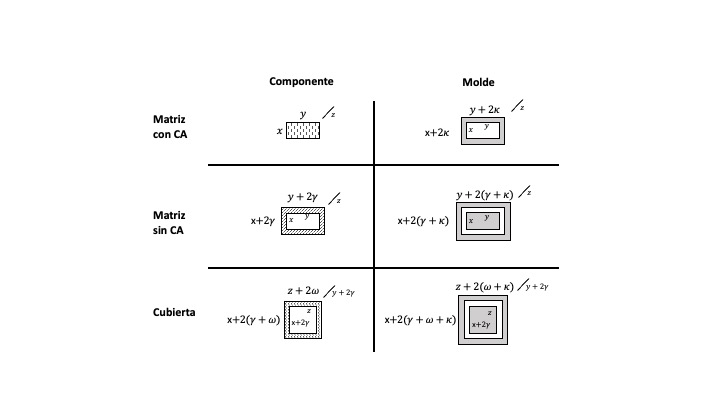
\includegraphics[width=0.9\textwidth,height=\textheight]{Diagramas/geometria_tabletas.jpg}
\caption{Geometría de los componentes de las tabletas y de sus moldes}
\end{figure}

\hypertarget{secuencia-de-cuxe1lculos}{%
\subsection{Secuencia de cálculos}\label{secuencia-de-cuxe1lculos}}

\begin{enumerate}
\def\labelenumi{\arabic{enumi}.}
\tightlist
\item
  Calcular el área transversal con base en \(z\), el ``ancho'' de la matriz
\item
  Calcular la masa de ABS necesaria para el primer molde \(m_{ABS}^{MACA}\)
\item
  Calcular el espesor de la cubierta de matriz sin compuesto activo \(\gamma\)
\item
  Calcular la masa de ABS necesaria para el segundo molde \(m_{ABS}^{MAS}\)
\item
  Calcular la masa de la cera necesaria para cubrir las dos matrices \(m_{cera}\)
\item
  Calcular la masa de ABS necesaria para el molde de la cubierta
  \(m_{ABS}^{cubierta}\)
\end{enumerate}

\hypertarget{variables}{%
\subsection{Variables}\label{variables}}

Para poder resolver el problema necesitamos reducir los grados de libertad del
mismo a través de la definición de las siguientes variables y o relaciones
entre variables:

\begin{enumerate}
\def\labelenumi{\alph{enumi}.}
\tightlist
\item
  El ancho de la matriz \(z\)
\item
  La relación entre \(x\) y \(y\)
\item
  El espesor de las paredes del molde \(\kappa\)
\item
  El espesor de la cubierta exterior de cera \(\omega\)
\end{enumerate}

\hypertarget{ecuaciones-para-la-resoluciuxf3n-del-problema}{%
\subsection{Ecuaciones para la resolución del problema}\label{ecuaciones-para-la-resoluciuxf3n-del-problema}}

\emph{Paso 1a}

\begin{equation}
A^{MACA}=\frac{\sum_{i=1}^n\left(m_i / \rho_i \right)}{z}
\end{equation}

\emph{Paso 1b}

\begin{align}
y &= 2x \notag \\
A^{MACA} &= x \times y = 3x \notag \\
x &= \frac{A^{MACA}}{3} \notag \\
y &= \frac{2}{3} \times A^{MACA} \notag
\end{align}

\emph{Paso 2}

\begin{align}
m_{ABS}^{MACA} & = \frac{V_{ABS}^{MACA}}{\rho_{ABS}} \notag \\
& = \frac{\left((x+2\kappa)(y+2\kappa) - (x \times y) \right) \times z}
{\rho_{ABS}} \notag \\
& = \frac{2\kappa\left(x+y+2\kappa \right) \times z}{\rho_{ABS}}
\end{align}

\emph{Paso 3}

\begin{align}
V^{MAS}&=\left( (x+2\gamma)(y+2\gamma)-x \times y \right) \times z \notag \\
V^{MAS}&=\sum_{j=1}^n(m_j / \rho_j) \notag \\
\sum_{j=1}^n(m_j / \rho_j) &= \left( (x+2\gamma)(y+2\gamma)-x \times y \right) 
\times z \notag \\
0 &= 4\gamma^2+2(x+y)\gamma-\frac{\sum_{j=1}^n(m_j / \rho_j)}{z} \label{eq:gamma}
\end{align}

Si observamos la ecuación \eqref{eq:gamma}, podemos observar que está en la
forma de la fórmula general \(x=\frac{-b\pm\sqrt{b^2-4ac}}{2a}\) en donde:

\begin{align}
a &= 4 \\
b &= 2(x+y) \\
c &= -\frac{\sum_{j=1}^n(m_j / \rho_j)}{z}
\end{align}

Con lo cual podemos calcular el valor de \(\gamma\):

\begin{align
\gamma &= \frac{-2(x+y)\pm\sqrt{\left(2(x+y)\right)^2-4(4) 
\left( -\frac{\sum_{j=1}^n(m_j / \rho_j)}{z}\right)}}{2(4)} \notag \\
 &= \frac{-2(x+y)\pm\sqrt{4(x+y)^2+16
\left(\frac{\sum_{j=1}^n(m_j / \rho_j)}{z}\right)}}{8} \label{eq:gamma1}
\end{align}

Dado que \(\gamma\) representa el espesor de las paredes de los moldes,
el resultado de la ecuación \eqref{eq:gamma1} debe de ser positivo. Así que la
ecuación se reduce a:

\begin{equation}
\gamma = \frac{-2(x+y)+\sqrt{4(x+y)^2+16
\left(\frac{\sum_{j=1}^n(m_j / \rho_j)}{z}\right)}}{8} \label{eq:gamma2}
\end{equation}

\emph{Paso 4}

\begin{align}
m_{ABS}&=\frac{V_{molde}^{MAS}}{\rho_{ABS}} \notag \\
V_{molde}^{MAS} &= \left[\left(x+2(\gamma+\kappa) \right)
\left(y+(\gamma+\kappa) \right)-V^{MAS} \right] \times z \label{eq:mpaso4}
\end{align}

\emph{Paso 5}

\begin{align}
m_{cera} &= \frac{V_{cera}}{\rho_{cera}} \notag \\
V_{cera} &= \left\{\left[x+2(\gamma+\omega)\right]\left[z+2\omega\right]-
(x+2\gamma)(z)\right\} \times (y+2\gamma) \notag \\
&= \left\{xz+2x\omega+2z(\gamma+\omega)+4\omega(\gamma+\omega)-xz-2z\gamma 
\right\} \times (y+2\gamma) \notag \\
&= \left\{2x\omega+2z\omega+4\omega(\gamma+\omega) \right\} 
\times (y+2\gamma) \notag \\
&= 2\omega \left\{x+z+2(\gamma+\omega) \right\} \times (y+2\gamma) \label{eq:vcera}
\end{align}

\emph{Paso 6}

\begin{align}
m_{ABS}^{cubierta} &=\frac{V_{molde}^{cubierta}}{\rho_{cera}} \notag \\
V_{molde}^{cubierta} &= \left\{\left[x+2(\gamma+\omega+\kappa) \right]\left[ 
z+2(\omega+\kappa\right] \right\} \times (y+2\gamma) \label{eq:vmoldecubierta}
\end{align}

\hypertarget{resultados}{%
\chapter{Resultados}\label{resultados}}

\hypertarget{datos-utilizados}{%
\section{Datos Utilizados}\label{datos-utilizados}}

\begin{verbatim}
## Rows: 7 Columns: 5
## -- Column specification -------------------------------------------------------------------------------
## Delimiter: ","
## chr (1): Compound
## dbl (4): Price_kg_usd, Specific_Heat, Fusion_Heat, Density
## 
## i Use `spec()` to retrieve the full column specification for this data.
## i Specify the column types or set `show_col_types = FALSE` to quiet this message.
\end{verbatim}

\begin{table}

\caption{\label{tab:tabinfocompuestos}Características y precio de los componentes}
\centering
\begin{tabular}[t]{l|c|c|c|c}
\hline
Compuestos & Calor Específico & Calor de Fusión & Densidad & Precio MXN/g\\
\hline
Sodium alginate & 1.5 & NA & 1.000 & 0.28\\
\hline
Carnauba wax No. 1 yellow & 2.1 & 168.59 & 0.990 & 0.01\\
\hline
Croscarmellose Sodium & 1.8 & NA & 0.480 & 0.33\\
\hline
Acetaminophen & 1.8 & NA & 1.300 & 1.60\\
\hline
Phenylephrine Hydrochloride & 1.8 & NA & 1.000 & 0.75\\
\hline
Diphenhydramine hydrochloride & 1.8 & NA & 1.013 & 0.15\\
\hline
White Wax & 2.1 & 165.47 & 0.958 & 0.05\\
\hline
\end{tabular}
\end{table}

La \ref{tab:tabinfocompuestos} muestra la información relacionada a los compuestos
utilizada para los cálculos de esta sección.

\hypertarget{costo-de-tabletas-unitario}{%
\section{Costo de tabletas unitario}\label{costo-de-tabletas-unitario}}

\hypertarget{componente-de-material}{%
\subsection{Componente de material}\label{componente-de-material}}

\hypertarget{componente-de-labor}{%
\subsection{Componente de labor}\label{componente-de-labor}}

\hypertarget{componente-de-energuxeda}{%
\subsection{Componente de energía}\label{componente-de-energuxeda}}

\hypertarget{componente-de-distribuciuxf3n}{%
\subsection{Componente de distribución}\label{componente-de-distribuciuxf3n}}

\hypertarget{costo-de-inversiuxf3n}{%
\section{Costo de inversión}\label{costo-de-inversiuxf3n}}

\hypertarget{depreciaciuxf3n}{%
\section{Depreciación}\label{depreciaciuxf3n}}

\hypertarget{discusion}{%
\chapter{Discusion}\label{discusion}}

\hypertarget{conclusiones}{%
\chapter{Conclusiones}\label{conclusiones}}

Aquí van a ir las conclusiones del trabajo.

\hypertarget{apendice}{%
\chapter{Apendice}\label{apendice}}

El siguiente código forma parte del cuerpo del trabajo:

\begin{Shaded}
\begin{Highlighting}[]
\CommentTok{\# Setup chunk: Carga los paquetes necesarios para realizar los cálculos en }
\CommentTok{\# lo que resta del trabajo }

\ControlFlowTok{if}\NormalTok{ (}\SpecialCharTok{!}\FunctionTok{require}\NormalTok{(}\StringTok{"pacman"}\NormalTok{)) }\FunctionTok{install.packages}\NormalTok{(}\StringTok{"pacman"}\NormalTok{)}
\NormalTok{pacman}\SpecialCharTok{::}\FunctionTok{p\_load}\NormalTok{(tidyverse, EnvStats, knitr, scales, formattable)}

\NormalTok{rversion }\OtherTok{\textless{}{-}}\NormalTok{ R.version.string}
\FunctionTok{sessionInfo}\NormalTok{()}

\CommentTok{\# El siguiente código es para crear una gráfica de tornado ejemplo}
\CommentTok{\# El código que crea la gráfica se encuentra en el archivo que se carga a }
\CommentTok{\# continuación. Éste se puede encontrar más adelante en el apéndice}
\FunctionTok{source}\NormalTok{(}\StringTok{"Scripts/SensitivityAnalysis.R"}\NormalTok{, }\AttributeTok{local =}\NormalTok{ knitr}\SpecialCharTok{::}\FunctionTok{knit\_global}\NormalTok{())}

  \FunctionTok{set.seed}\NormalTok{(}\DecValTok{1}\NormalTok{)}
  \FunctionTok{tornado}\NormalTok{(}\FunctionTok{sensitivity}\NormalTok{()) }\SpecialCharTok{+} 
    \FunctionTok{labs}\NormalTok{(}\AttributeTok{title =} \StringTok{"Gráfica Tornado Ilustrativa"}\NormalTok{,}
    \AttributeTok{subtitle =} \StringTok{"Utilizando 12 valores aleatorios"}\NormalTok{,}
    \AttributeTok{caption =} \StringTok{""}\NormalTok{,}
    \AttributeTok{fill =} \StringTok{""}\NormalTok{,}
    \AttributeTok{x =} \StringTok{"Valor Presente Neto"}\NormalTok{, }\AttributeTok{y =} \StringTok{"Variable"}\NormalTok{)}


\CommentTok{\# Este chunk crea y muestra la tabla de criterios para utilizar en la matriz}
\CommentTok{\# de toma de decisiones}

\NormalTok{Criterio }\OtherTok{\textless{}{-}} \FunctionTok{c}\NormalTok{(}\StringTok{"VPN"}\NormalTok{,}\StringTok{"Beneficio Social"}\NormalTok{,}\StringTok{"Impacto Ambiental"}\NormalTok{)}
\NormalTok{VPN }\OtherTok{\textless{}{-}} \FunctionTok{c}\NormalTok{(}\StringTok{"1"}\NormalTok{,}\StringTok{"2"}\NormalTok{,}\StringTok{"4"}\NormalTok{)}
\NormalTok{Beneficio.Social }\OtherTok{\textless{}{-}} \FunctionTok{c}\NormalTok{(}\StringTok{"1/2"}\NormalTok{,}\StringTok{"1"}\NormalTok{,}\StringTok{"2"}\NormalTok{)}
\NormalTok{Impacto.Ambiental }\OtherTok{\textless{}{-}} \FunctionTok{c}\NormalTok{(}\StringTok{"1/4"}\NormalTok{,}\StringTok{"1/2"}\NormalTok{,}\StringTok{"1"}\NormalTok{)}
\NormalTok{df }\OtherTok{\textless{}{-}} \FunctionTok{cbind}\NormalTok{(Criterio, VPN,Beneficio.Social,Impacto.Ambiental)}
\NormalTok{df }\OtherTok{\textless{}{-}} \FunctionTok{as.data.frame}\NormalTok{(df)}

\NormalTok{knitr}\SpecialCharTok{::}\FunctionTok{kable}\NormalTok{(df, }\AttributeTok{col.names =} \FunctionTok{gsub}\NormalTok{(}\StringTok{"[.]"}\NormalTok{, }\StringTok{" "}\NormalTok{, }\FunctionTok{names}\NormalTok{(df)), }
             \AttributeTok{caption =} \StringTok{"Comparativo del valor de los criterios (AHP)"}\NormalTok{, }
             \AttributeTok{align =} \StringTok{"lccc"}\NormalTok{)}


\NormalTok{test\_df }\OtherTok{\textless{}{-}} \FunctionTok{tibble}\NormalTok{(}
  \AttributeTok{periods =} \DecValTok{0}\SpecialCharTok{:}\DecValTok{10}\NormalTok{,}
  \AttributeTok{cashflow =} \FunctionTok{c}\NormalTok{(}\SpecialCharTok{{-}}\DecValTok{5000}\NormalTok{,}\FunctionTok{rep}\NormalTok{(}\DecValTok{1000}\NormalTok{,}\DecValTok{10}\NormalTok{))}
\NormalTok{)}

\NormalTok{test\_df}\SpecialCharTok{$}\NormalTok{cashflow }\OtherTok{\textless{}{-}} \FunctionTok{currency}\NormalTok{(test\_df}\SpecialCharTok{$}\NormalTok{cashflow, }\AttributeTok{digits =}\NormalTok{ 0L)}

\NormalTok{knitr}\SpecialCharTok{::}\FunctionTok{kable}\NormalTok{(test\_df, }\AttributeTok{col.names =} \FunctionTok{gsub}\NormalTok{(}\StringTok{"[.]"}\NormalTok{, }\StringTok{" "}\NormalTok{, }\FunctionTok{names}\NormalTok{(test\_df)), }
             \AttributeTok{caption =} 
               \StringTok{"Flujos de efectivo de prueba"}\NormalTok{, }
             \AttributeTok{align =} \StringTok{"lccc"}\NormalTok{)}

  \CommentTok{\# Cargar función de Valor Presente Neto}
  \FunctionTok{source}\NormalTok{(}\StringTok{"scripts/funciones\_financieras.R"}\NormalTok{, }\AttributeTok{local =}\NormalTok{ knitr}\SpecialCharTok{::}\FunctionTok{knit\_global}\NormalTok{())}

\NormalTok{  rate }\OtherTok{\textless{}{-}} \FloatTok{0.08}
\NormalTok{  test\_npv }\OtherTok{\textless{}{-}} 
  \FunctionTok{npv}\NormalTok{(}\AttributeTok{rate =}\NormalTok{ rate, }\AttributeTok{cashflow =}\NormalTok{ test\_df}\SpecialCharTok{$}\NormalTok{cashflow, }\AttributeTok{period =}\NormalTok{ test\_df}\SpecialCharTok{$}\NormalTok{periods)}
  
\NormalTok{  test\_npv }\OtherTok{\textless{}{-}} \FunctionTok{currency}\NormalTok{(test\_npv, }\AttributeTok{digits =}\NormalTok{ 2L)}
\CommentTok{\# Definir los costos de implementación}
\NormalTok{lowImpCost }\OtherTok{\textless{}{-}} \DecValTok{10000}
\NormalTok{highImpCost }\OtherTok{\textless{}{-}} \DecValTok{20000}

\CommentTok{\# Definir los costos de electricidad}
\NormalTok{lowElecCost }\OtherTok{\textless{}{-}} \DecValTok{50}
\NormalTok{highElecCost }\OtherTok{\textless{}{-}} \DecValTok{100}

\CommentTok{\# Definir uso de electricidad}
\NormalTok{withImp }\OtherTok{\textless{}{-}} \DecValTok{500}
\NormalTok{noImp }\OtherTok{\textless{}{-}} \DecValTok{800}

\CommentTok{\# Definir periodo de evaluación en años}
\NormalTok{emv\_test\_n }\OtherTok{\textless{}{-}} \DecValTok{10}
\NormalTok{emv\_test\_rate }\OtherTok{\textless{}{-}} \FloatTok{0.06}


\CommentTok{\# Crear un data frame con los valores especificados en el chunk anterior}
\NormalTok{Variable }\OtherTok{\textless{}{-}} \FunctionTok{c}\NormalTok{(}\StringTok{"Costo Implementación"}\NormalTok{,}\StringTok{"Costo Electricidad"}\NormalTok{)}
\NormalTok{Alto }\OtherTok{\textless{}{-}} \FunctionTok{c}\NormalTok{(highImpCost, highElecCost)}
\NormalTok{Bajo }\OtherTok{\textless{}{-}} \FunctionTok{c}\NormalTok{(lowImpCost, lowElecCost)}
\NormalTok{emv\_test\_df }\OtherTok{\textless{}{-}} \FunctionTok{cbind}\NormalTok{(Variable, Alto, Bajo)}
\NormalTok{emv\_test\_df }\OtherTok{\textless{}{-}} \FunctionTok{as.data.frame}\NormalTok{(emv\_test\_df)}

\CommentTok{\# Dar formato de moneda}
\NormalTok{emv\_test\_df}\SpecialCharTok{$}\NormalTok{Alto }\OtherTok{\textless{}{-}} \FunctionTok{currency}\NormalTok{(emv\_test\_df}\SpecialCharTok{$}\NormalTok{Alto, }\AttributeTok{symbol =} \StringTok{"$"}\NormalTok{, }\AttributeTok{digits =}\NormalTok{ 0L)}
\NormalTok{emv\_test\_df}\SpecialCharTok{$}\NormalTok{Bajo }\OtherTok{\textless{}{-}} \FunctionTok{currency}\NormalTok{(emv\_test\_df}\SpecialCharTok{$}\NormalTok{Bajo, }\AttributeTok{symbol =} \StringTok{"$"}\NormalTok{, }\AttributeTok{digits =}\NormalTok{ 0L)}

\CommentTok{\# Dar formato de tabla usando knitr}
\NormalTok{knitr}\SpecialCharTok{::}\FunctionTok{kable}\NormalTok{(emv\_test\_df, }\AttributeTok{col.names =} \FunctionTok{gsub}\NormalTok{(}\StringTok{"[.]"}\NormalTok{, }\StringTok{" "}\NormalTok{, }\FunctionTok{names}\NormalTok{(emv\_test\_df)), }
             \AttributeTok{caption =} \StringTok{"Valores para prueba de funcionamiento de EMV"}\NormalTok{, }
             \AttributeTok{align =} \StringTok{"lccc"}\NormalTok{)}


\FunctionTok{library}\NormalTok{(data.tree)}
\FunctionTok{library}\NormalTok{(DiagrammeR)}
\FunctionTok{library}\NormalTok{(webshot)}

\NormalTok{invest }\OtherTok{\textless{}{-}}\NormalTok{ Node}\SpecialCharTok{$}\FunctionTok{new}\NormalTok{(}\StringTok{"Invertir?"}\NormalTok{, }\AttributeTok{type =} \StringTok{"decision"}\NormalTok{)}
\NormalTok{  yes }\OtherTok{\textless{}{-}}\NormalTok{ invest}\SpecialCharTok{$}\FunctionTok{AddChild}\NormalTok{(}\StringTok{"Si"}\NormalTok{, }\AttributeTok{type =} \StringTok{"chance"}\NormalTok{)}
\NormalTok{    lowImplementation }\OtherTok{\textless{}{-}} 
\NormalTok{      yes}\SpecialCharTok{$}\FunctionTok{AddChild}\NormalTok{(}\StringTok{"Costo Bajo de Implementacion"}\NormalTok{, }\AttributeTok{type =} \StringTok{"chance"}\NormalTok{)}
\NormalTok{      lowHigh }\OtherTok{\textless{}{-}} 
\NormalTok{        lowImplementation}\SpecialCharTok{$}\FunctionTok{AddChild}\NormalTok{(}\StringTok{"Costo Alto de Electricidad"}\NormalTok{, }\AttributeTok{type =} \StringTok{"terminal"}\NormalTok{)}
\NormalTok{      lowLow }\OtherTok{\textless{}{-}} 
\NormalTok{        lowImplementation}\SpecialCharTok{$}\FunctionTok{AddChild}\NormalTok{(}\StringTok{"Costo Bajo de Electricidad"}\NormalTok{, }\AttributeTok{type =} \StringTok{"terminal"}\NormalTok{)}
\NormalTok{    highImplementation }\OtherTok{\textless{}{-}} 
\NormalTok{      yes}\SpecialCharTok{$}\FunctionTok{AddChild}\NormalTok{(}\StringTok{"Costo Alto de Implementacion"}\NormalTok{, }\AttributeTok{type =} \StringTok{"chance"}\NormalTok{)}
\NormalTok{      highHigh }\OtherTok{\textless{}{-}} 
\NormalTok{        highImplementation}\SpecialCharTok{$}\FunctionTok{AddChild}\NormalTok{(}\StringTok{"1 Costo Alto de Electricidad"}\NormalTok{, }
                                    \AttributeTok{type =} \StringTok{"terminal"}\NormalTok{)}
\NormalTok{      highLow }\OtherTok{\textless{}{-}} 
\NormalTok{        highImplementation}\SpecialCharTok{$}\FunctionTok{AddChild}\NormalTok{(}\StringTok{"1 Costo Bajo de Electricidad"}\NormalTok{, }
                                    \AttributeTok{type =} \StringTok{"terminal"}\NormalTok{)}
\NormalTok{  no }\OtherTok{\textless{}{-}}\NormalTok{ invest}\SpecialCharTok{$}\FunctionTok{AddChild}\NormalTok{(}\StringTok{"No"}\NormalTok{, }\AttributeTok{type =} \StringTok{"chance"}\NormalTok{)}
\NormalTok{    noHigh }\OtherTok{\textless{}{-}}\NormalTok{ no}\SpecialCharTok{$}\FunctionTok{AddChild}\NormalTok{(}\StringTok{"2 Costo Alto de Electricidad"}\NormalTok{, }\AttributeTok{type =} \StringTok{"terminal"}\NormalTok{)}
\NormalTok{    noLow }\OtherTok{\textless{}{-}}\NormalTok{ no}\SpecialCharTok{$}\FunctionTok{AddChild}\NormalTok{(}\StringTok{"2 Costo Bajo de Electricidad"}\NormalTok{, }\AttributeTok{type =} \StringTok{"terminal"}\NormalTok{)}

\CommentTok{\# Cargar funciones de arboles}
\FunctionTok{source}\NormalTok{(}\StringTok{"scripts/tree\_functions.R"}\NormalTok{, }\AttributeTok{local =}\NormalTok{ knitr}\SpecialCharTok{::}\FunctionTok{knit\_global}\NormalTok{())    }
    
\FunctionTok{SetGraphStyle}\NormalTok{(invest, }\AttributeTok{rankdir =} \StringTok{"TB"}\NormalTok{)}
\FunctionTok{SetNodeStyle}\NormalTok{(invest, }\AttributeTok{style =} \StringTok{"filled,rounded"}\NormalTok{, }
             \AttributeTok{label =}\NormalTok{ AdjustNodeName, }\AttributeTok{shape =} \StringTok{"box"}\NormalTok{)}

\FunctionTok{plot}\NormalTok{(invest)}


\CommentTok{\# Agregar valores de probabilidad a cada uno de nodos de casualidad}
\NormalTok{invest}\SpecialCharTok{$}\NormalTok{Si}\SpecialCharTok{$}\StringTok{\textasciigrave{}}\AttributeTok{Costo Bajo de Implementacion}\StringTok{\textasciigrave{}}\SpecialCharTok{$}\NormalTok{prob }\OtherTok{\textless{}{-}} \FloatTok{0.5}
\NormalTok{invest}\SpecialCharTok{$}\NormalTok{Si}\SpecialCharTok{$}\StringTok{\textasciigrave{}}\AttributeTok{Costo Bajo de Implementacion}\StringTok{\textasciigrave{}}\SpecialCharTok{$}\StringTok{\textasciigrave{}}\AttributeTok{Costo Alto de Electricidad}\StringTok{\textasciigrave{}}\SpecialCharTok{$}\NormalTok{prob }\OtherTok{\textless{}{-}} \FloatTok{0.6}
\NormalTok{invest}\SpecialCharTok{$}\NormalTok{Si}\SpecialCharTok{$}\StringTok{\textasciigrave{}}\AttributeTok{Costo Bajo de Implementacion}\StringTok{\textasciigrave{}}\SpecialCharTok{$}\StringTok{\textasciigrave{}}\AttributeTok{Costo Bajo de Electricidad}\StringTok{\textasciigrave{}}\SpecialCharTok{$}\NormalTok{prob }\OtherTok{\textless{}{-}} \FloatTok{0.4}
\NormalTok{invest}\SpecialCharTok{$}\NormalTok{Si}\SpecialCharTok{$}\StringTok{\textasciigrave{}}\AttributeTok{Costo Alto de Implementacion}\StringTok{\textasciigrave{}}\SpecialCharTok{$}\NormalTok{prob }\OtherTok{\textless{}{-}} \FloatTok{0.5}
\NormalTok{invest}\SpecialCharTok{$}\NormalTok{Si}\SpecialCharTok{$}\StringTok{\textasciigrave{}}\AttributeTok{Costo Alto de Implementacion}\StringTok{\textasciigrave{}}\SpecialCharTok{$}\StringTok{\textasciigrave{}}\AttributeTok{1 Costo Alto de Electricidad}\StringTok{\textasciigrave{}}\SpecialCharTok{$}\NormalTok{prob }\OtherTok{\textless{}{-}} \FloatTok{0.6}
\NormalTok{invest}\SpecialCharTok{$}\NormalTok{Si}\SpecialCharTok{$}\StringTok{\textasciigrave{}}\AttributeTok{Costo Alto de Implementacion}\StringTok{\textasciigrave{}}\SpecialCharTok{$}\StringTok{\textasciigrave{}}\AttributeTok{1 Costo Bajo de Electricidad}\StringTok{\textasciigrave{}}\SpecialCharTok{$}\NormalTok{prob }\OtherTok{\textless{}{-}} \FloatTok{0.4}
\NormalTok{invest}\SpecialCharTok{$}\NormalTok{No}\SpecialCharTok{$}\StringTok{\textasciigrave{}}\AttributeTok{2 Costo Alto de Electricidad}\StringTok{\textasciigrave{}}\SpecialCharTok{$}\NormalTok{prob }\OtherTok{\textless{}{-}} \FloatTok{0.6}
\NormalTok{invest}\SpecialCharTok{$}\NormalTok{No}\SpecialCharTok{$}\StringTok{\textasciigrave{}}\AttributeTok{2 Costo Bajo de Electricidad}\StringTok{\textasciigrave{}}\SpecialCharTok{$}\NormalTok{prob }\OtherTok{\textless{}{-}} \FloatTok{0.4}

\CommentTok{\# Darle formato de porcentaje}
\FunctionTok{SetFormat}\NormalTok{(invest, }\StringTok{"prob"}\NormalTok{, }\AttributeTok{formatFun =}\NormalTok{ FormatPercent)}

\CommentTok{\# Cargar funcion de Valor Presente Neto}
\FunctionTok{source}\NormalTok{(}\StringTok{"scripts/funciones\_financieras.R"}\NormalTok{, }\AttributeTok{local =}\NormalTok{ knitr}\SpecialCharTok{::}\FunctionTok{knit\_global}\NormalTok{())}
\FunctionTok{source}\NormalTok{(}\StringTok{"scripts/valorMonetarioEsperado.R"}\NormalTok{, }\AttributeTok{local =}\NormalTok{ knitr}\SpecialCharTok{::}\FunctionTok{knit\_global}\NormalTok{())}

\CommentTok{\# Calcular los costos para los escenarios}
\NormalTok{low\_elect\_per }\OtherTok{\textless{}{-}} \FunctionTok{rep}\NormalTok{(lowElecCost, emv\_test\_n)}
\NormalTok{high\_elect\_per }\OtherTok{\textless{}{-}} \FunctionTok{rep}\NormalTok{(highElecCost, emv\_test\_n)}
\NormalTok{low\_imp\_per }\OtherTok{\textless{}{-}} \FunctionTok{c}\NormalTok{(lowImpCost, }\FunctionTok{rep}\NormalTok{(}\DecValTok{0}\NormalTok{, emv\_test\_n }\SpecialCharTok{{-}} \DecValTok{1}\NormalTok{))}
\NormalTok{high\_imp\_per }\OtherTok{\textless{}{-}} \FunctionTok{c}\NormalTok{(highImpCost, }\FunctionTok{rep}\NormalTok{(}\DecValTok{0}\NormalTok{, emv\_test\_n }\SpecialCharTok{{-}} \DecValTok{1}\NormalTok{))}
\NormalTok{emv\_test\_period }\OtherTok{\textless{}{-}} \DecValTok{0}\SpecialCharTok{:}\NormalTok{(emv\_test\_n}\DecValTok{{-}1}\NormalTok{)}

\CommentTok{\# Calcular valores de NPV para los nodos finales}
\NormalTok{invest}\SpecialCharTok{$}\NormalTok{Si}\SpecialCharTok{$}\StringTok{\textasciigrave{}}\AttributeTok{Costo Bajo de Implementacion}\StringTok{\textasciigrave{}}\SpecialCharTok{$}\StringTok{\textasciigrave{}}\AttributeTok{Costo Alto de Electricidad}\StringTok{\textasciigrave{}}\SpecialCharTok{$}\NormalTok{npv }\OtherTok{\textless{}{-}} 
  \FunctionTok{npv}\NormalTok{(emv\_test\_rate, }\SpecialCharTok{{-}}\NormalTok{(low\_imp\_per}\SpecialCharTok{+}\NormalTok{high\_elect\_per}\SpecialCharTok{*}\NormalTok{withImp), emv\_test\_period)}
\NormalTok{invest}\SpecialCharTok{$}\NormalTok{Si}\SpecialCharTok{$}\StringTok{\textasciigrave{}}\AttributeTok{Costo Bajo de Implementacion}\StringTok{\textasciigrave{}}\SpecialCharTok{$}\StringTok{\textasciigrave{}}\AttributeTok{Costo Bajo de Electricidad}\StringTok{\textasciigrave{}}\SpecialCharTok{$}\NormalTok{npv }\OtherTok{\textless{}{-}}
  \FunctionTok{npv}\NormalTok{(emv\_test\_rate, }\SpecialCharTok{{-}}\NormalTok{(low\_imp\_per}\SpecialCharTok{+}\NormalTok{low\_elect\_per}\SpecialCharTok{*}\NormalTok{withImp), emv\_test\_period)}
\NormalTok{invest}\SpecialCharTok{$}\NormalTok{Si}\SpecialCharTok{$}\StringTok{\textasciigrave{}}\AttributeTok{Costo Alto de Implementacion}\StringTok{\textasciigrave{}}\SpecialCharTok{$}\StringTok{\textasciigrave{}}\AttributeTok{1 Costo Alto de Electricidad}\StringTok{\textasciigrave{}}\SpecialCharTok{$}\NormalTok{npv }\OtherTok{\textless{}{-}}
  \FunctionTok{npv}\NormalTok{(emv\_test\_rate, }\SpecialCharTok{{-}}\NormalTok{(high\_imp\_per}\SpecialCharTok{+}\NormalTok{high\_elect\_per}\SpecialCharTok{*}\NormalTok{withImp), emv\_test\_period)}
\NormalTok{invest}\SpecialCharTok{$}\NormalTok{Si}\SpecialCharTok{$}\StringTok{\textasciigrave{}}\AttributeTok{Costo Alto de Implementacion}\StringTok{\textasciigrave{}}\SpecialCharTok{$}\StringTok{\textasciigrave{}}\AttributeTok{1 Costo Bajo de Electricidad}\StringTok{\textasciigrave{}}\SpecialCharTok{$}\NormalTok{npv }\OtherTok{\textless{}{-}}
  \FunctionTok{npv}\NormalTok{(emv\_test\_rate, }\SpecialCharTok{{-}}\NormalTok{(high\_imp\_per}\SpecialCharTok{+}\NormalTok{low\_elect\_per}\SpecialCharTok{*}\NormalTok{withImp), emv\_test\_period)}
\NormalTok{invest}\SpecialCharTok{$}\NormalTok{No}\SpecialCharTok{$}\StringTok{\textasciigrave{}}\AttributeTok{2 Costo Alto de Electricidad}\StringTok{\textasciigrave{}}\SpecialCharTok{$}\NormalTok{npv }\OtherTok{\textless{}{-}}
  \FunctionTok{npv}\NormalTok{(emv\_test\_rate, }\SpecialCharTok{{-}}\NormalTok{(high\_elect\_per}\SpecialCharTok{*}\NormalTok{noImp), emv\_test\_period)}
\NormalTok{invest}\SpecialCharTok{$}\NormalTok{No}\SpecialCharTok{$}\StringTok{\textasciigrave{}}\AttributeTok{2 Costo Bajo de Electricidad}\StringTok{\textasciigrave{}}\SpecialCharTok{$}\NormalTok{npv }\OtherTok{\textless{}{-}}
  \FunctionTok{npv}\NormalTok{(emv\_test\_rate, }\SpecialCharTok{{-}}\NormalTok{(low\_elect\_per}\SpecialCharTok{*}\NormalTok{noImp), emv\_test\_period)}

\CommentTok{\# Calcular los valores de NPV para los nodos de decision}


\NormalTok{invest}\SpecialCharTok{$}\FunctionTok{Do}\NormalTok{(}\ControlFlowTok{function}\NormalTok{(node) node}\SpecialCharTok{$}\NormalTok{npv }\OtherTok{\textless{}{-}} 
            \FunctionTok{w\_npv}\NormalTok{(node), }\AttributeTok{filterFun =}\NormalTok{ isNotLeaf, }\AttributeTok{traversal =} \StringTok{"post{-}order"}\NormalTok{)}

\CommentTok{\# Convertir a dataframe para visualizar}
\NormalTok{df }\OtherTok{\textless{}{-}} \FunctionTok{ToDataFrameTree}\NormalTok{(invest, }\StringTok{"prob"}\NormalTok{, }\StringTok{"npv"}\NormalTok{)}

\CommentTok{\# Cambiar formato}
\NormalTok{df}\SpecialCharTok{$}\NormalTok{npv[df}\SpecialCharTok{$}\NormalTok{levelName }\SpecialCharTok{==} \StringTok{"Invertir?                            "}\NormalTok{] }\OtherTok{\textless{}{-}} \ConstantTok{NA}
\NormalTok{df}\SpecialCharTok{$}\NormalTok{npv }\OtherTok{\textless{}{-}} \FunctionTok{currency}\NormalTok{(df}\SpecialCharTok{$}\NormalTok{npv, }\AttributeTok{symbol =} \StringTok{"$"}\NormalTok{, }\AttributeTok{digits =}\NormalTok{ 0L)}
\NormalTok{df}\SpecialCharTok{$}\NormalTok{prob }\OtherTok{\textless{}{-}} \FunctionTok{percent}\NormalTok{(df}\SpecialCharTok{$}\NormalTok{prob)}


\CommentTok{\# Mostrar como table usando knitr}
\NormalTok{knitr}\SpecialCharTok{::}\FunctionTok{kable}\NormalTok{(df, }\AttributeTok{col.names =} \FunctionTok{c}\NormalTok{(}\StringTok{"Nivel"}\NormalTok{, }\StringTok{"Probabilidad"}\NormalTok{, }\StringTok{"NVP"}\NormalTok{), }
             \AttributeTok{caption =} \StringTok{"Resultados de prueba de Valor Monetario Esperado"}\NormalTok{, }
             \AttributeTok{align =} \StringTok{"lccc"}\NormalTok{)}



\FunctionTok{library}\NormalTok{(data.tree)}
\FunctionTok{library}\NormalTok{(DiagrammeR)}
\FunctionTok{library}\NormalTok{(webshot)}

\CommentTok{\# Cargar funciones de arboles}
\FunctionTok{source}\NormalTok{(}\StringTok{"scripts/tree\_functions.R"}\NormalTok{, }\AttributeTok{local =}\NormalTok{ knitr}\SpecialCharTok{::}\FunctionTok{knit\_global}\NormalTok{())}

\FunctionTok{PlotDecisionTree}\NormalTok{(invest)}

\CommentTok{\# Generar valores base}
\NormalTok{base\_case }\OtherTok{\textless{}{-}} \FunctionTok{tibble}\NormalTok{(}
  \AttributeTok{variable =} 
    \FunctionTok{c}\NormalTok{(}\StringTok{"Inversion.Capital"}\NormalTok{, }\StringTok{"Gasto.Anual"}\NormalTok{, }\StringTok{"Ahorro.Anual"}\NormalTok{, }\StringTok{"TMAR"}\NormalTok{, }\StringTok{"Periodo"}\NormalTok{),}
  \AttributeTok{valor =} \FunctionTok{c}\NormalTok{(}\DecValTok{1100000}\NormalTok{, }\DecValTok{200000}\NormalTok{, }\DecValTok{500000}\NormalTok{, }\FloatTok{0.1}\NormalTok{, }\DecValTok{5}\NormalTok{)}
\NormalTok{)}

\CommentTok{\# Cambiar formato}
\NormalTok{print\_base }\OtherTok{\textless{}{-}}\NormalTok{ base\_case}
\NormalTok{print\_base}\SpecialCharTok{$}\NormalTok{valor }\OtherTok{\textless{}{-}} \FunctionTok{currency}\NormalTok{(print\_base}\SpecialCharTok{$}\NormalTok{valor, }\AttributeTok{symbol =} \StringTok{""}\NormalTok{, }\AttributeTok{digits =}\NormalTok{ 2L)}

\CommentTok{\# Mostrar como tabla usando knitr}
\NormalTok{knitr}\SpecialCharTok{::}\FunctionTok{kable}\NormalTok{(print\_base, }\AttributeTok{col.names =} \FunctionTok{gsub}\NormalTok{(}\StringTok{"[.]"}\NormalTok{, }\StringTok{" "}\NormalTok{, }\FunctionTok{names}\NormalTok{(print\_base)), }
             \AttributeTok{caption =} \StringTok{"Valores de caso base para prueba de Análisis de Sensibilidad"}\NormalTok{, }
             \AttributeTok{align =} \StringTok{"lccc"}\NormalTok{)}

\CommentTok{\# Calcular caso base contra lo cual se van a comparar los demás resultados}

\NormalTok{ult\_periodo }\OtherTok{=}\NormalTok{ base\_case}\SpecialCharTok{$}\NormalTok{valor[base\_case}\SpecialCharTok{$}\NormalTok{variable }\SpecialCharTok{==} \StringTok{"Periodo"}\NormalTok{]}

\NormalTok{base\_tib }\OtherTok{\textless{}{-}} \FunctionTok{tibble}\NormalTok{(}
  \AttributeTok{periodo =} \FunctionTok{c}\NormalTok{(}\DecValTok{0}\SpecialCharTok{:}\NormalTok{(ult\_periodo }\SpecialCharTok{{-}} \DecValTok{1}\NormalTok{)),}
  \AttributeTok{cashflow =} \FunctionTok{c}\NormalTok{(}\SpecialCharTok{{-}}\NormalTok{base\_case}\SpecialCharTok{$}\NormalTok{valor[base\_case}\SpecialCharTok{$}\NormalTok{variable }\SpecialCharTok{==} \StringTok{"Inversion.Capital"}\NormalTok{], }
      \FunctionTok{rep}\NormalTok{(}\DecValTok{0}\NormalTok{, ult\_periodo }\SpecialCharTok{{-}} \DecValTok{1}\NormalTok{)) }\SpecialCharTok{+}
\NormalTok{    (}\FunctionTok{rep}\NormalTok{(base\_case}\SpecialCharTok{$}\NormalTok{valor[base\_case}\SpecialCharTok{$}\NormalTok{variable }\SpecialCharTok{==} \StringTok{"Ahorro.Anual"}\NormalTok{], ult\_periodo) }\SpecialCharTok{{-}}
       \FunctionTok{rep}\NormalTok{(base\_case}\SpecialCharTok{$}\NormalTok{valor[base\_case}\SpecialCharTok{$}\NormalTok{variable }\SpecialCharTok{==} \StringTok{"Gasto.Anual"}\NormalTok{], ult\_periodo))}
\NormalTok{)}

\NormalTok{base\_npv }\OtherTok{\textless{}{-}} \FunctionTok{npv}\NormalTok{(}\AttributeTok{rate =}\NormalTok{ base\_case}\SpecialCharTok{$}\NormalTok{valor[base\_case}\SpecialCharTok{$}\NormalTok{variable }\SpecialCharTok{==} \StringTok{"TMAR"}\NormalTok{],}
    \AttributeTok{cashflow =}\NormalTok{ base\_tib}\SpecialCharTok{$}\NormalTok{cashflow, }\AttributeTok{period =}\NormalTok{ base\_tib}\SpecialCharTok{$}\NormalTok{periodo)}

\NormalTok{base\_npv\_p }\OtherTok{\textless{}{-}} \FunctionTok{currency}\NormalTok{(base\_npv, }\AttributeTok{symbol =} \StringTok{"$"}\NormalTok{, }\AttributeTok{digits =}\NormalTok{ 2L)}
\CommentTok{\# Cambiar formato}
\NormalTok{base\_tib}\SpecialCharTok{$}\NormalTok{cashflow }\OtherTok{\textless{}{-}} \FunctionTok{currency}\NormalTok{(base\_tib}\SpecialCharTok{$}\NormalTok{cashflow, }\AttributeTok{symbol =} \StringTok{"$"}\NormalTok{, }\AttributeTok{digits =}\NormalTok{ 0L)}

\CommentTok{\# Mostrar como tabla usando knitr}
\NormalTok{knitr}\SpecialCharTok{::}\FunctionTok{kable}\NormalTok{(base\_tib, }\AttributeTok{col.names =} \FunctionTok{gsub}\NormalTok{(}\StringTok{"[.]"}\NormalTok{, }\StringTok{" "}\NormalTok{, }\FunctionTok{names}\NormalTok{(base\_tib)), }
             \AttributeTok{caption =} \StringTok{"Flujos de efectivo de caso base para prueba de Análisis de Sensibilidad"}\NormalTok{, }
             \AttributeTok{align =} \StringTok{"lccc"}\NormalTok{)}

\CommentTok{\# Especificar parámetros de variación}

\NormalTok{variation }\OtherTok{\textless{}{-}} \FunctionTok{tibble}\NormalTok{(}
  \AttributeTok{variable =}\NormalTok{ base\_case}\SpecialCharTok{$}\NormalTok{variable,}
  \AttributeTok{bajo =} \FunctionTok{c}\NormalTok{(}\SpecialCharTok{{-}}\FloatTok{0.2}\NormalTok{, }\SpecialCharTok{{-}}\FloatTok{0.2}\NormalTok{, }\SpecialCharTok{{-}}\FloatTok{0.2}\NormalTok{, }\SpecialCharTok{{-}}\FloatTok{0.2}\NormalTok{, }\DecValTok{0}\NormalTok{),}
  \AttributeTok{alto =} \FunctionTok{c}\NormalTok{(}\FloatTok{0.2}\NormalTok{, }\FloatTok{0.2}\NormalTok{, }\FloatTok{0.2}\NormalTok{, }\FloatTok{0.2}\NormalTok{, }\DecValTok{0}\NormalTok{)}
\NormalTok{)}

\NormalTok{print\_var }\OtherTok{\textless{}{-}}\NormalTok{ variation}

\NormalTok{print\_var}\SpecialCharTok{$}\NormalTok{bajo }\OtherTok{\textless{}{-}} \FunctionTok{percent}\NormalTok{(print\_var}\SpecialCharTok{$}\NormalTok{bajo)}
\NormalTok{print\_var}\SpecialCharTok{$}\NormalTok{alto }\OtherTok{\textless{}{-}} \FunctionTok{percent}\NormalTok{(print\_var}\SpecialCharTok{$}\NormalTok{alto)}

\CommentTok{\# Mostrar como tabla usando knitr}
\NormalTok{knitr}\SpecialCharTok{::}\FunctionTok{kable}\NormalTok{(print\_var, }\AttributeTok{col.names =} \FunctionTok{gsub}\NormalTok{(}\StringTok{"[.]"}\NormalTok{, }\StringTok{" "}\NormalTok{, }\FunctionTok{names}\NormalTok{(print\_var)), }
             \AttributeTok{caption =} \StringTok{"Especificación de variación para prueba de Análisis de Sensibilidad"}\NormalTok{, }
             \AttributeTok{align =} \StringTok{"lccc"}\NormalTok{)}

\CommentTok{\# Calcular diferencias entre valores altos contra valores base}

\NormalTok{variation\_case }\OtherTok{\textless{}{-}} \FunctionTok{tibble}\NormalTok{(}
  \AttributeTok{variable =} \FunctionTok{rep}\NormalTok{(}
    \FunctionTok{c}\NormalTok{(}\StringTok{"Inversion.Capital"}\NormalTok{, }\StringTok{"Gasto.Anual"}\NormalTok{, }\StringTok{"Ahorro.Anual"}\NormalTok{, }\StringTok{"TMAR"}\NormalTok{),}\DecValTok{2}\NormalTok{),}
  \AttributeTok{caso =} \FunctionTok{c}\NormalTok{(}\FunctionTok{rep}\NormalTok{(}\StringTok{"alto"}\NormalTok{, }\DecValTok{4}\NormalTok{), }\FunctionTok{rep}\NormalTok{(}\StringTok{"bajo"}\NormalTok{, }\DecValTok{4}\NormalTok{))}
\NormalTok{)}

\CommentTok{\# Por el momento la solución para esta parte del problema requirió de un for }
\CommentTok{\# loop. Sin embargo, probablemente se podría intentar utilizar un "Functional"}
\CommentTok{\# para tener una solución más eficiente. Una opción es pmap de la librería purr}
\NormalTok{n }\OtherTok{\textless{}{-}}\NormalTok{ variation\_case}\SpecialCharTok{$}\NormalTok{variable}
\NormalTok{sens\_npv }\OtherTok{\textless{}{-}} \FunctionTok{list}\NormalTok{(}\StringTok{"double"}\NormalTok{, }\FunctionTok{length}\NormalTok{(n))}
\ControlFlowTok{for}\NormalTok{ (i }\ControlFlowTok{in} \FunctionTok{seq\_along}\NormalTok{(n)) \{}
\NormalTok{    sens\_npv[i] }\OtherTok{\textless{}{-}} \FunctionTok{as.numeric}\NormalTok{(}\FunctionTok{sensitivity\_npv}\NormalTok{(base\_case, }
\NormalTok{                              variation, }
\NormalTok{                              variation\_case}\SpecialCharTok{$}\NormalTok{variable[i],}
\NormalTok{                              variation\_case}\SpecialCharTok{$}\NormalTok{caso[i]))}
\NormalTok{\}}

\NormalTok{sens\_npv }\OtherTok{\textless{}{-}} \FunctionTok{unlist}\NormalTok{(sens\_npv)}

\NormalTok{variation\_case }\OtherTok{\textless{}{-}}\NormalTok{ variation\_case }\SpecialCharTok{\%\textgreater{}\%} 
  \FunctionTok{mutate}\NormalTok{(}\AttributeTok{npv =}\NormalTok{ sens\_npv, }
         \AttributeTok{diff =}\NormalTok{ npv }\SpecialCharTok{{-}}\NormalTok{ base\_npv)}

\CommentTok{\# Cambiar formato}
\NormalTok{print\_varc }\OtherTok{\textless{}{-}}\NormalTok{ variation\_case}
\NormalTok{print\_varc}\SpecialCharTok{$}\NormalTok{npv }\OtherTok{\textless{}{-}} \FunctionTok{currency}\NormalTok{(print\_varc}\SpecialCharTok{$}\NormalTok{npv, }\AttributeTok{symbol =} \StringTok{"$"}\NormalTok{, }\AttributeTok{digits =}\NormalTok{ 0L)}
\NormalTok{print\_varc}\SpecialCharTok{$}\NormalTok{diff }\OtherTok{\textless{}{-}} \FunctionTok{currency}\NormalTok{(print\_varc}\SpecialCharTok{$}\NormalTok{diff, }\AttributeTok{symbol =} \StringTok{"$"}\NormalTok{, }\AttributeTok{digits =}\NormalTok{ 0L)}

\CommentTok{\# Mostrar como tabla usando knitr}
\NormalTok{knitr}\SpecialCharTok{::}\FunctionTok{kable}\NormalTok{(print\_varc, }\AttributeTok{col.names =} \FunctionTok{gsub}\NormalTok{(}\StringTok{"[.]"}\NormalTok{, }\StringTok{" "}\NormalTok{, }\FunctionTok{names}\NormalTok{(print\_varc)), }
             \AttributeTok{caption =} \StringTok{"Valores de NPV para prueba de Análisis de Sensibilidad"}\NormalTok{, }
             \AttributeTok{align =} \StringTok{"lccc"}\NormalTok{)}

\CommentTok{\# Graficar}

\FunctionTok{tornado}\NormalTok{(}\FunctionTok{sensitivity}\NormalTok{(}\AttributeTok{variables =} \FunctionTok{gsub}\NormalTok{(}\StringTok{"[.]"}\NormalTok{, }\StringTok{" "}\NormalTok{, }\FunctionTok{unique}\NormalTok{(variation\_case}\SpecialCharTok{$}\NormalTok{variable)),}
                    \AttributeTok{high =}\NormalTok{ variation\_case}\SpecialCharTok{$}\NormalTok{diff[variation\_case}\SpecialCharTok{$}\NormalTok{caso }\SpecialCharTok{==} \StringTok{"alto"}\NormalTok{],}
                    \AttributeTok{low =}\NormalTok{ variation\_case}\SpecialCharTok{$}\NormalTok{diff[variation\_case}\SpecialCharTok{$}\NormalTok{caso }\SpecialCharTok{==} \StringTok{"bajo"}\NormalTok{])) }\SpecialCharTok{+}
        \FunctionTok{labs}\NormalTok{(}\AttributeTok{title =} \StringTok{"Gráfica Tornado de Prueba de Funcionamiento"}\NormalTok{,}
             \AttributeTok{subtitle =} \StringTok{"Usando cuatro variables con casos alto y bajo"}\NormalTok{,}
             \AttributeTok{caption =} \StringTok{""}\NormalTok{,}
             \AttributeTok{fill =} \StringTok{""}\NormalTok{,}
             \AttributeTok{x =} \StringTok{"VPN {-} VPN Caso Base"}\NormalTok{, }\AttributeTok{y =} \StringTok{"Variable"}\NormalTok{)}


\CommentTok{\# Generar estructuras con información caso base y distribuciones estadísticas}
\CommentTok{\# que aplican a cada caso}

\NormalTok{inflation }\OtherTok{=} \FloatTok{0.02}
\NormalTok{periods }\OtherTok{=} \DecValTok{10}

\NormalTok{prod\_mat\_test }\OtherTok{=} \FunctionTok{tibble}\NormalTok{(}
  \AttributeTok{tipo =} \FunctionTok{c}\NormalTok{(}\FunctionTok{rep}\NormalTok{(}\StringTok{"Producto"}\NormalTok{, }\DecValTok{2}\NormalTok{), }
           \FunctionTok{rep}\NormalTok{(}\StringTok{"Material"}\NormalTok{, }\DecValTok{3}\NormalTok{), }
           \FunctionTok{rep}\NormalTok{(}\StringTok{"Utility"}\NormalTok{, }\DecValTok{2}\NormalTok{)),}
  \AttributeTok{periodo =} \FunctionTok{rep}\NormalTok{(}\DecValTok{1}\NormalTok{, }\DecValTok{7}\NormalTok{),}
  \AttributeTok{material =} \FunctionTok{c}\NormalTok{(}\StringTok{"Producto1"}\NormalTok{, }\StringTok{"Producto2"}\NormalTok{, }
               \StringTok{"Material1"}\NormalTok{, }\StringTok{"Material2"}\NormalTok{, }\StringTok{"Material3"}\NormalTok{,}
               \StringTok{"Electricidad"}\NormalTok{,}
               \StringTok{"Gas"}\NormalTok{),}
  \AttributeTok{volumen =} \FunctionTok{c}\NormalTok{(}\DecValTok{1000}\NormalTok{, }\DecValTok{500}\NormalTok{, }\CommentTok{\# Volumen de Productos}
              \DecValTok{500}\NormalTok{, }\DecValTok{800}\NormalTok{, }\DecValTok{200}\NormalTok{, }\CommentTok{\# Volumen de Materiales}
              \DecValTok{100}\NormalTok{, }\CommentTok{\# Cantidad de energia utilizada}
              \DecValTok{50}\NormalTok{), }\CommentTok{\# Cantidad de electricidad utilizada}
  \AttributeTok{precio =} \FunctionTok{c}\NormalTok{(}\DecValTok{5}\NormalTok{, }\DecValTok{3}\NormalTok{, }\CommentTok{\# Precio de los productos}
             \DecValTok{1}\NormalTok{, }\FloatTok{1.5}\NormalTok{, }\DecValTok{2}\NormalTok{,}\CommentTok{\# Precio de las materias primas}
             \FloatTok{0.05}\NormalTok{, }\CommentTok{\# Precio de electricidad}
             \FloatTok{0.03}\NormalTok{), }\CommentTok{\# Precio del gas}
  \AttributeTok{dist\_vol =} \FunctionTok{c}\NormalTok{(}\FunctionTok{rep}\NormalTok{(}\StringTok{"normal"}\NormalTok{, }\DecValTok{2}\NormalTok{),}
                   \FunctionTok{rep}\NormalTok{(}\StringTok{"cauchy"}\NormalTok{, }\DecValTok{3}\NormalTok{),}
                   \FunctionTok{rep}\NormalTok{(}\StringTok{"poisson"}\NormalTok{, }\DecValTok{2}\NormalTok{)),}
  \AttributeTok{dist\_pre =} \FunctionTok{c}\NormalTok{(}\FunctionTok{rep}\NormalTok{(}\StringTok{"normal"}\NormalTok{, }\DecValTok{2}\NormalTok{),}
               \FunctionTok{rep}\NormalTok{(}\StringTok{"normal"}\NormalTok{, }\DecValTok{3}\NormalTok{),}
               \FunctionTok{rep}\NormalTok{(}\StringTok{"cauchy"}\NormalTok{, }\DecValTok{2}\NormalTok{))}
\NormalTok{)}

\NormalTok{monte\_test }\OtherTok{\textless{}{-}}\NormalTok{ prod\_mat\_test}

\CommentTok{\# Cambiar formato}
\NormalTok{print }\OtherTok{\textless{}{-}}\NormalTok{ prod\_mat\_test}
\NormalTok{print}\SpecialCharTok{$}\NormalTok{precio }\OtherTok{\textless{}{-}} \FunctionTok{currency}\NormalTok{(print}\SpecialCharTok{$}\NormalTok{precio, }\AttributeTok{symbol =} \StringTok{"$"}\NormalTok{, }\AttributeTok{digits =}\NormalTok{ 2L)}

\CommentTok{\# Mostrar como tabla usando knitr}
\NormalTok{knitr}\SpecialCharTok{::}\FunctionTok{kable}\NormalTok{(print, }\AttributeTok{col.names =} \FunctionTok{gsub}\NormalTok{(}\StringTok{"[\_]"}\NormalTok{, }\StringTok{" "}\NormalTok{, }\FunctionTok{names}\NormalTok{(print)), }
             \AttributeTok{caption =} \StringTok{"Valores caso base de Prueba Monte Carlo"}\NormalTok{, }
             \AttributeTok{align =} \StringTok{"lccc"}\NormalTok{, }\AttributeTok{label =} \StringTok{"tabMonteTest1"}\NormalTok{)}

\CommentTok{\# Generar los valores para todos los periodos considerados}
\CommentTok{\# Podríamos agregar funciones de forecasting para los precios y el volumen }
\CommentTok{\# esperado}
\NormalTok{seed }\OtherTok{=} \DecValTok{1}
\FunctionTok{set.seed}\NormalTok{(seed)}

\ControlFlowTok{if}\NormalTok{ (}\FunctionTok{file.exists}\NormalTok{(}\StringTok{"datos/monte\_ejemplo1.csv"}\NormalTok{)) \{}
\NormalTok{  prod\_mat\_test }\OtherTok{\textless{}{-}} \FunctionTok{read.csv}\NormalTok{(}\AttributeTok{file =} \StringTok{"datos/monte\_ejemplo1.csv"}\NormalTok{)}
\NormalTok{\} }\ControlFlowTok{else}\NormalTok{ \{}
  \ControlFlowTok{for}\NormalTok{ (i }\ControlFlowTok{in} \FunctionTok{seq\_along}\NormalTok{(}\DecValTok{1}\SpecialCharTok{:}\NormalTok{(periods}\DecValTok{{-}1}\NormalTok{))) \{}
\NormalTok{    ext\_prod\_mat }\OtherTok{\textless{}{-}}\NormalTok{ prod\_mat\_test }\SpecialCharTok{\%\textgreater{}\%}
      \FunctionTok{filter}\NormalTok{(periodo }\SpecialCharTok{==} \FunctionTok{max}\NormalTok{(periodo)) }\SpecialCharTok{\%\textgreater{}\%}
      \FunctionTok{mutate}\NormalTok{(}\AttributeTok{precio =}\NormalTok{ precio }\SpecialCharTok{*}\NormalTok{ (}\DecValTok{1} \SpecialCharTok{+}\NormalTok{ inflation),}
             \AttributeTok{periodo =}\NormalTok{ periodo }\SpecialCharTok{+} \DecValTok{1}\NormalTok{)}
    
\NormalTok{    prod\_mat\_test }\OtherTok{\textless{}{-}} \FunctionTok{bind\_rows}\NormalTok{(prod\_mat\_test, ext\_prod\_mat)}
\NormalTok{  \}}
  \FunctionTok{write.csv}\NormalTok{(prod\_mat\_test, }\StringTok{"datos/monte\_ejemplo1.csv"}\NormalTok{)}
\NormalTok{\}}

\CommentTok{\# Cambiar formato}
\NormalTok{print }\OtherTok{\textless{}{-}}\NormalTok{ prod\_mat\_test }\SpecialCharTok{\%\textgreater{}\%} \FunctionTok{filter}\NormalTok{(periodo }\SpecialCharTok{\textgreater{}} \DecValTok{8}\NormalTok{)}
\NormalTok{print}\SpecialCharTok{$}\NormalTok{precio }\OtherTok{\textless{}{-}} \FunctionTok{currency}\NormalTok{(print}\SpecialCharTok{$}\NormalTok{precio, }\AttributeTok{symbol =} \StringTok{"$"}\NormalTok{, }\AttributeTok{digits =}\NormalTok{ 2L)}

\CommentTok{\# Mostrar como tabla usando knitr}
\NormalTok{knitr}\SpecialCharTok{::}\FunctionTok{kable}\NormalTok{(print, }\AttributeTok{col.names =} \FunctionTok{gsub}\NormalTok{(}\StringTok{"[\_]"}\NormalTok{, }\StringTok{" "}\NormalTok{, }\FunctionTok{names}\NormalTok{(print)), }
             \AttributeTok{caption =} \StringTok{"Pronóstico de valores caso base de Prueba Monte Carlo"}\NormalTok{, }
             \AttributeTok{align =} \StringTok{"lccc"}\NormalTok{)}

\CommentTok{\# Generar valores aleatorios con base en el punto anterior}
\FunctionTok{source}\NormalTok{(}\StringTok{"scripts/simulacionMonteCarlo.R"}\NormalTok{, }\AttributeTok{local =}\NormalTok{ knitr}\SpecialCharTok{::}\FunctionTok{knit\_global}\NormalTok{())}

\NormalTok{rand\_prodmat\_test }\OtherTok{\textless{}{-}}\NormalTok{ prod\_mat\_test }\SpecialCharTok{\%\textgreater{}\%}
  \FunctionTok{rowwise}\NormalTok{() }\SpecialCharTok{\%\textgreater{}\%}
  \FunctionTok{mutate}\NormalTok{(}
    \AttributeTok{volumen\_r =} \FunctionTok{random\_values}\NormalTok{(}\AttributeTok{n.period =} \DecValTok{1}\NormalTok{, }\AttributeTok{mlv =}\NormalTok{ volumen, }
                              \AttributeTok{distribution =}\NormalTok{ dist\_vol),}
    \AttributeTok{precio\_r =} \FunctionTok{random\_values}\NormalTok{(}\AttributeTok{n.period =} \DecValTok{1}\NormalTok{, }\AttributeTok{mlv =}\NormalTok{ precio, }
                             \AttributeTok{distribution =}\NormalTok{ dist\_pre)}
\NormalTok{  )}
  
\CommentTok{\# Cambiar formato}
\NormalTok{print }\OtherTok{\textless{}{-}}\NormalTok{ rand\_prodmat\_test }\SpecialCharTok{\%\textgreater{}\%} \FunctionTok{filter}\NormalTok{(periodo }\SpecialCharTok{\textless{}} \DecValTok{3}\NormalTok{)}
\CommentTok{\#print$precio \textless{}{-} currency(print$precio, symbol = "$", digits = 2L)}
\CommentTok{\#print$precio\_r \textless{}{-} currency(print$precio\_r, symbol = "$", digits = 2L)}

\CommentTok{\# Mostrar como tabla usando knitr}
\NormalTok{knitr}\SpecialCharTok{::}\FunctionTok{kable}\NormalTok{(print, }\AttributeTok{col.names =} \FunctionTok{gsub}\NormalTok{(}\StringTok{"[.]"}\NormalTok{, }\StringTok{" "}\NormalTok{, }\FunctionTok{names}\NormalTok{(print)), }
             \AttributeTok{caption =} \StringTok{"Valores aleatorios de Prueba Monte Carlo"}\NormalTok{, }
             \AttributeTok{align =} \StringTok{"lccc"}\NormalTok{, }\AttributeTok{digits =} \DecValTok{2}\NormalTok{,}
             \AttributeTok{format.args =} \FunctionTok{list}\NormalTok{(}\AttributeTok{big.mark =} \StringTok{","}\NormalTok{, }\AttributeTok{scientific =} \ConstantTok{FALSE}\NormalTok{))}
\CommentTok{\# Calcular el Flujo de Caja Libre (FCF)}

\FunctionTok{source}\NormalTok{(}\StringTok{"scripts/funciones\_financieras.R"}\NormalTok{, }\AttributeTok{local =}\NormalTok{ knitr}\SpecialCharTok{::}\FunctionTok{knit\_global}\NormalTok{())}
\FunctionTok{source}\NormalTok{(}\StringTok{"scripts/valorMonetarioEsperado.R"}\NormalTok{, }\AttributeTok{local =}\NormalTok{ knitr}\SpecialCharTok{::}\FunctionTok{knit\_global}\NormalTok{())}
\CommentTok{\# Calcular variables necesarias para calcular FCF}

\NormalTok{test\_rev }\OtherTok{\textless{}{-}} \FunctionTok{revenues}\NormalTok{(}\AttributeTok{products\_volume =} \FunctionTok{filter}\NormalTok{(rand\_prodmat\_test, tipo }\SpecialCharTok{==} \StringTok{"Producto"}\NormalTok{) }\SpecialCharTok{\%\textgreater{}\%} 
           \FunctionTok{select}\NormalTok{(volumen\_r), }
         \AttributeTok{products\_price =} \FunctionTok{filter}\NormalTok{(rand\_prodmat\_test, tipo }\SpecialCharTok{==} \StringTok{"Producto"}\NormalTok{) }\SpecialCharTok{\%\textgreater{}\%} 
           \FunctionTok{select}\NormalTok{(precio\_r),}
         \AttributeTok{periods =} \FunctionTok{filter}\NormalTok{(rand\_prodmat\_test, tipo }\SpecialCharTok{==} \StringTok{"Producto"}\NormalTok{) }\SpecialCharTok{\%\textgreater{}\%} 
           \FunctionTok{select}\NormalTok{(periodo))}


\NormalTok{test\_costs }\OtherTok{\textless{}{-}} \FunctionTok{total\_costs}\NormalTok{(}
  \AttributeTok{period\_costs =} \DecValTok{0}\NormalTok{,}
  \AttributeTok{product\_costs =} \FunctionTok{product\_costs}\NormalTok{(}
    \AttributeTok{direct\_materials =} \FunctionTok{direct\_materials}\NormalTok{(}
      \CommentTok{\# Inician inputs para funcion de materiales directos}
      \AttributeTok{raw\_materials =} \FunctionTok{filter}\NormalTok{(rand\_prodmat\_test, tipo }\SpecialCharTok{==} \StringTok{"Material"}\NormalTok{) }\SpecialCharTok{\%\textgreater{}\%} 
        \FunctionTok{select}\NormalTok{(volumen\_r),}
      \AttributeTok{raw\_mat\_cost =} \FunctionTok{filter}\NormalTok{(rand\_prodmat\_test, tipo }\SpecialCharTok{==} \StringTok{"Material"}\NormalTok{) }\SpecialCharTok{\%\textgreater{}\%}
        \FunctionTok{select}\NormalTok{(precio\_r),}
      \AttributeTok{period =} \FunctionTok{filter}\NormalTok{(rand\_prodmat\_test, tipo }\SpecialCharTok{==} \StringTok{"Material"}\NormalTok{) }\SpecialCharTok{\%\textgreater{}\%}
        \FunctionTok{select}\NormalTok{(periodo)}
      \CommentTok{\# Terminan inputs para funcion de materiales directos}
\NormalTok{      ),}
    \AttributeTok{direct\_labor =} \DecValTok{0}\NormalTok{,}
    \AttributeTok{overhead =} \FunctionTok{overhead}\NormalTok{(}
      \CommentTok{\#Inicial inputs para funcion de overhead}
      \AttributeTok{utility\_vol =} \FunctionTok{filter}\NormalTok{(rand\_prodmat\_test, tipo }\SpecialCharTok{==} \StringTok{"Utility"}\NormalTok{) }\SpecialCharTok{\%\textgreater{}\%}
        \FunctionTok{select}\NormalTok{(volumen\_r),}
      \AttributeTok{utility\_price =} \FunctionTok{filter}\NormalTok{(rand\_prodmat\_test, tipo }\SpecialCharTok{==} \StringTok{"Utility"}\NormalTok{) }\SpecialCharTok{\%\textgreater{}\%}
        \FunctionTok{select}\NormalTok{(precio\_r),}
      \AttributeTok{maintenance\_cost =} \DecValTok{0}\NormalTok{,}
      \AttributeTok{periods =} \FunctionTok{filter}\NormalTok{(rand\_prodmat\_test, tipo }\SpecialCharTok{==} \StringTok{"Utility"}\NormalTok{) }\SpecialCharTok{\%\textgreater{}\%}
        \FunctionTok{select}\NormalTok{(periodo)}
      \CommentTok{\# Terminan inputs para funcion de overhead}
\NormalTok{      )}
\NormalTok{  )}
\NormalTok{)}

\NormalTok{test\_tab }\OtherTok{\textless{}{-}} \FunctionTok{tibble}\NormalTok{(}
  \AttributeTok{periodo =} \FunctionTok{unique}\NormalTok{(rand\_prodmat\_test}\SpecialCharTok{$}\NormalTok{periodo),}
  \AttributeTok{ingresos =}\NormalTok{ test\_rev}\SpecialCharTok{$}\NormalTok{tot\_revenue,}
  \AttributeTok{costos =}\NormalTok{ test\_costs}\SpecialCharTok{$}\NormalTok{tot\_cost}
\NormalTok{)}

\NormalTok{test\_tab }\OtherTok{\textless{}{-}}\NormalTok{ test\_tab }\SpecialCharTok{\%\textgreater{}\%}
  \FunctionTok{mutate}\NormalTok{(}\AttributeTok{fcf =} \FunctionTok{fcf}\NormalTok{(}\AttributeTok{revenues =}\NormalTok{ ingresos, }
    \AttributeTok{costs =}\NormalTok{ costos, }
    \AttributeTok{depreciation =} \DecValTok{0}\NormalTok{, }
    \AttributeTok{capital\_expenditures =} \DecValTok{0}\NormalTok{, }
    \AttributeTok{change\_net\_working\_capital =} \DecValTok{0}\NormalTok{, }
    \AttributeTok{tax\_rate =} \FloatTok{0.3}\NormalTok{))}

\CommentTok{\# Calcular Valor Presente Neto}
\NormalTok{discount\_rate }\OtherTok{=} \FloatTok{0.09}
\NormalTok{npv }\OtherTok{\textless{}{-}} \FunctionTok{npv}\NormalTok{(}\AttributeTok{rate =}\NormalTok{ discount\_rate,}
    \AttributeTok{cashflow =}\NormalTok{ test\_tab}\SpecialCharTok{$}\NormalTok{fcf, }\AttributeTok{period =}\NormalTok{ test\_tab}\SpecialCharTok{$}\NormalTok{periodo)}

\NormalTok{npv\_p }\OtherTok{\textless{}{-}} \FunctionTok{currency}\NormalTok{(npv, }\AttributeTok{symbol =} \StringTok{"$"}\NormalTok{, }\AttributeTok{digits =}\NormalTok{ 2L)}

\CommentTok{\# Cambiar formato}
\NormalTok{print }\OtherTok{\textless{}{-}}\NormalTok{ test\_tab}
\NormalTok{print}\SpecialCharTok{$}\NormalTok{ingresos }\OtherTok{\textless{}{-}} \FunctionTok{currency}\NormalTok{(print}\SpecialCharTok{$}\NormalTok{ingresos, }
                           \AttributeTok{symbol =} \StringTok{"$"}\NormalTok{, }\AttributeTok{digits =}\NormalTok{ 2L)}
\NormalTok{print}\SpecialCharTok{$}\NormalTok{costos }\OtherTok{\textless{}{-}} \FunctionTok{currency}\NormalTok{(print}\SpecialCharTok{$}\NormalTok{costos, }
                           \AttributeTok{symbol =} \StringTok{"$"}\NormalTok{, }\AttributeTok{digits =}\NormalTok{ 2L)}
\NormalTok{print}\SpecialCharTok{$}\NormalTok{fcf }\OtherTok{\textless{}{-}} \FunctionTok{currency}\NormalTok{(print}\SpecialCharTok{$}\NormalTok{fcf, }
                           \AttributeTok{symbol =} \StringTok{"$"}\NormalTok{, }\AttributeTok{digits =}\NormalTok{ 2L)}

\CommentTok{\# Mostrar como tabla usando knitr}
\NormalTok{knitr}\SpecialCharTok{::}\FunctionTok{kable}\NormalTok{(print, }\AttributeTok{col.names =} \FunctionTok{gsub}\NormalTok{(}\StringTok{"[\_]"}\NormalTok{, }\StringTok{" "}\NormalTok{, }\FunctionTok{names}\NormalTok{(print)), }
             \AttributeTok{caption =} \StringTok{"Flujos de Caja Libre de Prueba Monte Carlo"}\NormalTok{, }
             \AttributeTok{align =} \StringTok{"lccc"}\NormalTok{, }\AttributeTok{label =} \StringTok{"tabMonteTest4"}\NormalTok{)}
\FunctionTok{source}\NormalTok{(}\StringTok{"scripts/funciones\_financieras.R"}\NormalTok{, }\AttributeTok{local =}\NormalTok{ knitr}\SpecialCharTok{::}\FunctionTok{knit\_global}\NormalTok{())}
\FunctionTok{source}\NormalTok{(}\StringTok{"scripts/valorMonetarioEsperado.R"}\NormalTok{, }\AttributeTok{local =}\NormalTok{ knitr}\SpecialCharTok{::}\FunctionTok{knit\_global}\NormalTok{())}
\FunctionTok{source}\NormalTok{(}\StringTok{"scripts/simulacionMonteCarlo.R"}\NormalTok{, }\AttributeTok{local =}\NormalTok{ knitr}\SpecialCharTok{::}\FunctionTok{knit\_global}\NormalTok{())}

\CommentTok{\# Correr Monte Carlo ilustrativo}

\NormalTok{npv\_mc }\OtherTok{\textless{}{-}} \FunctionTok{monte\_carlo}\NormalTok{(}\AttributeTok{df =}\NormalTok{ monte\_test, }
            \AttributeTok{simulations =} \DecValTok{1}\NormalTok{, }
            \AttributeTok{seed =} \DecValTok{1}\NormalTok{,}
            \AttributeTok{n =} \DecValTok{2}\NormalTok{, }
            \AttributeTok{inflation =}\NormalTok{ inflation)}

\NormalTok{npv\_mc\_p }\OtherTok{\textless{}{-}} \FunctionTok{currency}\NormalTok{(npv\_mc}\SpecialCharTok{$}\NormalTok{npv, }\AttributeTok{symbol =} \StringTok{"$"}\NormalTok{, }\AttributeTok{digits =}\NormalTok{ 2L)}
\CommentTok{\# Correr Monte Carlo}
\NormalTok{sim\_n }\OtherTok{\textless{}{-}} \DecValTok{300}

\ControlFlowTok{if}\NormalTok{ (}\FunctionTok{file.exists}\NormalTok{(}\StringTok{"datos/monte\_ejemplo5.csv"}\NormalTok{)) \{}
\NormalTok{  monte\_run }\OtherTok{\textless{}{-}} \FunctionTok{read.csv}\NormalTok{(}\AttributeTok{file =} \StringTok{"datos/monte\_ejemplo5.csv"}\NormalTok{)}
\NormalTok{\} }\ControlFlowTok{else}\NormalTok{ \{}
\NormalTok{  monte\_run }\OtherTok{\textless{}{-}} \FunctionTok{monte\_carlo}\NormalTok{(}\AttributeTok{df =}\NormalTok{ monte\_test, }
                         \AttributeTok{simulations =}\NormalTok{ sim\_n, }
                         \AttributeTok{seed =} \DecValTok{1}\NormalTok{,}
                         \AttributeTok{n =}\NormalTok{ periods, }
                         \AttributeTok{inflation =}\NormalTok{ inflation)}
  
  \FunctionTok{write.csv}\NormalTok{(monte\_run, }\StringTok{"datos/monte\_ejemplo5.csv"}\NormalTok{)}
\NormalTok{\}}

\CommentTok{\# Crear gráfica de distribución de los resultados de valor presente neto}

\FunctionTok{ggplot}\NormalTok{(monte\_run, }\FunctionTok{aes}\NormalTok{(}\AttributeTok{x =}\NormalTok{ npv)) }\SpecialCharTok{+}
  \FunctionTok{geom\_histogram}\NormalTok{(}\AttributeTok{binwidth =} \ControlFlowTok{function}\NormalTok{(x) }\DecValTok{2} \SpecialCharTok{*} \FunctionTok{IQR}\NormalTok{(x) }\SpecialCharTok{/}\NormalTok{ (}\FunctionTok{length}\NormalTok{(x)}\SpecialCharTok{\^{}}\NormalTok{(}\DecValTok{1}\SpecialCharTok{/}\DecValTok{3}\NormalTok{)), }
                 \AttributeTok{color =} \StringTok{"\#000000"}\NormalTok{, }\AttributeTok{fill =} \StringTok{"\#0099F8"}\NormalTok{) }\SpecialCharTok{+}
  \FunctionTok{theme\_bw}\NormalTok{() }\SpecialCharTok{+}
  \FunctionTok{labs}\NormalTok{(}
    \AttributeTok{title =} \FunctionTok{paste}\NormalTok{(}\StringTok{"Histograma de VPN con"}\NormalTok{, }\FunctionTok{toString}\NormalTok{(sim\_n),}\StringTok{"simulaciones"}\NormalTok{, }
                  \AttributeTok{sep =} \StringTok{" "}\NormalTok{),}
    \AttributeTok{x =} \StringTok{"Valor Presente Neto"}\NormalTok{,}
    \AttributeTok{y =} \StringTok{"Simulaciones"}
\NormalTok{  ) }\SpecialCharTok{+} 
  \FunctionTok{geom\_vline}\NormalTok{(}\FunctionTok{aes}\NormalTok{(}\AttributeTok{xintercept=}\FunctionTok{mean}\NormalTok{(npv)),}
             \AttributeTok{color=}\StringTok{"gray"}\NormalTok{, }\AttributeTok{linetype=}\StringTok{"dashed"}\NormalTok{, }\AttributeTok{linewidth=}\FloatTok{0.75}\NormalTok{) }\SpecialCharTok{+}
  \FunctionTok{scale\_x\_continuous}\NormalTok{(}
    \AttributeTok{labels =} \FunctionTok{label\_dollar}\NormalTok{(}\AttributeTok{scale\_cut =} \FunctionTok{cut\_short\_scale}\NormalTok{())}
\NormalTok{  )}

  
\NormalTok{ca\_cap }\OtherTok{\textless{}{-}} \FloatTok{0.09}
\NormalTok{ca\_floor }\OtherTok{\textless{}{-}} \FloatTok{0.06}

\NormalTok{ma\_cap }\OtherTok{\textless{}{-}} \FloatTok{0.94}
\NormalTok{ma\_floor }\OtherTok{\textless{}{-}} \FloatTok{0.91}
\NormalTok{comp }\OtherTok{\textless{}{-}} \FunctionTok{read\_csv}\NormalTok{(}\StringTok{"datos/composicion.csv"}\NormalTok{)}
\NormalTok{knitr}\SpecialCharTok{::}\FunctionTok{kable}\NormalTok{(comp, }\AttributeTok{col.names =} \FunctionTok{c}\NormalTok{(}\StringTok{"Compuesto"}\NormalTok{, }\StringTok{"\%"}\NormalTok{),}
             \AttributeTok{caption =} \StringTok{"Composición de la matriz con formulación E1"}\NormalTok{,}
             \AttributeTok{align =} \StringTok{"lc"}\NormalTok{,}
             \AttributeTok{label =} \StringTok{"tabcomposicion"}\NormalTok{)}

\CommentTok{\# inputs / suposiciones}

\NormalTok{cambio\_usd\_mxn }\OtherTok{\textless{}{-}} \FloatTok{18.83} 
\CommentTok{\# tomado de https://www.banxico.org.mx/tipcamb/main.do?page=tip\&idioma=sp}
\CommentTok{\# el 14 de marzo de 2023}
\NormalTok{ABS }\OtherTok{\textless{}{-}} \FloatTok{9.50} \CommentTok{\# usd/kg}
\CommentTok{\# https://www.amazon.com/MG{-}Chemicals{-}Printer{-}Filament{-}Spool/dp/B00QTJ1QI6/ref=sr\_1\_23?c=ts\&keywords=3D\%2BPrinting\%2BFilament\&qid=1678905773\&refinements=p\_n\_feature\_five\_browse{-}bin\%3A11539342011\&rnid=11539341011\&s=industrial\&sr=1{-}23\&ts\_id=6066129011\&th=1}
\NormalTok{ABS\_densidad }\OtherTok{\textless{}{-}} \DecValTok{1} \CommentTok{\# g/cm3}
\CommentTok{\#https://www.bpf.co.uk/plastipedia/polymers/ABS\_and\_Other\_Specialist\_Styrenics.aspx}

\CommentTok{\# leer el archivo compounds, el cual tiene información del costo de los }
\CommentTok{\# compuestos, así como del calor de fusión y el calor específico (los cuales}
\CommentTok{\# se encuentran en J/g y en J/gC, respectivamente)}
\NormalTok{material }\OtherTok{\textless{}{-}} \FunctionTok{read\_csv}\NormalTok{(}\StringTok{"datos/compounds.csv"}\NormalTok{, }\AttributeTok{col\_select =} \FunctionTok{c}\NormalTok{(}\DecValTok{1}\SpecialCharTok{:}\DecValTok{5}\NormalTok{))}

\CommentTok{\# calcular precio por gramo en pesos}
\NormalTok{material }\OtherTok{\textless{}{-}} \FunctionTok{mutate}\NormalTok{(material, }
                   \AttributeTok{Price\_g\_mxn =} \FunctionTok{round}\NormalTok{(Price\_kg\_usd }\SpecialCharTok{/} \DecValTok{1000} \SpecialCharTok{*}\NormalTok{ cambio\_usd\_mxn, }\DecValTok{2}\NormalTok{))}

\NormalTok{knitr}\SpecialCharTok{::}\FunctionTok{kable}\NormalTok{(material[}\FunctionTok{c}\NormalTok{(}\DecValTok{1}\NormalTok{, }\DecValTok{3}\SpecialCharTok{:}\DecValTok{6}\NormalTok{)], }\AttributeTok{col.names =} 
               \FunctionTok{c}\NormalTok{(}\StringTok{"Compuestos"}\NormalTok{, }\StringTok{"Calor Específico"}\NormalTok{, }\StringTok{"Calor de Fusión"}\NormalTok{, }
                 \StringTok{"Densidad"}\NormalTok{, }\StringTok{"Precio MXN/g"}\NormalTok{), }
             \AttributeTok{caption =} \StringTok{"Características y precio de los componentes"}\NormalTok{, }
             \AttributeTok{align =} \StringTok{"lcccc"}\NormalTok{, }\AttributeTok{label =} \StringTok{"tabinfocompuestos"}\NormalTok{)}
\end{Highlighting}
\end{Shaded}

Los siguientes scripts muestran las funciones que fueron llamadas a lo largo del
trabajo:

\begin{Shaded}
\begin{Highlighting}[]
\CommentTok{\# Este Script contiene todas las funciones básicas financieras que se utilizan}
\CommentTok{\# a lo largo de este trabajo}

\DocumentationTok{\#\# función que calcula el valor presente neto dado un número de periodos, }
\DocumentationTok{\#\# la tasa  de descuento, el flujo de efectivo y el periodo de inicio}
\NormalTok{npv }\OtherTok{\textless{}{-}} \ControlFlowTok{function}\NormalTok{(}\AttributeTok{rate =} \FloatTok{0.09}\NormalTok{, }\AttributeTok{cashflow =} \DecValTok{0}\NormalTok{, }\AttributeTok{period =} \DecValTok{0}\NormalTok{)\{}
  \DocumentationTok{\#\# rate es la tasa de descuento, tasa mínima aceptable de retorno }
  \DocumentationTok{\#\# o el costo promedio de capital}
  \DocumentationTok{\#\# cashflow es el flujo de efectivo a evaluar (para esto se puede }
  \DocumentationTok{\#\# utilizar la función "fcf")}
  \DocumentationTok{\#\# period es el periodo correspondiente al flujo de efectivo}
  
  \CommentTok{\# calcula el valor presente neto}
\NormalTok{  net\_present\_value }\OtherTok{\textless{}{-}} \FunctionTok{sum}\NormalTok{(cashflow}\SpecialCharTok{/}\NormalTok{(}\DecValTok{1}\SpecialCharTok{+}\NormalTok{rate)}\SpecialCharTok{\^{}}\NormalTok{period) }
  
  \CommentTok{\# regresa el valor presente neto}
\NormalTok{  net\_present\_value }
\NormalTok{\}}


\DocumentationTok{\#\# función que calcula el flujo de efectivo "libre" tomando en cuenta:}
\DocumentationTok{\#\#los ingresos, costos, depreciación, inversiones, cambios en el capital }
\DocumentationTok{\#\# de trabajo y la tasa gravable}
\NormalTok{fcf }\OtherTok{\textless{}{-}} \ControlFlowTok{function}\NormalTok{(revenues, }
\NormalTok{                costs, }
\NormalTok{                depreciation, }
\NormalTok{                capital\_expenditures, }
                \AttributeTok{change\_net\_working\_capital =} \DecValTok{0}\NormalTok{, }
                \AttributeTok{tax\_rate =} \FloatTok{0.3}\NormalTok{)\{}
  \DocumentationTok{\#\# revenues representa el vector de ingresos}
  \DocumentationTok{\#\# costs es el vector de los costos}
  \DocumentationTok{\#\# depreciation es el vector de depreciación}
  \DocumentationTok{\#\# capital\_expenditures es el costo de la inversión a lo largo del proyecto}
  \DocumentationTok{\#\# change\_net\_working\_capital es el cambio de capital de trabajo }
  \DocumentationTok{\#\# (el valor de default es 0)}
  \DocumentationTok{\#\# tax\_rate es la tasa de impuestos (el valor default es 30\%)}
  
  \CommentTok{\# cálculo del flujo de efectivo}
\NormalTok{  free\_cash\_flow }\OtherTok{\textless{}{-}}\NormalTok{ (revenues }\SpecialCharTok{{-}}\NormalTok{ costs}\SpecialCharTok{{-}}\NormalTok{ depreciation)}\SpecialCharTok{*}\NormalTok{(}\DecValTok{1}\SpecialCharTok{{-}}\NormalTok{tax\_rate)}
  \SpecialCharTok{+}\NormalTok{depreciation}\SpecialCharTok{{-}}\NormalTok{capital\_expenditures}\SpecialCharTok{{-}}\NormalTok{change\_net\_working\_capital}
  
\NormalTok{  free\_cash\_flow }\CommentTok{\# regresa el valor del flujo de efectivo}
\NormalTok{\}}


\DocumentationTok{\#\# función que regresa el vector de depreciación utilizando }
\DocumentationTok{\#\# MACRS (Modified Accelerated Cost Recovery System)}
\NormalTok{MACRS }\OtherTok{\textless{}{-}} \ControlFlowTok{function}\NormalTok{(}\AttributeTok{investment =} \DecValTok{0}\NormalTok{, }\AttributeTok{recovery\_period =} \DecValTok{10}\NormalTok{, }\AttributeTok{n.period =} \DecValTok{10}\NormalTok{) \{}
  
  \CommentTok{\# if statements que nos permiten utilizar el porcentaje adecuado para }
  \CommentTok{\# el cálculo de la depreciación de cada año}
  \ControlFlowTok{if}\NormalTok{ (recovery\_period }\SpecialCharTok{==} \DecValTok{10}\NormalTok{)\{ }\CommentTok{\# MACRS 10 años}
\NormalTok{    macrs }\OtherTok{\textless{}{-}} \FunctionTok{c}\NormalTok{(}\FloatTok{0.1}\NormalTok{,}\FloatTok{0.18}\NormalTok{,}\FloatTok{0.144}\NormalTok{,}\FloatTok{0.1152}\NormalTok{, }\FloatTok{0.0922}\NormalTok{, }\FloatTok{0.0737}\NormalTok{,}
               \FloatTok{0.0655}\NormalTok{, }\FloatTok{0.0655}\NormalTok{,}\FloatTok{0.0656}\NormalTok{,}\FloatTok{0.0655}\NormalTok{,}\FloatTok{0.0328}\NormalTok{)}
\NormalTok{  \} }\ControlFlowTok{else} \ControlFlowTok{if}\NormalTok{ (recovery\_period }\SpecialCharTok{\textless{}} \DecValTok{10}\NormalTok{) \{}
    \ControlFlowTok{if}\NormalTok{ (recovery\_period }\SpecialCharTok{==} \DecValTok{5}\NormalTok{) \{ }\CommentTok{\# MACRS 5 años}
\NormalTok{      macrs }\OtherTok{\textless{}{-}} \FunctionTok{c}\NormalTok{(}\FloatTok{0.2}\NormalTok{, }\FloatTok{0.32}\NormalTok{, }\FloatTok{0.192}\NormalTok{, }\FloatTok{0.1152}\NormalTok{, }\FloatTok{0.1152}\NormalTok{, }\FloatTok{0.0576}\NormalTok{)}
\NormalTok{    \} }\ControlFlowTok{else} \ControlFlowTok{if}\NormalTok{ (recovery\_period }\SpecialCharTok{==} \DecValTok{3}\NormalTok{) \{ }\CommentTok{\# MACRS 3 años}
\NormalTok{      macrs }\OtherTok{\textless{}{-}} \FunctionTok{c}\NormalTok{(}\FloatTok{0.3333}\NormalTok{,}\FloatTok{0.4445}\NormalTok{,}\FloatTok{0.1481}\NormalTok{,}\FloatTok{0.0741}\NormalTok{)}
\NormalTok{    \} }\ControlFlowTok{else} \ControlFlowTok{if}\NormalTok{ (recovery\_period }\SpecialCharTok{==} \DecValTok{7}\NormalTok{) \{ }\CommentTok{\# MACRS 7 años}
\NormalTok{      macrs }\OtherTok{\textless{}{-}} \FunctionTok{c}\NormalTok{(}\FloatTok{0.1429}\NormalTok{,}\FloatTok{0.2449}\NormalTok{,}\FloatTok{0.1749}\NormalTok{,}\FloatTok{0.1249}\NormalTok{,}\FloatTok{0.0893}\NormalTok{,}\FloatTok{0.0892}\NormalTok{,}\FloatTok{0.0893}\NormalTok{,}\FloatTok{0.0446}\NormalTok{)}
\NormalTok{    \}}
\NormalTok{  \} }\ControlFlowTok{else}\NormalTok{ \{}
    \ControlFlowTok{if}\NormalTok{ (recovery\_period }\SpecialCharTok{==} \DecValTok{15}\NormalTok{)\{ }\CommentTok{\# MACRS 15 años}
\NormalTok{      macrs }\OtherTok{\textless{}{-}} \FunctionTok{c}\NormalTok{(}\FloatTok{0.05}\NormalTok{,}\FloatTok{0.095}\NormalTok{,}\FloatTok{0.0855}\NormalTok{,}\FloatTok{0.077}\NormalTok{,}\FloatTok{0.0693}\NormalTok{,}\FloatTok{0.0623}\NormalTok{,}\FloatTok{0.0590}\NormalTok{,}\FloatTok{0.0590}\NormalTok{,}\FloatTok{0.0591}\NormalTok{,}
                 \FloatTok{0.0590}\NormalTok{,}\FloatTok{0.0591}\NormalTok{,}\FloatTok{0.0590}\NormalTok{,}\FloatTok{0.0591}\NormalTok{,}\FloatTok{0.0590}\NormalTok{,}\FloatTok{0.0591}\NormalTok{,}\FloatTok{0.0295}\NormalTok{)}
\NormalTok{    \} }\ControlFlowTok{else} \ControlFlowTok{if}\NormalTok{ (recovery\_period }\SpecialCharTok{==} \DecValTok{20}\NormalTok{) \{ }\CommentTok{\# MACRS 20 años}
\NormalTok{      macrs }\OtherTok{\textless{}{-}} \FunctionTok{c}\NormalTok{(}\FloatTok{0.0375}\NormalTok{,}\FloatTok{0.07219}\NormalTok{,}\FloatTok{0.06677}\NormalTok{,}\FloatTok{0.06177}\NormalTok{,}\FloatTok{0.05713}\NormalTok{,}\FloatTok{0.05285}\NormalTok{,}\FloatTok{0.04888}\NormalTok{,}
                 \FloatTok{0.04522}\NormalTok{,}\FloatTok{0.04462}\NormalTok{,}\FloatTok{0.04461}\NormalTok{,}\FloatTok{0.04462}\NormalTok{,}\FloatTok{0.04461}\NormalTok{,}\FloatTok{0.04462}\NormalTok{,}\FloatTok{0.04461}\NormalTok{,}
                 \FloatTok{0.04462}\NormalTok{,}\FloatTok{0.04461}\NormalTok{,}\FloatTok{0.04462}\NormalTok{,}\FloatTok{0.04461}\NormalTok{,}\FloatTok{0.04462}\NormalTok{,}\FloatTok{0.04461}\NormalTok{,}\FloatTok{0.02231}\NormalTok{)}
\NormalTok{    \}}
\NormalTok{  \}}
  
  \ControlFlowTok{if}\NormalTok{ (}\FunctionTok{length}\NormalTok{(macrs) }\SpecialCharTok{\textgreater{}}\NormalTok{ n.period)\{}
\NormalTok{    macrs }\OtherTok{\textless{}{-}}\NormalTok{ macrs[}\DecValTok{1}\SpecialCharTok{:}\NormalTok{n.period]}
\NormalTok{  \} }\ControlFlowTok{else}\NormalTok{ \{}
\NormalTok{    x }\OtherTok{\textless{}{-}}\NormalTok{ n.period }\SpecialCharTok{{-}} \FunctionTok{length}\NormalTok{(macrs)}
\NormalTok{    macrs }\OtherTok{\textless{}{-}} \FunctionTok{append}\NormalTok{(macrs, }\FunctionTok{rep}\NormalTok{(}\DecValTok{0}\NormalTok{,x))}
\NormalTok{  \}}
\NormalTok{  depreciation }\OtherTok{\textless{}{-}}\NormalTok{ macrs}\SpecialCharTok{*}\NormalTok{investment}
\NormalTok{  depreciation}
\NormalTok{\}}
\end{Highlighting}
\end{Shaded}

\begin{Shaded}
\begin{Highlighting}[]
\DocumentationTok{\#\# Este script va a contener las funciones necesarias para realizar la }
\DocumentationTok{\#\# evaluación de Valor Monetario Esperado}

\CommentTok{\# Calcula el VPN del arbol de decision}
\NormalTok{w\_npv}\OtherTok{\textless{}{-}} \ControlFlowTok{function}\NormalTok{(node) \{}
\NormalTok{  result }\OtherTok{\textless{}{-}}\NormalTok{ node}\SpecialCharTok{$}\NormalTok{prob }\SpecialCharTok{*}\NormalTok{ node}\SpecialCharTok{$}\NormalTok{npv}
  \ControlFlowTok{if}\NormalTok{(}\FunctionTok{length}\NormalTok{(result) }\SpecialCharTok{==} \DecValTok{0}\NormalTok{) result }\OtherTok{\textless{}{-}} \FunctionTok{sum}\NormalTok{(}\FunctionTok{sapply}\NormalTok{(node}\SpecialCharTok{$}\NormalTok{children, w\_npv))}
  \FunctionTok{return}\NormalTok{ (result)}
\NormalTok{\}}


\DocumentationTok{\#\# función para calcular los ingresos esperados por la ejecución del }
\DocumentationTok{\#\# proyecto de inversión}

\NormalTok{revenues }\OtherTok{\textless{}{-}} \ControlFlowTok{function}\NormalTok{(}\AttributeTok{products\_volume =} \FunctionTok{c}\NormalTok{(}\DecValTok{0}\NormalTok{,}\DecValTok{0}\NormalTok{,}\DecValTok{0}\NormalTok{), }
                     \AttributeTok{products\_price =} \FunctionTok{c}\NormalTok{(}\DecValTok{0}\NormalTok{,}\DecValTok{0}\NormalTok{,}\DecValTok{0}\NormalTok{),}
                     \AttributeTok{periods =} \FunctionTok{c}\NormalTok{(}\DecValTok{1}\NormalTok{,}\DecValTok{1}\NormalTok{,}\DecValTok{1}\NormalTok{))\{}
  \CommentTok{\# products\_volume es una lista de valores que representa el }
  \CommentTok{\# volumen de producción de productos vendibles}
  \CommentTok{\# products\_price es una lista de valores que representan el }
  \CommentTok{\# precio unitario de cada uno de los productos}
  \DocumentationTok{\#\# es importante que las unidades de volumen de venta de productos y }
  \DocumentationTok{\#\# del precio de estos concuerde}
  \DocumentationTok{\#\# ejemplo: volumen en L y precio en $/L, o volumen en kg y precio en $/kg}
  
  \CommentTok{\# Genera una tibble con la información recibida}
\NormalTok{  rev }\OtherTok{\textless{}{-}} \FunctionTok{tibble}\NormalTok{(}
    \AttributeTok{prod\_vol =}\NormalTok{ products\_volume, }
    \AttributeTok{prod\_price =}\NormalTok{ products\_price,}
    \AttributeTok{per =}\NormalTok{ periods}
\NormalTok{  )}
  
\NormalTok{  rev }\OtherTok{\textless{}{-}}\NormalTok{ rev }\SpecialCharTok{\%\textgreater{}\%}
    \CommentTok{\# Calcula el costo de cada material}
    \FunctionTok{mutate}\NormalTok{(}\AttributeTok{revenue =}\NormalTok{ prod\_vol }\SpecialCharTok{*}\NormalTok{ prod\_price) }\SpecialCharTok{\%\textgreater{}\%} 
    \FunctionTok{group\_by}\NormalTok{(per) }\SpecialCharTok{\%\textgreater{}\%}
    \CommentTok{\# Calcula el costo total de material del periodo}
    \FunctionTok{summarise}\NormalTok{(}\AttributeTok{tot\_revenue =} \FunctionTok{sum}\NormalTok{(revenue)) }
  
\NormalTok{  rev }\SpecialCharTok{\%\textgreater{}\%}
    \FunctionTok{select}\NormalTok{(tot\_revenue)}
\NormalTok{\}}

\DocumentationTok{\#\# función que calcula los costos totales }
\DocumentationTok{\#\# (utiliza dos funciones que se llaman desde la función)}
\DocumentationTok{\#\# estas funciones se describen posteriormente}

\NormalTok{total\_costs }\OtherTok{\textless{}{-}} \ControlFlowTok{function}\NormalTok{(}\AttributeTok{period\_costs =} \DecValTok{0}\NormalTok{, }
                        \AttributeTok{product\_costs =} \DecValTok{0}\NormalTok{) \{}
  \CommentTok{\# period\_costs son los costos no relacionados a produccion que se generan}
  \CommentTok{\# en el periodo}
  \CommentTok{\# product\_costs son los costos relacionados a la produccion del producto}
  
\NormalTok{  total\_costs }\OtherTok{\textless{}{-}}\NormalTok{ (product\_costs }\SpecialCharTok{+}\NormalTok{ period\_costs)}
  
\NormalTok{  total\_costs}
\NormalTok{\}}

\CommentTok{\# función que calcula los costos de producto}
\NormalTok{product\_costs }\OtherTok{\textless{}{-}} \ControlFlowTok{function}\NormalTok{(}\AttributeTok{direct\_materials =} \DecValTok{0}\NormalTok{, }
                          \AttributeTok{direct\_labor =} \DecValTok{0}\NormalTok{, }
                          \AttributeTok{overhead =} \DecValTok{0}\NormalTok{)\{}
  
\NormalTok{  product\_costs }\OtherTok{\textless{}{-}}\NormalTok{ direct\_materials }\SpecialCharTok{+}\NormalTok{ direct\_labor }\SpecialCharTok{+}\NormalTok{ overhead}
  
\NormalTok{  product\_costs}
\NormalTok{\}}

\CommentTok{\# función que calcula el costo de los materiales directos como función del }
\CommentTok{\# producto del volumen de los mismos y su precio}
\NormalTok{direct\_materials }\OtherTok{\textless{}{-}} \ControlFlowTok{function}\NormalTok{(}\AttributeTok{raw\_materials =} \FunctionTok{c}\NormalTok{(}\DecValTok{0}\NormalTok{,}\DecValTok{0}\NormalTok{,}\DecValTok{0}\NormalTok{), }\AttributeTok{raw\_mat\_cost =} \FunctionTok{c}\NormalTok{(}\DecValTok{0}\NormalTok{,}\DecValTok{0}\NormalTok{,}\DecValTok{0}\NormalTok{), }
                             \AttributeTok{period =} \FunctionTok{c}\NormalTok{(}\DecValTok{1}\NormalTok{,}\DecValTok{1}\NormalTok{,}\DecValTok{1}\NormalTok{))\{}
  \CommentTok{\# Genera una tibble con la información recibida}
\NormalTok{  dir\_mat }\OtherTok{\textless{}{-}} \FunctionTok{tibble}\NormalTok{(}
    \AttributeTok{raw\_mat =}\NormalTok{ raw\_materials,}
    \AttributeTok{raw\_cost =}\NormalTok{ raw\_mat\_cost,}
    \AttributeTok{per =}\NormalTok{ period}
\NormalTok{  )}
  
  
\NormalTok{  dir\_mat }\OtherTok{\textless{}{-}}\NormalTok{ dir\_mat }\SpecialCharTok{\%\textgreater{}\%}
    \CommentTok{\# Calcula el costo de cada material}
    \FunctionTok{mutate}\NormalTok{(}\AttributeTok{cost =}\NormalTok{ raw\_cost}\SpecialCharTok{*}\NormalTok{raw\_mat) }\SpecialCharTok{\%\textgreater{}\%} 
    \FunctionTok{group\_by}\NormalTok{(per) }\SpecialCharTok{\%\textgreater{}\%}
    \CommentTok{\# Calcula el costo total de material del periodo}
    \FunctionTok{summarise}\NormalTok{(}\AttributeTok{tot\_cost =} \FunctionTok{sum}\NormalTok{(cost)) }
  
\NormalTok{  dir\_mat }\SpecialCharTok{\%\textgreater{}\%}
    \FunctionTok{select}\NormalTok{(tot\_cost)}
\NormalTok{\}}

\CommentTok{\# función que calcula el costo de la labor necesaria para fabricar el producto}
\CommentTok{\# para fines de este trabajo se consideran sólo tres puestos}
\NormalTok{direct\_labor }\OtherTok{\textless{}{-}} \ControlFlowTok{function}\NormalTok{(}\AttributeTok{roles =} \FunctionTok{c}\NormalTok{(}\StringTok{"Supervisor"}\NormalTok{, }\StringTok{"Technician"}\NormalTok{, }\StringTok{"Janitor"}\NormalTok{),}
                         \AttributeTok{number =} \FunctionTok{c}\NormalTok{(}\DecValTok{0}\NormalTok{,}\DecValTok{0}\NormalTok{,}\DecValTok{0}\NormalTok{),}
                         \AttributeTok{wage =} \FunctionTok{c}\NormalTok{(}\DecValTok{0}\NormalTok{,}\DecValTok{0}\NormalTok{,}\DecValTok{0}\NormalTok{),}
                         \AttributeTok{period =} \FunctionTok{c}\NormalTok{(}\DecValTok{1}\NormalTok{,}\DecValTok{1}\NormalTok{,}\DecValTok{1}\NormalTok{)) \{}
  
  \CommentTok{\# Genera una tibble con la información recibida}
\NormalTok{  dir\_lab }\OtherTok{\textless{}{-}} \FunctionTok{tibble}\NormalTok{(}
    \AttributeTok{dir\_rol =}\NormalTok{ roles,}
    \AttributeTok{dir\_num =}\NormalTok{ number,}
    \AttributeTok{dir\_wag =}\NormalTok{ wage,}
    \AttributeTok{per =}\NormalTok{ period}
\NormalTok{  )}
  
\NormalTok{  dir\_lab }\OtherTok{\textless{}{-}}\NormalTok{ dir\_lab }\SpecialCharTok{\%\textgreater{}\%}
    \CommentTok{\# Calcula el costo de cada rol}
    \FunctionTok{mutate}\NormalTok{(}\AttributeTok{cost =}\NormalTok{ dir\_rol}\SpecialCharTok{*}\NormalTok{dir\_wag}\SpecialCharTok{*}\NormalTok{dir\_num) }\SpecialCharTok{\%\textgreater{}\%} 
    \FunctionTok{group\_by}\NormalTok{(per) }\SpecialCharTok{\%\textgreater{}\%}
    \CommentTok{\# Calcula el costo total de labor del periodo}
    \FunctionTok{summarise}\NormalTok{(}\AttributeTok{tot\_cost =} \FunctionTok{sum}\NormalTok{(cost)) }
  
\NormalTok{  dir\_lab }\SpecialCharTok{\%\textgreater{}\%}
    \FunctionTok{select}\NormalTok{(tot\_cost)}
\NormalTok{\}}

\CommentTok{\# función que calcula los los costos del overhead de la planta}
\CommentTok{\# para fines de este trabajo sólo estamos considerando el calor, la electricidad }
\CommentTok{\# y los costos de mantenimiento de los equipos}
\NormalTok{overhead }\OtherTok{\textless{}{-}} \ControlFlowTok{function}\NormalTok{(}\AttributeTok{utility\_vol =} \FunctionTok{c}\NormalTok{(}\DecValTok{0}\NormalTok{,}\DecValTok{0}\NormalTok{,}\DecValTok{0}\NormalTok{),}
                     \AttributeTok{utility\_price =} \FunctionTok{c}\NormalTok{(}\DecValTok{0}\NormalTok{,}\DecValTok{0}\NormalTok{,}\DecValTok{0}\NormalTok{),}
                     \AttributeTok{maintenance\_cost =} \FunctionTok{c}\NormalTok{(}\DecValTok{0}\NormalTok{,}\DecValTok{0}\NormalTok{,}\DecValTok{0}\NormalTok{),}
                     \AttributeTok{periods =} \FunctionTok{c}\NormalTok{(}\DecValTok{1}\NormalTok{,}\DecValTok{1}\NormalTok{,}\DecValTok{1}\NormalTok{)) \{}
  
  \CommentTok{\# Genera una tibble con la información recibida}
\NormalTok{  over }\OtherTok{\textless{}{-}} \FunctionTok{tibble}\NormalTok{(}
    \AttributeTok{util =}\NormalTok{ utility\_vol, }
    \AttributeTok{price =}\NormalTok{ utility\_price,}
    \AttributeTok{per =}\NormalTok{ periods}
\NormalTok{  )}
  
\NormalTok{  over }\OtherTok{\textless{}{-}}\NormalTok{ over }\SpecialCharTok{\%\textgreater{}\%}
    \CommentTok{\# Calcula el costo de cada periodo de cada utility}
    \FunctionTok{mutate}\NormalTok{(}\AttributeTok{cost =}\NormalTok{ util }\SpecialCharTok{*}\NormalTok{ price) }\SpecialCharTok{\%\textgreater{}\%} 
    \FunctionTok{group\_by}\NormalTok{(per) }\SpecialCharTok{\%\textgreater{}\%}
    \CommentTok{\# Calcula el costo total de labor del periodo}
    \FunctionTok{summarise}\NormalTok{(}\AttributeTok{tot\_cost =} \FunctionTok{sum}\NormalTok{(cost)) }
  
\NormalTok{  over}\SpecialCharTok{$}\NormalTok{tot\_cost }\OtherTok{\textless{}{-}}\NormalTok{ over}\SpecialCharTok{$}\NormalTok{tot\_cost }\SpecialCharTok{+}\NormalTok{ maintenance\_cost }
  
\NormalTok{  over }\SpecialCharTok{\%\textgreater{}\%}
    \FunctionTok{select}\NormalTok{(tot\_cost)}
\NormalTok{\}}

\CommentTok{\# función que calcula los costos de periodo, para la parte de gastos }
\CommentTok{\# administrativos se considera 0 si el proyecto no conlleva gastos }
\CommentTok{\# administrativos adicionales a la empresa que lleva a cabo el proyecto}
\NormalTok{period\_costs }\OtherTok{\textless{}{-}} \ControlFlowTok{function}\NormalTok{(}\AttributeTok{sales\_costs =} \FunctionTok{c}\NormalTok{(}\DecValTok{0}\NormalTok{,}\DecValTok{0}\NormalTok{,}\DecValTok{0}\NormalTok{), }
                         \AttributeTok{admin\_expenses =} \FunctionTok{c}\NormalTok{(}\DecValTok{0}\NormalTok{,}\DecValTok{0}\NormalTok{,}\DecValTok{0}\NormalTok{),}
                         \AttributeTok{period =} \FunctionTok{c}\NormalTok{(}\DecValTok{1}\NormalTok{,}\DecValTok{1}\NormalTok{,}\DecValTok{1}\NormalTok{)) \{}
  
\NormalTok{  period\_costs }\OtherTok{\textless{}{-}}\NormalTok{ sales\_costs }\SpecialCharTok{+}\NormalTok{ admin\_expenses}
\NormalTok{  period\_costs}
\NormalTok{\}}

\CommentTok{\# función que calcula los costos de venta, para el análisis de este trabajo }
\CommentTok{\# sólo se están considerando }
\CommentTok{\# los costos relacionados al transporte de los productos a la ubicación de venta}
\NormalTok{sales\_costs }\OtherTok{\textless{}{-}} \ControlFlowTok{function}\NormalTok{(}\AttributeTok{product\_volume =} \FunctionTok{c}\NormalTok{(}\DecValTok{0}\NormalTok{,}\DecValTok{0}\NormalTok{,}\DecValTok{0}\NormalTok{), }
                        \AttributeTok{transport\_cost =} \FunctionTok{c}\NormalTok{(}\DecValTok{0}\NormalTok{,}\DecValTok{0}\NormalTok{,}\DecValTok{0}\NormalTok{),}
                        \AttributeTok{period =} \FunctionTok{c}\NormalTok{(}\DecValTok{1}\NormalTok{,}\DecValTok{1}\NormalTok{,}\DecValTok{1}\NormalTok{)) \{}
  
  \CommentTok{\# Genera una tibble con la información recibida}
\NormalTok{  sales\_cost }\OtherTok{\textless{}{-}} \FunctionTok{tibble}\NormalTok{(}
    \AttributeTok{prod\_vol =}\NormalTok{ product\_volume, }
    \AttributeTok{trans\_cost =}\NormalTok{ transport\_cost,}
    \AttributeTok{per =}\NormalTok{ periods}
\NormalTok{  )}
  
\NormalTok{  sales\_cost }\OtherTok{\textless{}{-}}\NormalTok{ sales\_cost }\SpecialCharTok{\%\textgreater{}\%}
    \CommentTok{\# Calcula el costo del envío de cada producto}
    \FunctionTok{mutate}\NormalTok{(}\AttributeTok{cost =}\NormalTok{ prod\_vol }\SpecialCharTok{*}\NormalTok{ trans\_cost) }\SpecialCharTok{\%\textgreater{}\%} 
    \FunctionTok{group\_by}\NormalTok{(per) }\SpecialCharTok{\%\textgreater{}\%}
    \CommentTok{\# Calcula el costo total envío del periodo}
    \FunctionTok{summarise}\NormalTok{(}\AttributeTok{tot\_cost =} \FunctionTok{sum}\NormalTok{(cost)) }
  
\NormalTok{  sales\_cost }\SpecialCharTok{\%\textgreater{}\%}
    \FunctionTok{select}\NormalTok{(tot\_cost)}
\NormalTok{\}}
\end{Highlighting}
\end{Shaded}

\begin{Shaded}
\begin{Highlighting}[]
\CommentTok{\# La función sensitivity recrea el data frame que se alimenta a la función de }
\CommentTok{\# tornado para generar el análisis visual}
\CommentTok{\# high: espera recibir una lista de números igual a la diferencia entre el caso }
\CommentTok{\# alto de la variable en cuestión y el caso base}
\CommentTok{\# low: espera recibir la lista de números del caso bajo}
\NormalTok{sensitivity }\OtherTok{\textless{}{-}} \ControlFlowTok{function}\NormalTok{(}\AttributeTok{variables =} \FunctionTok{c}\NormalTok{(}\StringTok{"A"}\NormalTok{,}\StringTok{"B"}\NormalTok{,}\StringTok{"C"}\NormalTok{,}\StringTok{"D"}\NormalTok{,}\StringTok{"E"}\NormalTok{,}\StringTok{"F"}\NormalTok{), }
                        \AttributeTok{high =} \FunctionTok{rnorm}\NormalTok{(}\FunctionTok{length}\NormalTok{(variables),}\DecValTok{95}\NormalTok{, }\AttributeTok{sd =} \DecValTok{50}\NormalTok{),}
                        \AttributeTok{low =} \FunctionTok{rnorm}\NormalTok{(}\FunctionTok{length}\NormalTok{(variables),}\SpecialCharTok{{-}}\DecValTok{95}\NormalTok{, }\AttributeTok{sd =} \DecValTok{50}\NormalTok{))\{}
  
  \CommentTok{\# variables, high, and low}
\NormalTok{  variable.label }\OtherTok{\textless{}{-}} \FunctionTok{rep}\NormalTok{(variables,}\DecValTok{2}\NormalTok{)}
\NormalTok{  type }\OtherTok{\textless{}{-}} \FunctionTok{c}\NormalTok{(}\FunctionTok{rep}\NormalTok{(}\StringTok{"Max"}\NormalTok{,}\FunctionTok{length}\NormalTok{(variables)),}\FunctionTok{rep}\NormalTok{(}\StringTok{"Min"}\NormalTok{,}\FunctionTok{length}\NormalTok{(variables)))}
\NormalTok{  df }\OtherTok{\textless{}{-}} \FunctionTok{data.frame}\NormalTok{(}\AttributeTok{x =}\NormalTok{ variable.label, }\AttributeTok{type =}\NormalTok{ type, }\AttributeTok{val =} \FunctionTok{c}\NormalTok{(high, low))}
\NormalTok{  df}\SpecialCharTok{$}\NormalTok{absval }\OtherTok{\textless{}{-}} \FunctionTok{rep}\NormalTok{(}\FunctionTok{abs}\NormalTok{(high)}\SpecialCharTok{+}\FunctionTok{abs}\NormalTok{(low),}\DecValTok{2}\NormalTok{)}
\NormalTok{  df}
\NormalTok{\}}

\CommentTok{\# La función tornado genera el gráfico que muestra qué tan susceptible es el }
\CommentTok{\# resultado a las variaciones de las variables de entrada }
\NormalTok{tornado }\OtherTok{\textless{}{-}} \ControlFlowTok{function}\NormalTok{(df) \{}
  
\NormalTok{  bplot }\OtherTok{\textless{}{-}} \FunctionTok{ggplot}\NormalTok{(df, }\FunctionTok{aes}\NormalTok{(val, }\FunctionTok{reorder}\NormalTok{(x,absval), }\AttributeTok{fill =}\NormalTok{ type)) }\SpecialCharTok{+} 
    \FunctionTok{geom\_bar}\NormalTok{(}\AttributeTok{position=}\StringTok{"identity"}\NormalTok{, }\AttributeTok{stat=}\StringTok{"identity"}\NormalTok{)}
\NormalTok{  bplot }\OtherTok{\textless{}{-}}\NormalTok{ bplot }\SpecialCharTok{+} \FunctionTok{theme\_bw}\NormalTok{() }\SpecialCharTok{+}
    \CommentTok{\# label\_dollar le da formato de moneda al eje X}
    \FunctionTok{scale\_x\_continuous}\NormalTok{(}\AttributeTok{labels =} \FunctionTok{label\_dollar}\NormalTok{(}\AttributeTok{scale\_cut =} \FunctionTok{cut\_short\_scale}\NormalTok{()))}
\NormalTok{  bplot}
\NormalTok{\}}

\NormalTok{gen\_values }\OtherTok{\textless{}{-}} \ControlFlowTok{function}\NormalTok{(}\AttributeTok{values =} \FunctionTok{rnorm}\NormalTok{(}\DecValTok{6}\NormalTok{,}\DecValTok{50}\NormalTok{, }\AttributeTok{sd =} \DecValTok{1}\NormalTok{))\{}
  
\NormalTok{\}}


\CommentTok{\# La función sensitivity\_npv está diseñada para llamar la función de npv}
\CommentTok{\# para calcular el valor presente neto utilizando los casos alto y bajo}
\CommentTok{\# especificados para el problema}
\CommentTok{\# El diseño de ésta puede ser mejorado en una siguiente iteración}
\NormalTok{sensitivity\_npv }\OtherTok{\textless{}{-}} \ControlFlowTok{function}\NormalTok{(base, variation, variable, type)\{}
\NormalTok{  ult\_period }\OtherTok{=}\NormalTok{ base}\SpecialCharTok{$}\NormalTok{valor[base}\SpecialCharTok{$}\NormalTok{variable }\SpecialCharTok{==} \StringTok{"Periodo"}\NormalTok{]}
  
\NormalTok{  low\_tib }\OtherTok{\textless{}{-}} \FunctionTok{tibble}\NormalTok{(}
    \AttributeTok{periodo =} \FunctionTok{c}\NormalTok{(}\DecValTok{0}\SpecialCharTok{:}\NormalTok{(ult\_period }\SpecialCharTok{{-}} \DecValTok{1}\NormalTok{)),}
    \AttributeTok{cashflow =}
    \ControlFlowTok{if}\NormalTok{ (variable }\SpecialCharTok{==} \StringTok{"Inversion.Capital"}\NormalTok{) \{}
        \FunctionTok{c}\NormalTok{(}\FunctionTok{as.numeric}\NormalTok{(}\SpecialCharTok{{-}}\NormalTok{base}\SpecialCharTok{$}\NormalTok{valor[base}\SpecialCharTok{$}\NormalTok{variable }\SpecialCharTok{==}\NormalTok{ variable] }\SpecialCharTok{*} 
\NormalTok{                       (}\DecValTok{1} \SpecialCharTok{+}\NormalTok{ variation[variation}\SpecialCharTok{$}\NormalTok{variable }\SpecialCharTok{==}\NormalTok{ variable, }
                                      \FunctionTok{names}\NormalTok{(variation) }\SpecialCharTok{==}\NormalTok{ type])), }
          \FunctionTok{rep}\NormalTok{(}\DecValTok{0}\NormalTok{, ult\_period }\SpecialCharTok{{-}} \DecValTok{1}\NormalTok{)) }\SpecialCharTok{+}
\NormalTok{        (}\FunctionTok{rep}\NormalTok{(base}\SpecialCharTok{$}\NormalTok{valor[base}\SpecialCharTok{$}\NormalTok{variable }\SpecialCharTok{==} \StringTok{"Ahorro.Anual"}\NormalTok{], ult\_period) }\SpecialCharTok{{-}}
           \FunctionTok{rep}\NormalTok{(base}\SpecialCharTok{$}\NormalTok{valor[base}\SpecialCharTok{$}\NormalTok{variable }\SpecialCharTok{==} \StringTok{"Gasto.Anual"}\NormalTok{], ult\_period))}
\NormalTok{    \} }\ControlFlowTok{else} \ControlFlowTok{if}\NormalTok{ (variable }\SpecialCharTok{==} \StringTok{"Ahorro.Anual"}\NormalTok{) \{}
      \FunctionTok{c}\NormalTok{(}\SpecialCharTok{{-}}\NormalTok{base}\SpecialCharTok{$}\NormalTok{valor[base}\SpecialCharTok{$}\NormalTok{variable }\SpecialCharTok{==} \StringTok{"Inversion.Capital"}\NormalTok{], }
                   \FunctionTok{rep}\NormalTok{(}\DecValTok{0}\NormalTok{, ult\_period }\SpecialCharTok{{-}} \DecValTok{1}\NormalTok{)) }\SpecialCharTok{+}
\NormalTok{        (}\FunctionTok{rep}\NormalTok{(}\FunctionTok{as.numeric}\NormalTok{(base}\SpecialCharTok{$}\NormalTok{valor[base}\SpecialCharTok{$}\NormalTok{variable }\SpecialCharTok{==}\NormalTok{ variable] }\SpecialCharTok{*}\NormalTok{ (}\DecValTok{1} \SpecialCharTok{+} 
\NormalTok{               variation[variation}\SpecialCharTok{$}\NormalTok{variable }\SpecialCharTok{==}\NormalTok{ variable, }
                         \FunctionTok{names}\NormalTok{(variation) }\SpecialCharTok{==}\NormalTok{ type])), ult\_period) }\SpecialCharTok{{-}}
           \FunctionTok{rep}\NormalTok{(base}\SpecialCharTok{$}\NormalTok{valor[base}\SpecialCharTok{$}\NormalTok{variable }\SpecialCharTok{==} \StringTok{"Gasto.Anual"}\NormalTok{], ult\_period))}
\NormalTok{    \} }\ControlFlowTok{else} \ControlFlowTok{if}\NormalTok{ (variable }\SpecialCharTok{==} \StringTok{"Gasto.Anual"}\NormalTok{) \{}
      \FunctionTok{c}\NormalTok{(}\SpecialCharTok{{-}}\NormalTok{base}\SpecialCharTok{$}\NormalTok{valor[base}\SpecialCharTok{$}\NormalTok{variable }\SpecialCharTok{==} \StringTok{"Inversion.Capital"}\NormalTok{], }
                   \FunctionTok{rep}\NormalTok{(}\DecValTok{0}\NormalTok{, ult\_period }\SpecialCharTok{{-}} \DecValTok{1}\NormalTok{)) }\SpecialCharTok{+}
\NormalTok{        (}\FunctionTok{rep}\NormalTok{(base}\SpecialCharTok{$}\NormalTok{valor[base}\SpecialCharTok{$}\NormalTok{variable }\SpecialCharTok{==} \StringTok{"Ahorro.Anual"}\NormalTok{], ult\_period) }\SpecialCharTok{{-}}
           \FunctionTok{rep}\NormalTok{(}\FunctionTok{as.numeric}\NormalTok{(base}\SpecialCharTok{$}\NormalTok{valor[base}\SpecialCharTok{$}\NormalTok{variable }\SpecialCharTok{==}\NormalTok{ variable] }\SpecialCharTok{*}\NormalTok{ (}\DecValTok{1} \SpecialCharTok{+}
\NormalTok{                 variation[variation}\SpecialCharTok{$}\NormalTok{variable }\SpecialCharTok{==}\NormalTok{ variable, }
                           \FunctionTok{names}\NormalTok{(variation) }\SpecialCharTok{==}\NormalTok{ type])), ult\_period))}
\NormalTok{    \} }\ControlFlowTok{else}\NormalTok{ \{}
      \FunctionTok{c}\NormalTok{(}\SpecialCharTok{{-}}\NormalTok{base\_case}\SpecialCharTok{$}\NormalTok{valor[base\_case}\SpecialCharTok{$}\NormalTok{variable }\SpecialCharTok{==} \StringTok{"Inversion.Capital"}\NormalTok{], }
        \FunctionTok{rep}\NormalTok{(}\DecValTok{0}\NormalTok{, ult\_periodo }\SpecialCharTok{{-}} \DecValTok{1}\NormalTok{)) }\SpecialCharTok{+}
\NormalTok{        (}\FunctionTok{rep}\NormalTok{(base\_case}\SpecialCharTok{$}\NormalTok{valor[base\_case}\SpecialCharTok{$}\NormalTok{variable }\SpecialCharTok{==} \StringTok{"Ahorro.Anual"}\NormalTok{], ult\_periodo) }\SpecialCharTok{{-}}
           \FunctionTok{rep}\NormalTok{(base\_case}\SpecialCharTok{$}\NormalTok{valor[base\_case}\SpecialCharTok{$}\NormalTok{variable }\SpecialCharTok{==} \StringTok{"Gasto.Anual"}\NormalTok{], ult\_periodo))}
\NormalTok{    \}}
\NormalTok{  )}
  
\NormalTok{  tmar }\OtherTok{\textless{}{-}} \ControlFlowTok{if}\NormalTok{ (variable }\SpecialCharTok{==} \StringTok{"TMAR"}\NormalTok{) \{}
    \FunctionTok{as.numeric}\NormalTok{(base}\SpecialCharTok{$}\NormalTok{valor[base}\SpecialCharTok{$}\NormalTok{variable }\SpecialCharTok{==}\NormalTok{ variable] }\SpecialCharTok{*} 
\NormalTok{                 (}\DecValTok{1} \SpecialCharTok{+}\NormalTok{variation[variation}\SpecialCharTok{$}\NormalTok{variable }\SpecialCharTok{==}\NormalTok{ variable, }
                               \FunctionTok{names}\NormalTok{(variation) }\SpecialCharTok{==}\NormalTok{ type]))}
\NormalTok{  \} }\ControlFlowTok{else}\NormalTok{ \{}
\NormalTok{    base}\SpecialCharTok{$}\NormalTok{valor[base}\SpecialCharTok{$}\NormalTok{variable }\SpecialCharTok{==} \StringTok{"TMAR"}\NormalTok{]}
\NormalTok{  \}}
\NormalTok{    sen\_npv }\OtherTok{\textless{}{-}} \FunctionTok{npv}\NormalTok{(}\AttributeTok{rate =}\NormalTok{ tmar,}
                   \AttributeTok{cashflow =}\NormalTok{ low\_tib}\SpecialCharTok{$}\NormalTok{cashflow, }\AttributeTok{period =}\NormalTok{ low\_tib}\SpecialCharTok{$}\NormalTok{periodo)}

    \FunctionTok{return}\NormalTok{(sen\_npv)}
\NormalTok{\}}
\end{Highlighting}
\end{Shaded}

\begin{Shaded}
\begin{Highlighting}[]
\DocumentationTok{\#\# Este script va a contener las funciones necesarias para realizar la }
\DocumentationTok{\#\# simulación Monte Carlo}

\DocumentationTok{\#\# función que genera las distribuciones de probabilidad para el }
\DocumentationTok{\#\# cálculo de los valores a evaluar}
\NormalTok{random\_values }\OtherTok{\textless{}{-}} \ControlFlowTok{function}\NormalTok{(}\AttributeTok{n.period =} \DecValTok{10}\NormalTok{, }
                          \AttributeTok{distribution =} \StringTok{"normal"}\NormalTok{,}
                          \AttributeTok{mlv =} \DecValTok{0}\NormalTok{, }
                          \AttributeTok{sd =} \DecValTok{1}\NormalTok{, }
                          \AttributeTok{shape =} \DecValTok{1}\NormalTok{, }
                          \AttributeTok{scale =} \DecValTok{1}\NormalTok{, }
                          \AttributeTok{shape2 =}\NormalTok{ shape}\SpecialCharTok{*}\DecValTok{5}\NormalTok{)\{}
  
  \ControlFlowTok{if}\NormalTok{ (distribution }\SpecialCharTok{==} \StringTok{"normal"}\NormalTok{)\{}
\NormalTok{    values }\OtherTok{\textless{}{-}} \FunctionTok{rnorm}\NormalTok{(n.period, mlv, sd)}
\NormalTok{  \} }\ControlFlowTok{else} \ControlFlowTok{if}\NormalTok{ (distribution }\SpecialCharTok{==} \StringTok{"weibull"}\NormalTok{)\{}
\NormalTok{    values }\OtherTok{\textless{}{-}} \FunctionTok{rweibull}\NormalTok{(n.period, }\AttributeTok{shape =}\NormalTok{ shape, }\AttributeTok{scale =}\NormalTok{ scale)}
\NormalTok{  \} }\ControlFlowTok{else} \ControlFlowTok{if}\NormalTok{ (distribution }\SpecialCharTok{==} \StringTok{"cauchy"}\NormalTok{)\{}
\NormalTok{    values }\OtherTok{\textless{}{-}} \FunctionTok{rcauchy}\NormalTok{(n.period,}\AttributeTok{location =}\NormalTok{ mlv, }\AttributeTok{scale =}\NormalTok{ scale)}
\NormalTok{  \} }\ControlFlowTok{else} \ControlFlowTok{if}\NormalTok{ (distribution }\SpecialCharTok{==} \StringTok{"poisson"}\NormalTok{)\{}
\NormalTok{    values }\OtherTok{\textless{}{-}} \FunctionTok{rpois}\NormalTok{(n.period, mlv)}
\NormalTok{  \} }\ControlFlowTok{else} \ControlFlowTok{if}\NormalTok{ (distribution }\SpecialCharTok{==} \StringTok{"beta"}\NormalTok{)\{}
\NormalTok{    values }\OtherTok{\textless{}{-}} \FunctionTok{rbeta}\NormalTok{(n.period, }\AttributeTok{shape1 =}\NormalTok{ shape, }\AttributeTok{shape2 =}\NormalTok{ shape2, }\AttributeTok{ncp =} \DecValTok{0}\NormalTok{)}
\NormalTok{  \}}
  
\NormalTok{  values }\CommentTok{\# regresa los valores generados de forma aleatoria}
\NormalTok{\}}

\NormalTok{monte\_carlo }\OtherTok{\textless{}{-}} \ControlFlowTok{function}\NormalTok{(df, }
                        \AttributeTok{simulations =} \DecValTok{10}\NormalTok{, }
                        \AttributeTok{n =} \DecValTok{10}\NormalTok{, }
                        \AttributeTok{seed =} \DecValTok{1}\NormalTok{,}
                        \AttributeTok{discount\_rate =} \FloatTok{0.09}\NormalTok{,}
                        \AttributeTok{tax\_rate =} \FloatTok{0.3}\NormalTok{, }\AttributeTok{inflation =} \DecValTok{0}\NormalTok{) \{}
  \CommentTok{\# Generar los valores para todos los periodos considerados}
  \CommentTok{\# Podriamos agregar funciones de forecasting para los precios y el volumen }
  \CommentTok{\# esperado}
  
  \FunctionTok{set.seed}\NormalTok{(seed)}
  
  \CommentTok{\# Generar valores pronosticados para el periodo}
  \ControlFlowTok{for}\NormalTok{ (i }\ControlFlowTok{in} \FunctionTok{seq\_along}\NormalTok{(}\DecValTok{1}\SpecialCharTok{:}\NormalTok{(n}\DecValTok{{-}1}\NormalTok{))) \{}
\NormalTok{    forecast\_df }\OtherTok{\textless{}{-}}\NormalTok{ df }\SpecialCharTok{\%\textgreater{}\%}
      \FunctionTok{filter}\NormalTok{(periodo }\SpecialCharTok{==} \FunctionTok{max}\NormalTok{(periodo)) }\SpecialCharTok{\%\textgreater{}\%}
      \FunctionTok{mutate}\NormalTok{(}\AttributeTok{precio =}\NormalTok{ precio }\SpecialCharTok{*}\NormalTok{ (}\DecValTok{1} \SpecialCharTok{+}\NormalTok{ inflation),}
             \AttributeTok{periodo =}\NormalTok{ periodo }\SpecialCharTok{+} \DecValTok{1}\NormalTok{)}
    
\NormalTok{    df }\OtherTok{\textless{}{-}} \FunctionTok{bind\_rows}\NormalTok{(df, forecast\_df)}
\NormalTok{  \}}
  
\NormalTok{  monte\_df }\OtherTok{\textless{}{-}} \FunctionTok{tibble}\NormalTok{(}
    \AttributeTok{sim =} \FunctionTok{c}\NormalTok{(}\DecValTok{1}\SpecialCharTok{:}\NormalTok{simulations),}
    \AttributeTok{npv =} \FunctionTok{rep}\NormalTok{(}\DecValTok{0}\NormalTok{, simulations)}
\NormalTok{  )}
  
  \ControlFlowTok{for}\NormalTok{ (i }\ControlFlowTok{in} \FunctionTok{seq\_along}\NormalTok{(}\DecValTok{1}\SpecialCharTok{:}\NormalTok{(simulations))) \{}
    \CommentTok{\# Generar valores aleatorios con base en el punto anterior}
    
\NormalTok{    rand }\OtherTok{\textless{}{-}}\NormalTok{ df }\SpecialCharTok{\%\textgreater{}\%}
      \FunctionTok{rowwise}\NormalTok{() }\SpecialCharTok{\%\textgreater{}\%}
      \FunctionTok{mutate}\NormalTok{(}
        \AttributeTok{volumen\_r =} \FunctionTok{random\_values}\NormalTok{(}\AttributeTok{n.period =} \DecValTok{1}\NormalTok{, }\AttributeTok{mlv =}\NormalTok{ volumen, }
                                  \AttributeTok{distribution =}\NormalTok{ dist\_vol),}
        \AttributeTok{precio\_r =} \FunctionTok{random\_values}\NormalTok{(}\AttributeTok{n.period =} \DecValTok{1}\NormalTok{, }\AttributeTok{mlv =}\NormalTok{ precio, }
                                 \AttributeTok{distribution =}\NormalTok{ dist\_pre)}
\NormalTok{      )}
    
\NormalTok{    rand}
    \CommentTok{\# Calcular variables necesarias para calcular FCF}
    
\NormalTok{    sim\_revenue }\OtherTok{\textless{}{-}} \FunctionTok{revenues}\NormalTok{(}\AttributeTok{products\_volume =} \FunctionTok{filter}\NormalTok{(rand, tipo }\SpecialCharTok{==} \StringTok{"Producto"}\NormalTok{) }\SpecialCharTok{\%\textgreater{}\%} 
                           \FunctionTok{select}\NormalTok{(volumen\_r), }
                         \AttributeTok{products\_price =} \FunctionTok{filter}\NormalTok{(rand, tipo }\SpecialCharTok{==} \StringTok{"Producto"}\NormalTok{) }\SpecialCharTok{\%\textgreater{}\%} 
                           \FunctionTok{select}\NormalTok{(precio\_r),}
                         \AttributeTok{periods =} \FunctionTok{filter}\NormalTok{(rand, tipo }\SpecialCharTok{==} \StringTok{"Producto"}\NormalTok{) }\SpecialCharTok{\%\textgreater{}\%} 
                           \FunctionTok{select}\NormalTok{(periodo))}
    
    
\NormalTok{    sim\_costs }\OtherTok{\textless{}{-}} \FunctionTok{total\_costs}\NormalTok{(}
      \AttributeTok{period\_costs =} \DecValTok{0}\NormalTok{,}
      \AttributeTok{product\_costs =} \FunctionTok{product\_costs}\NormalTok{(}
        \AttributeTok{direct\_materials =} \FunctionTok{direct\_materials}\NormalTok{(}
          \CommentTok{\# Inician inputs para funcion de materiales directos}
          \AttributeTok{raw\_materials =} \FunctionTok{filter}\NormalTok{(rand, tipo }\SpecialCharTok{==} \StringTok{"Material"}\NormalTok{) }\SpecialCharTok{\%\textgreater{}\%} 
            \FunctionTok{select}\NormalTok{(volumen\_r),}
          \AttributeTok{raw\_mat\_cost =} \FunctionTok{filter}\NormalTok{(rand, tipo }\SpecialCharTok{==} \StringTok{"Material"}\NormalTok{) }\SpecialCharTok{\%\textgreater{}\%}
            \FunctionTok{select}\NormalTok{(precio\_r),}
          \AttributeTok{period =} \FunctionTok{filter}\NormalTok{(rand, tipo }\SpecialCharTok{==} \StringTok{"Material"}\NormalTok{) }\SpecialCharTok{\%\textgreater{}\%}
            \FunctionTok{select}\NormalTok{(periodo)}
          \CommentTok{\# Terminan inputs para funcion de materiales directos}
\NormalTok{        ),}
        \AttributeTok{direct\_labor =} \DecValTok{0}\NormalTok{,}
        \AttributeTok{overhead =} \FunctionTok{overhead}\NormalTok{(}
          \CommentTok{\#Inician inputs para funcion de overhead}
          \AttributeTok{utility\_vol =} \FunctionTok{filter}\NormalTok{(rand, tipo }\SpecialCharTok{==} \StringTok{"Utility"}\NormalTok{) }\SpecialCharTok{\%\textgreater{}\%}
            \FunctionTok{select}\NormalTok{(volumen\_r),}
          \AttributeTok{utility\_price =} \FunctionTok{filter}\NormalTok{(rand, tipo }\SpecialCharTok{==} \StringTok{"Utility"}\NormalTok{) }\SpecialCharTok{\%\textgreater{}\%}
            \FunctionTok{select}\NormalTok{(precio\_r),}
          \AttributeTok{maintenance\_cost =} \DecValTok{0}\NormalTok{,}
          \AttributeTok{periods =} \FunctionTok{filter}\NormalTok{(rand, tipo }\SpecialCharTok{==} \StringTok{"Utility"}\NormalTok{) }\SpecialCharTok{\%\textgreater{}\%}
            \FunctionTok{select}\NormalTok{(periodo)}
          \CommentTok{\# Terminan inputs para funcion de overhead}
\NormalTok{        )}
\NormalTok{      )}
\NormalTok{    )}
    
\NormalTok{    sim\_fcf }\OtherTok{\textless{}{-}} \FunctionTok{tibble}\NormalTok{(}
      \AttributeTok{periodo =} \FunctionTok{unique}\NormalTok{(rand}\SpecialCharTok{$}\NormalTok{periodo),}
      \AttributeTok{ingresos =}\NormalTok{ sim\_revenue}\SpecialCharTok{$}\NormalTok{tot\_revenue,}
      \AttributeTok{costos =}\NormalTok{ sim\_costs}\SpecialCharTok{$}\NormalTok{tot\_cost}
\NormalTok{    )}
    
    \CommentTok{\# Calcular el Flujo de Caja Libre (FCF)}
    
\NormalTok{    sim\_fcf }\OtherTok{\textless{}{-}}\NormalTok{ sim\_fcf }\SpecialCharTok{\%\textgreater{}\%}
      \FunctionTok{mutate}\NormalTok{(}\AttributeTok{fcf =} \FunctionTok{fcf}\NormalTok{(}\AttributeTok{revenues =}\NormalTok{ ingresos, }
                       \AttributeTok{costs =}\NormalTok{ costos, }
                       \AttributeTok{depreciation =} \DecValTok{0}\NormalTok{, }
                       \AttributeTok{capital\_expenditures =} \DecValTok{0}\NormalTok{, }
                       \AttributeTok{change\_net\_working\_capital =} \DecValTok{0}\NormalTok{, }
                       \AttributeTok{tax\_rate =}\NormalTok{ tax\_rate))}

    \CommentTok{\#write\_csv(sim\_fcf, file = "monte\_test.csv", append = TRUE)}
    
    \CommentTok{\# Calcular Valor Presente Neto}
    
\NormalTok{    monte\_df[i,}\DecValTok{2}\NormalTok{] }\OtherTok{=} \FunctionTok{npv}\NormalTok{(}\AttributeTok{rate =}\NormalTok{ discount\_rate, }
                        \AttributeTok{cashflow =}\NormalTok{ sim\_fcf}\SpecialCharTok{$}\NormalTok{fcf, }
                        \AttributeTok{period =}\NormalTok{ sim\_fcf}\SpecialCharTok{$}\NormalTok{periodo)}
\NormalTok{  \}}
  
\NormalTok{  monte\_df}
\NormalTok{\}}
\end{Highlighting}
\end{Shaded}

\begin{Shaded}
\begin{Highlighting}[]
\CommentTok{\# Explicacion \#\#\#\#\#\#\#\#\#\#\#\#\#\#\#\#\#\#\#\#\#\#\#\#\#\#\#\#\#\#\#\#\#\#\#\#\#\#\#\#\#\#\#\#\#\#\#\#\#\#\#\#\#\#\#\#\#\#\#\#\#\#\#\#\#}

\DocumentationTok{\#\# Weighted NPV Function \#\#\#\#\#\#\#\#\#\#\#\#\#\#\#\#\#\#\#\#\#\#\#\#\#\#\#\#\#\#\#\#\#\#\#\#\#\#\#\#\#\#\#\#\#\#\#\#\#\#\#\#\#\#}
\CommentTok{\# Esta funcion calcula el valor presente neto del "padre" con base en los}
\CommentTok{\# valores de NPV y de probabilidad de su ocurrencia}
\NormalTok{w\_npv}\OtherTok{\textless{}{-}} \ControlFlowTok{function}\NormalTok{(node) \{}
\NormalTok{  result }\OtherTok{\textless{}{-}}\NormalTok{ node}\SpecialCharTok{$}\NormalTok{prob }\SpecialCharTok{*}\NormalTok{ node}\SpecialCharTok{$}\NormalTok{npv}
  \ControlFlowTok{if}\NormalTok{(}\FunctionTok{length}\NormalTok{(result) }\SpecialCharTok{==} \DecValTok{0}\NormalTok{) result }\OtherTok{\textless{}{-}} \FunctionTok{sum}\NormalTok{(}\FunctionTok{sapply}\NormalTok{(node}\SpecialCharTok{$}\NormalTok{children, w\_npv))}
  \FunctionTok{return}\NormalTok{ (result)}
\NormalTok{\}}

\DocumentationTok{\#\# Funciones para mejorar la funcionalidad de plotting base de R \#\#\#\#\#\#\#\#\#\#\#\#\#\#}
\CommentTok{\# Modificadas de: }
\CommentTok{\# https://cran.r{-}project.org/web/packages/data.tree/vignettes/applications.html}
\CommentTok{\# Bajo el encabezado de: Plot with the data.tree plotting facility}
\NormalTok{GetNodeLabel }\OtherTok{\textless{}{-}} 
  \ControlFlowTok{function}\NormalTok{(node) }
    \ControlFlowTok{switch}\NormalTok{(node}\SpecialCharTok{$}\NormalTok{type,}
          \AttributeTok{terminal =} 
            \FunctionTok{paste0}\NormalTok{( }\StringTok{\textquotesingle{}$ \textquotesingle{}}\NormalTok{, }\FunctionTok{format}\NormalTok{(node}\SpecialCharTok{$}\NormalTok{npv, }\AttributeTok{scientific =} \ConstantTok{FALSE}\NormalTok{, }\AttributeTok{big.mark =} \StringTok{","}\NormalTok{)),}
          \AttributeTok{decision =} 
            \FunctionTok{paste0}\NormalTok{(node}\SpecialCharTok{$}\NormalTok{name),}
          \FunctionTok{paste0}\NormalTok{(}\StringTok{\textquotesingle{}EMV}\SpecialCharTok{\textbackslash{}n}\StringTok{\textquotesingle{}}\NormalTok{, }\StringTok{\textquotesingle{}$ \textquotesingle{}}\NormalTok{, }
                 \FunctionTok{format}\NormalTok{(node}\SpecialCharTok{$}\NormalTok{npv, }\AttributeTok{scientific =} \ConstantTok{FALSE}\NormalTok{, }\AttributeTok{big.mark =} \StringTok{","}\NormalTok{)))}

\NormalTok{GetEdgeLabel }\OtherTok{\textless{}{-}} \ControlFlowTok{function}\NormalTok{(node) \{}
\NormalTok{  name }\OtherTok{=} \FunctionTok{AdjustNodeName}\NormalTok{(node)}
  \ControlFlowTok{if}\NormalTok{ (}\SpecialCharTok{!}\NormalTok{node}\SpecialCharTok{$}\NormalTok{isRoot }\SpecialCharTok{\&\&}\NormalTok{ node}\SpecialCharTok{$}\NormalTok{parent}\SpecialCharTok{$}\NormalTok{type }\SpecialCharTok{==} \StringTok{\textquotesingle{}chance\textquotesingle{}}\NormalTok{) \{}
\NormalTok{    label }\OtherTok{=} \FunctionTok{paste0}\NormalTok{(name, }\StringTok{" ("}\NormalTok{, node}\SpecialCharTok{$}\NormalTok{prob, }\StringTok{")"}\NormalTok{)}
\NormalTok{  \} }\ControlFlowTok{else}\NormalTok{ \{}
\NormalTok{    label }\OtherTok{=}\NormalTok{ name}
\NormalTok{  \}}
  \FunctionTok{return}\NormalTok{ (label)}
\NormalTok{\}}

\NormalTok{GetNodeShape }\OtherTok{\textless{}{-}} \ControlFlowTok{function}\NormalTok{(node) }
  \ControlFlowTok{switch}\NormalTok{(node}\SpecialCharTok{$}\NormalTok{type, }\AttributeTok{decision =} \StringTok{"box"}\NormalTok{, }\AttributeTok{chance =} \StringTok{"circle"}\NormalTok{, }\AttributeTok{terminal =} \StringTok{"none"}\NormalTok{)}

\NormalTok{AdjustNodeName }\OtherTok{\textless{}{-}} \ControlFlowTok{function}\NormalTok{(node) \{}
  \ControlFlowTok{if}\NormalTok{ (}\FunctionTok{str\_starts}\NormalTok{(node}\SpecialCharTok{$}\NormalTok{name, }\StringTok{"}\SpecialCharTok{\textbackslash{}\textbackslash{}}\StringTok{d"}\NormalTok{)) \{}
\NormalTok{    name }\OtherTok{=} \FunctionTok{str\_sub}\NormalTok{(node}\SpecialCharTok{$}\NormalTok{name, }\DecValTok{3}\NormalTok{, }\FunctionTok{str\_length}\NormalTok{(node}\SpecialCharTok{$}\NormalTok{name))}
\NormalTok{  \} }\ControlFlowTok{else}\NormalTok{ \{}
\NormalTok{    name }\OtherTok{=}\NormalTok{ node}\SpecialCharTok{$}\NormalTok{name}
\NormalTok{  \}}
  \FunctionTok{return}\NormalTok{ (name)}
\NormalTok{\}}


\DocumentationTok{\#\# Funcion para dibujar el arbol de decision \#\#\#\#\#\#\#\#\#\#\#\#\#\#\#\#\#\#\#\#\#\#\#\#\#\#\#\#\#\#\#\#\#\#}

\NormalTok{PlotDecisionTree }\OtherTok{\textless{}{-}} \ControlFlowTok{function}\NormalTok{(tree)\{}
  \FunctionTok{SetEdgeStyle}\NormalTok{(tree, }\AttributeTok{fontname =} \StringTok{\textquotesingle{}helvetica\textquotesingle{}}\NormalTok{, }\AttributeTok{label =}\NormalTok{ GetEdgeLabel)}
  \FunctionTok{SetNodeStyle}\NormalTok{(tree, }\AttributeTok{fontname =} \StringTok{\textquotesingle{}helvetica\textquotesingle{}}\NormalTok{, }\AttributeTok{label =}\NormalTok{ GetNodeLabel, }
               \AttributeTok{shape =}\NormalTok{ GetNodeShape)}
  \FunctionTok{SetGraphStyle}\NormalTok{(tree, }\AttributeTok{rankdir =} \StringTok{"LR"}\NormalTok{)}
  
  \FunctionTok{plot}\NormalTok{(tree)}
\NormalTok{\}}
\end{Highlighting}
\end{Shaded}

\hypertarget{refs}{}
\begin{CSLReferences}{1}{0}
\leavevmode\vadjust pre{\hypertarget{ref-Ahir2020}{}}%
Ahir, Hites, Nicholas Bloom, and Davide Furceri. 2020. {``60 Years of Uncertainty.''} \emph{FINANCE \& DEVELOPMENT} 57 (1): 58--60. \url{https://doi.org/10.2139/ssrn.3275033}.

\leavevmode\vadjust pre{\hypertarget{ref-Azzabi2020}{}}%
Azzabi, Lotfi, Dorra Azzabi, Abdessamad Kobi, et al. 2020. {``The Multi-Criteria Approach for Decision Support.''} \emph{International Series in Operations Research and Management Science}.

\leavevmode\vadjust pre{\hypertarget{ref-Bartovsova2015}{}}%
Bartošová, Viera, Peter Majerčák, and Dagmar Hrašková. 2015. {``Taking Risk into Account in the Evaluation of Economic Efficiency of Investment Projects: Traditional Methods.''} \emph{Procedia Economics and Finance} 24: 68--75.

\leavevmode\vadjust pre{\hypertarget{ref-Berk2017}{}}%
Berk, Jonathan, and Peter DeMarzo. 2017. {``Corporate Finance (; Global Ed.).''} Pearson.

\leavevmode\vadjust pre{\hypertarget{ref-Borgonovo2017}{}}%
Borgonovo, Emanuele et al. 2017. {``Sensitivity Analysis.''} \emph{An Introduction for the Management Scientist. International Series in Operations Research and Management Science. Cham, Switzerland: Springer}.

\leavevmode\vadjust pre{\hypertarget{ref-CISL2019}{}}%
Cambridge Institute for Sustainability Leadership (CISL), University of. 2019. {``In Search of Impact: Measuring the Full Value of Capital. Update: The Sustainable Investment Framework.''} January. \url{https://www.cisl.cam.ac.uk/resources/sustainable-finance-publications/in-search-impact-measuring-full-value-capital-update}.

\leavevmode\vadjust pre{\hypertarget{ref-Crundwell2008}{}}%
Crundwell, Frank. 2008. \emph{Finance for Engineers: Evaluation and Funding of Capital Projects}. Springer Science \& Business Media.

\leavevmode\vadjust pre{\hypertarget{ref-Dagpunar2007}{}}%
Dagpunar, John Selim. 2007. \emph{Simulation and Monte Carlo: With Applications in Finance and MCMC}. John Wiley \& Sons.

\leavevmode\vadjust pre{\hypertarget{ref-Davenport2013}{}}%
Davenport, Tom, and Jyll Diché. 2013. {``Big Data Analytics: What It Is and Why It Matters.''} \emph{SAS}. \url{https://www.sas.com/en_us/insights/analytics/big-data-analytics.html}.

\leavevmode\vadjust pre{\hypertarget{ref-Dheskali2020}{}}%
Dheskali, Endrit, Apostolis A. Koutinas, and Ioannis K. Kookos. 2020. {``Risk Assessment Modeling of Bio-Based Chemicals Economics Based on Monte-Carlo Simulations.''} \emph{Chemical Engineering Research and Design} 163: 273--80. https://doi.org/\url{https://doi.org/10.1016/j.cherd.2020.09.011}.

\leavevmode\vadjust pre{\hypertarget{ref-Dudzinska2018}{}}%
Dudzińska-Baryła, Renata. 2018. {``Analysis of Complex Decision Problems Based on Cumulative Prospect Theory.''} \emph{Operations Research and Decisions} 28 (3): 5--16.

\leavevmode\vadjust pre{\hypertarget{ref-Falter2017}{}}%
Falter, Wolfgang, Alexander Keller, Johann-Peter Nickel, and Henrik Meincke. 2017. {``Chemistry 4.0 Growth Through Innovation in a Transforming World,''} October. \href{https://www2.deloitte.com/content/dam/Deloitte/global/Documents/consumer-industrial-products/gx-chemistry\%204.0-full-report.pdf}{https://www2.deloitte.com/content/dam/Deloitte/global/Documents/consumer-industrial-products/gx-chemistry 4.0-full-report.pdf}.

\leavevmode\vadjust pre{\hypertarget{ref-Felli2004}{}}%
Felli, James C, and Gordon B Hazen. 2004. {``Javelin Diagrams: A Graphical Tool for Probabilistic Sensitivity Analysis.''} \emph{Decision Analysis} 1 (2): 93--107.

\leavevmode\vadjust pre{\hypertarget{ref-Green1976survey}{}}%
Green, Thad B, Walter B Newson, and S Roland Jones. 1976. {``A Survey of the Application of Quantitative Techniques to Production/Operations Management in Large Corporations.''} In \emph{Academy of Management Proceedings}, 1976:202--6. 1. Academy of Management Briarcliff Manor, NY 10510.

\leavevmode\vadjust pre{\hypertarget{ref-Ho2020}{}}%
Ho, Dean, Stephen R. Quake, Edward R. B. McCabe, Wee Joo Chng, Edward K. Chow, Xianting Ding, Bruce D. Gelb, et al. 2020. {``Enabling Technologies for Personalized and Precision Medicine.''} \emph{Trends in Biotechnology} 38 (5): 497--518. https://doi.org/\url{https://doi.org/10.1016/j.tibtech.2019.12.021}.

\leavevmode\vadjust pre{\hypertarget{ref-Holst2021}{}}%
Holst, Arne. 2021. {``Total Data Volume Worldwide 2010-2024.''} Statista. February 2021. \url{https://www.statista.com/statistics/871513/worldwide-data-created/}.

\leavevmode\vadjust pre{\hypertarget{ref-Korhonen2020}{}}%
Korhonen, Pekka J, Jyrki Wallenius, et al. 2020. \emph{Making Better Decisions}. Springer.

\leavevmode\vadjust pre{\hypertarget{ref-Leahy1996}{}}%
Leahy, John V., and Toni M. Whited. 1996. {``The Effect of Uncertainty on Investment: Some Stylized Facts.''} \emph{Journal of Money, Credit and Banking} 28 (1): 64--83. \url{http://www.jstor.org/stable/2077967}.

\leavevmode\vadjust pre{\hypertarget{ref-Lee2017}{}}%
Lee, Boreum, Heetae Chae, Nak Heon Choi, Changhwan Moon, Sangbong Moon, and Hankwon Lim. 2017. {``Economic Evaluation with Sensitivity and Profitability Analysis for Hydrogen Production from Water Electrolysis in Korea.''} \emph{International Journal of Hydrogen Energy} 42 (10): 6462--71.

\leavevmode\vadjust pre{\hypertarget{ref-Lee2017economic}{}}%
Lee, Boreum, Juheon Heo, Nak Heon Choi, Changhwan Moon, Sangbong Moon, and Hankwon Lim. 2017. {``Economic Evaluation with Uncertainty Analysis Using a Monte-Carlo Simulation Method for Hydrogen Production from High Pressure PEM Water Electrolysis in Korea.''} \emph{International Journal of Hydrogen Energy} 42 (39): 24612--19.

\leavevmode\vadjust pre{\hypertarget{ref-Li2015}{}}%
Li, Li, Wei-Yi Cheng, Benjamin S Glicksberg, Omri Gottesman, Ronald Tamler, Rong Chen, Erwin P Bottinger, and Joel T Dudley. 2015. {``Identification of Type 2 Diabetes Subgroups Through Topological Analysis of Patient Similarity.''} \emph{Science Translational Medicine} 7 (311): 311ra174--74.

\leavevmode\vadjust pre{\hypertarget{ref-Marco2015}{}}%
Marco, Alan C, Amanda Myers, Stuart JH Graham, Paul D'Agostino, and Kirsten Apple. 2015. {``The USPTO Patent Assignment Dataset: Descriptions and Analysis.''}

\leavevmode\vadjust pre{\hypertarget{ref-Mcdonald2017Golden}{}}%
McDonald, Duff. 2017. \emph{The Golden Passport: Harvard Business School, the Limits of Capitalism, and the Moral Failure of the MBA Elite}. HarperBusiness New York, NY.

\leavevmode\vadjust pre{\hypertarget{ref-Prellezo2017}{}}%
Prellezo, Raúl. 2017. {``Expected Economic Value of the Information Provided by Fishery Research Surveys.''} \emph{Fisheries Research} 190: 95--102. https://doi.org/\url{https://doi.org/10.1016/j.fishres.2017.02.004}.

\leavevmode\vadjust pre{\hypertarget{ref-Shonkwiler2013}{}}%
Shonkwiler, Ronald W. 2013. \emph{Finance with Monte Carlo}. Springer.

\leavevmode\vadjust pre{\hypertarget{ref-Shonkwiler2009}{}}%
Shonkwiler, Ronald W, and Franklin Mendivil. 2009. \emph{Explorations in Monte Carlo Methods}. Springer Science \& Business Media.

\leavevmode\vadjust pre{\hypertarget{ref-Stefanovic2005}{}}%
Stefanovic, Michael, and Ingrid Leman Stefanovic. 2005. {``Decisions, Decisions--- Paper Presented at PMI® Global Congress 2005---North America.''} \emph{Decisions, Decisions--}. PA: Project Management Institute. \url{https://www.pmi.org/learning/library/decisions-quantitative-making-process-7466}.

\leavevmode\vadjust pre{\hypertarget{ref-Sullivan2015}{}}%
Sullivan, William G, Elin M Wicks, and C Patrick Koelling. 2015. \emph{Engineering Economy}. Pearson.

\leavevmode\vadjust pre{\hypertarget{ref-Neriah2020}{}}%
Tan, Yan Jie Neriah, Wai Pong Yong, Jaspreet Singh Kochhar, Jayant Khanolkar, Xiukai Yao, Yajuan Sun, Chi Kit Ao, and Siowling Soh. 2020. {``On-Demand Fully Customizable Drug Tablets via 3D Printing Technology for Personalized Medicine.''} \emph{Journal of Controlled Release} 322: 42--52. https://doi.org/\url{https://doi.org/10.1016/j.jconrel.2020.02.046}.

\leavevmode\vadjust pre{\hypertarget{ref-Tapiero2013}{}}%
Tapiero, Charles S. 2013. \emph{Engineering Risk and Finance}. Springer Science \& Business Media.

\leavevmode\vadjust pre{\hypertarget{ref-Wealer2021}{}}%
Wealer, B., S. Bauer, C.v. Hirschhausen, C. Kemfert, and L. Göke. 2021. {``Investing into Third Generation Nuclear Power Plants - Review of Recent Trends and Analysis of Future Investments Using Monte Carlo Simulation.''} \emph{Renewable and Sustainable Energy Reviews} 143: 110836. https://doi.org/\url{https://doi.org/10.1016/j.rser.2021.110836}.

\end{CSLReferences}

\end{document}
